%%% Local Variables:
%%% mode: latex
%%% TeX-master: "gis18"
%%% End:
\section{Experimental Study}
\label{sec-exp}

\eat{
\begin{table*}[!ht]
	\renewcommand{\arraystretch}{1.20}
	\caption{\small Real-life Trajectory Datasets}
	\vspace{-1.5ex}
	\centering
	\footnotesize
	%\scriptsize
	\begin{tabular}{|l|c|c|c|r|}
		\hline
		\bf{ Data Sets}& \bf{Number\ of Trajectories}     &\bf {Sampling Rates\ (s)}   &\bf{Points Per Trajectory\ (K)}    &\bf {Total points} \\
		\hline
		\sercar	&1,000	    &3-5	    &$\sim114.0$   &114M\\
		\hline
		\geolife &182	    &1-5	    &$\sim131.4$   &24.2M\\
		\hline
		\mopsi &51	    	&2	    &$\sim153.9$     &7.9M\\
		\hline
	\end{tabular}
	\label{tab:datasets}
	\vspace{-2ex}
\end{table*}
}

\begin{table}[!ht]
	\renewcommand{\arraystretch}{1.20}
	\caption{\small Real-life Trajectory Datasets}
	\vspace{-1.5ex}
	\centering
	\footnotesize
	%\scriptsize
	\begin{tabular}{|l|c|c|r|}
		\hline
		\bf{ Properties of Data Sets} & \sercar      &\geolife   &\mopsi \\
		\hline
		{Number\ of Trajectories}	&1,000	    &182	    & 51  \\
		\hline
		 {Sampling Rates\ (s)} &3-5  & 1-5 & 2 \\
		\hline
		{Points Per Trajectory\ (K)}  &	$\sim114.0$    &$\sim131.4$	    & $\sim153.9$ \\
		\hline
		 {Total points (M)} &114   	    	&24.2    &7.9\\
		\hline
	\end{tabular}
	\label{tab:datasets}
	\vspace{-2ex}
\end{table}


In this section, we present an extensive experimental study of our one-pass trajectory tracking algorithms (\citt, \sitt and \bitt) compared with the
existing algorithms of \ldrh and \grts on trajectory datasets. Using three real-life trajectory datasets, we conducted sets of experiments to evaluate:
(1) the number of messages (including data points and velocities),
(2) the compression ratios,
(3) the average errors, and
(4) the running time of algorithms \citt, \sitt and \bitt vs. \ldrh and \grts. 
Among them, the impacts of error bounds and distance metrics on messages, errors and running time of these algorithms are evaluated. 

\subsection{Experimental setting}

\stitle{Real-life Trajectory Datasets}. We use three reallife datasets ServiceCar, GeoLife and Mopsi shown in Table \ref{tab:datasets} to test our solutions.

\vspace{0.5ex}
\ni \emph{(1) Service car trajectory data} (\sercar) is the GPS trajectories collected by a Chinese car rental company during Apr. 2015 to Nov. 2015. The sampling rate was one point per $3$--$5$ seconds, and
each trajectory has around $114.1K$ points.

\vspace{0.5ex}
\ni \emph{(2) GeoLife trajectory data} (\geolife) is the GPS trajectories collected in GeoLife project by 182 users in a period from Apr. 2007 to Oct. 2011. These trajectories have a variety of sampling rates, among which 91\% are logged in each 1-5 seconds per point. %or each 5-10 meters

\vspace{0.5ex}
\ni \emph{(3) Mopsi trajectory data} (\mopsi) is the GPS trajectories collected in Mopsi project by 51 users in a period from 2008 to 2014. Most routes are in Joensuu region, Finland.
The sampling rate was one point per $2$ seconds, and each trajectory has around $153.9K$ points.

\stitle{Metrics.}
Following the main stream \cite{Trajcevski:LDRH, Lange:GRTS, Lange:Tracking, Lin:Cised, Zhang:Evaluation}, we use \emph{messages}, \emph{compression ratio}, \emph{average error} and \emph{running time} to evaluate algorithms.

 \ni \emph{(1) Total messages}. It is the ratio of the total number of messages (velocities and data points) \wrt the total number of the original trajectory points
 
 \ni \emph{(2) Compression ratio}. It is defined as follows: Given a set of trajectories $\{\dddot{\mathcal{T}_1}, \ldots, \dddot{\mathcal{T}_M}\}$ and their piecewise line representations $\{\overline{\mathcal{T}_1}, \ldots, \overline{\mathcal{T}_M}\}$, the compression ratio of an algorithm is $(\sum_{j=1}^{M} |\overline{\mathcal{T}}_j |)/(\sum_{j=1}^{M} |\dddot{\mathcal{T}}_j |)$.
 By the definition, \emph{algorithms with lower compression ratios are better}.
 
 \ni \emph{(3) Average error}. It is the average value of the distances from every point of the original trajectories to its representing line segment of the simplified trajectories.
 
 \ni \emph{(4) Running time}. It is the efficiency of the algorithms.
 
\stitle{Algorithms and implementation}.
We implement five tracking algorithms, \ie our \citt, \sitt and \bitt, \ldrh (the first and the most efficient) and \grts (the most effective).
All algorithms were implemented with Java.
All tests were run on an {x64-based  PC with 8 Intel(R) Core(TM) i5-6500 CPU @ 3.20GHz and 8GB of memory.
%, and each test was repeated over 3 times and the average is reported here.


\subsection{Experimental Results}


\subsubsection{Evaluation of~ \bitt}
%%%%%%%%%%%% messages
This section test the impacts of \ped and \sed (\ie the shapes of rectangle-like areas) on \bitt. We varied $\epsilon_{sed}$ and $\epsilon_{ped}$ from $10$ meters to $200$ meters on the entire three datasets, respectively. The results are reported in Figures~\ref{fig:bitt-total-message}, \ref{fig:bitt-compression-ratio}, \ref{fig:bitt-ped-error} and \ref{fig:bitt-sed-error}.

\stitle{Messages}.
We can see that the total messages decreases with the increase of $\epsilon_{sed}$ and $\epsilon_{ped}$. This is because as the tracking area becomes larger, \bitt is more tolerant of the movement range of the moving object, so fewer messages are transmitted.

\stitle{Compression ratios}.
%%%%%%%%%%%%%%%%%% compression ratios
\ni (1) When increasing $\epsilon_{sed}$ and $\epsilon_{ped}$, the compression ratios of all these algorithms decrease on all datasets.


\stitle{Average errors.}


\begin{figure*}[tb!]
	\centering
	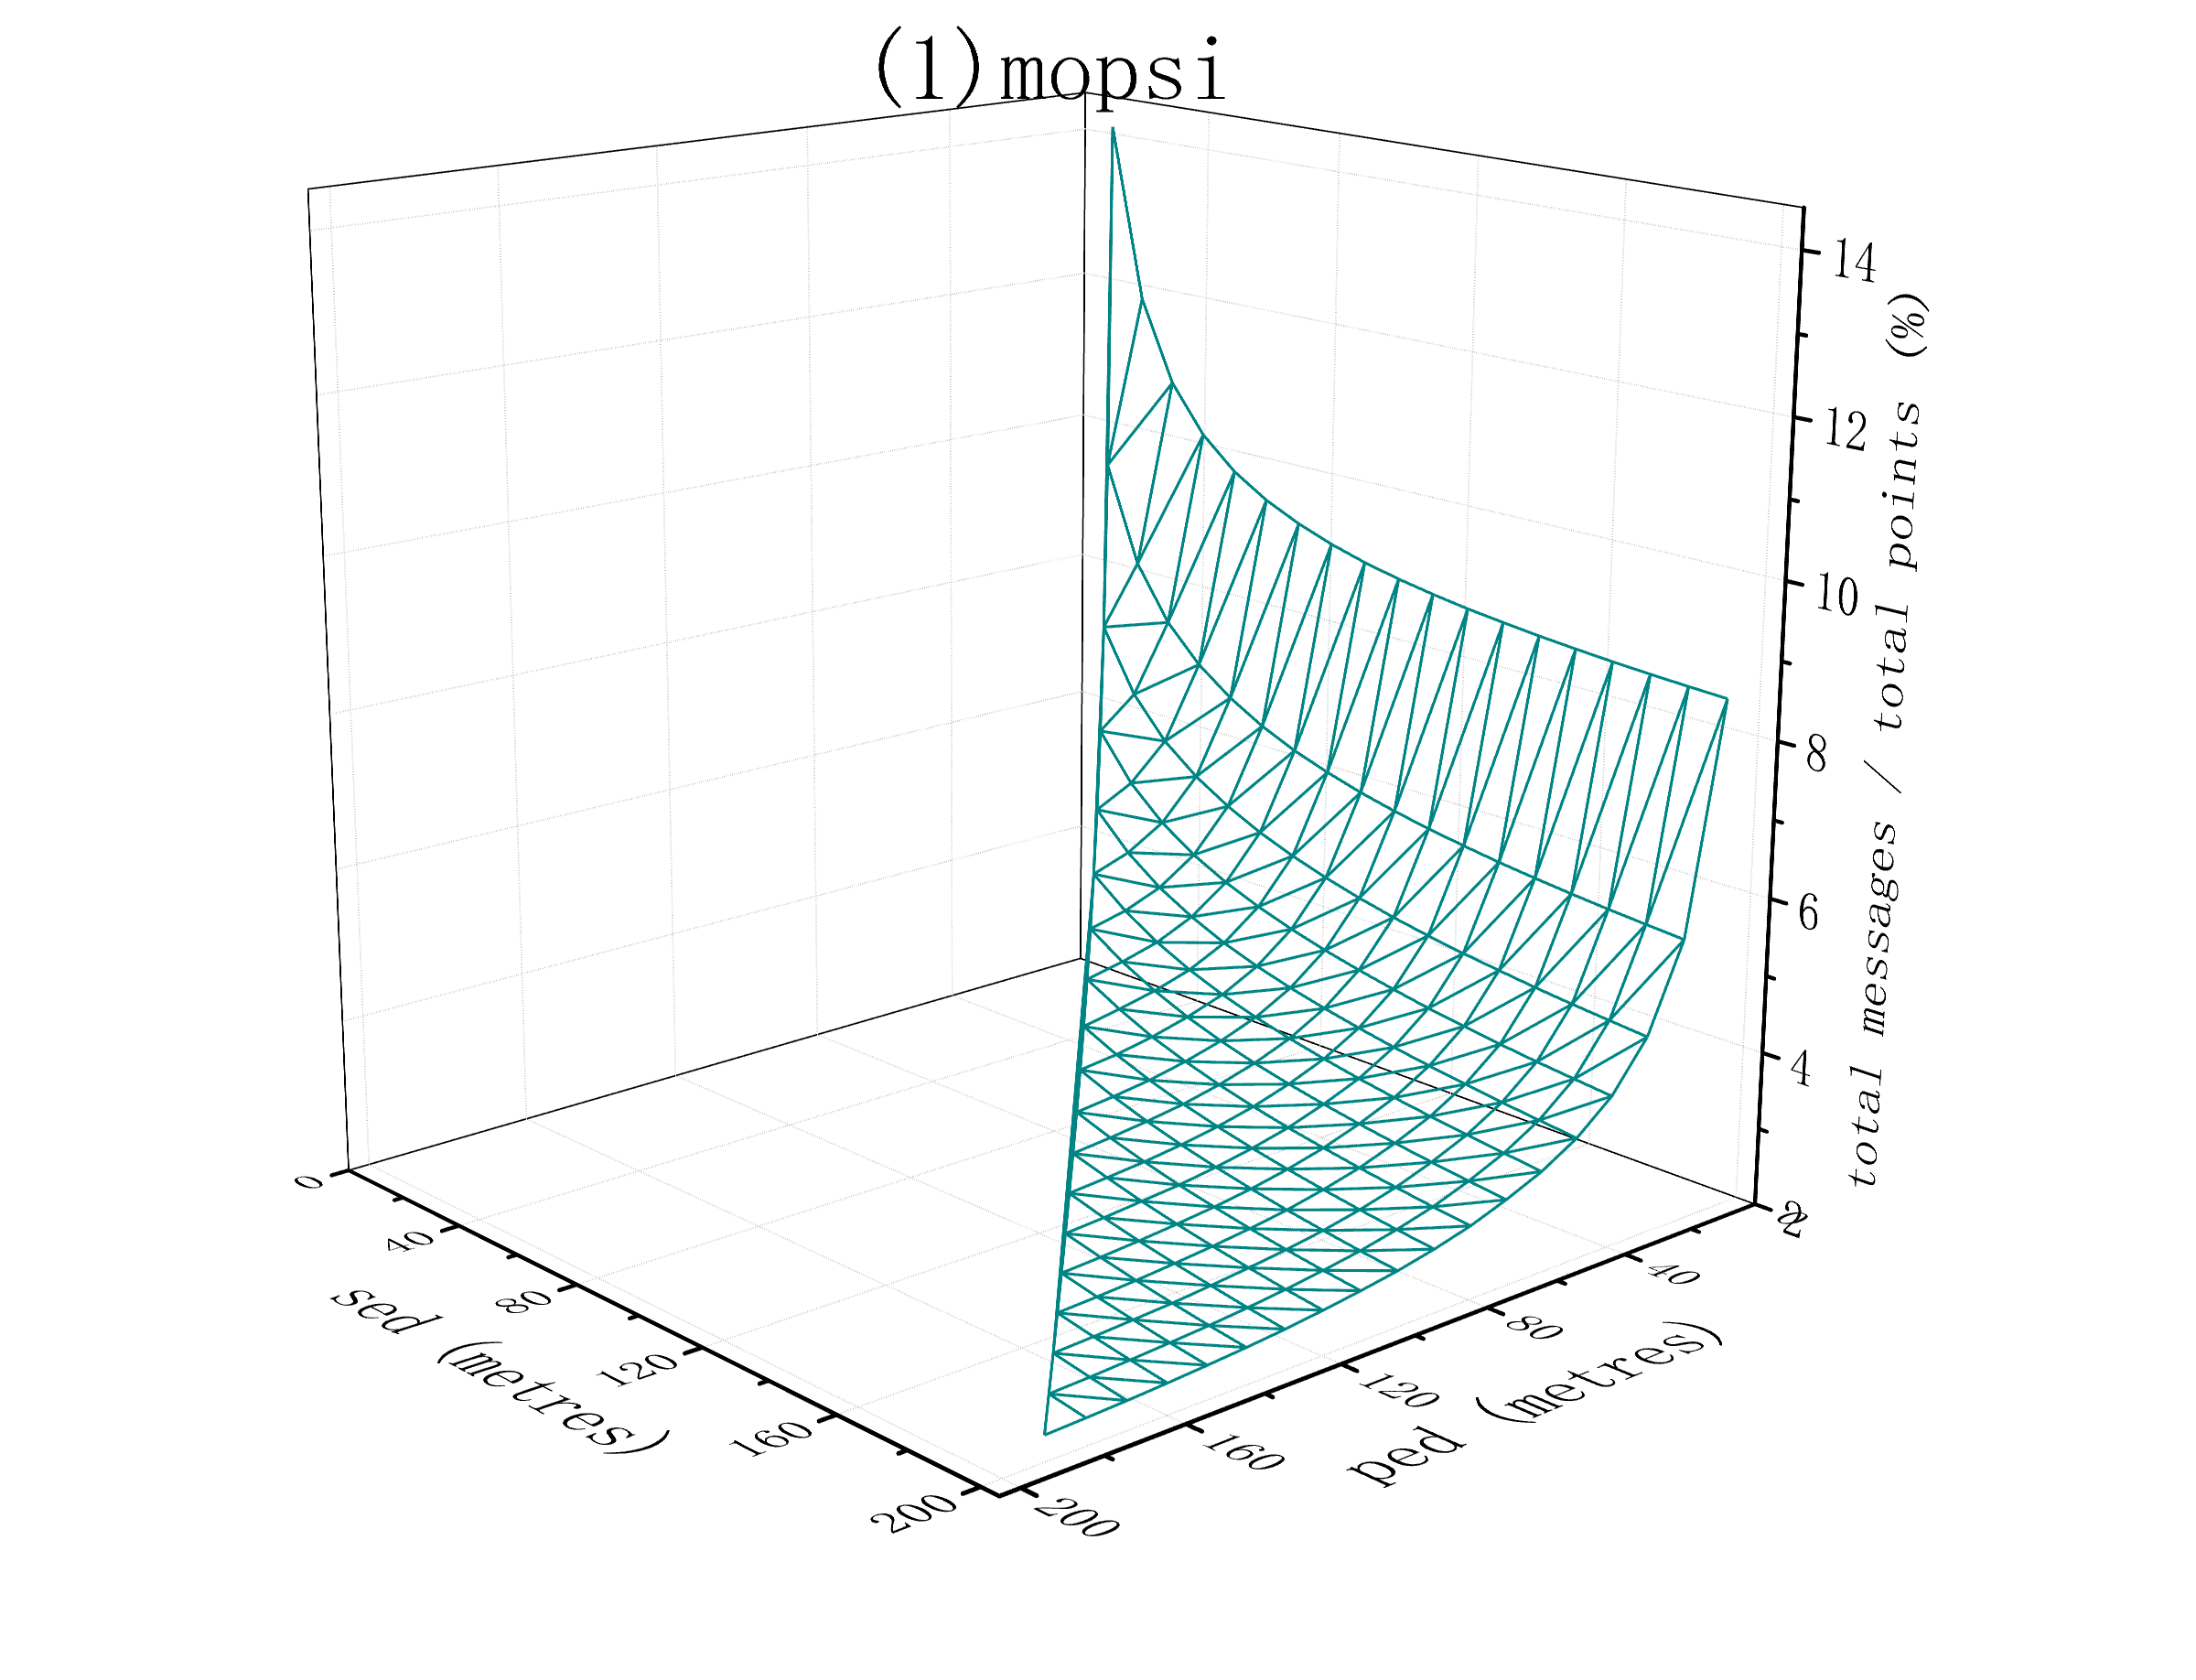
\includegraphics[scale = 0.210]{figures/Fig-BITT-mopsi-total-messages.png}\hspace{1ex}
	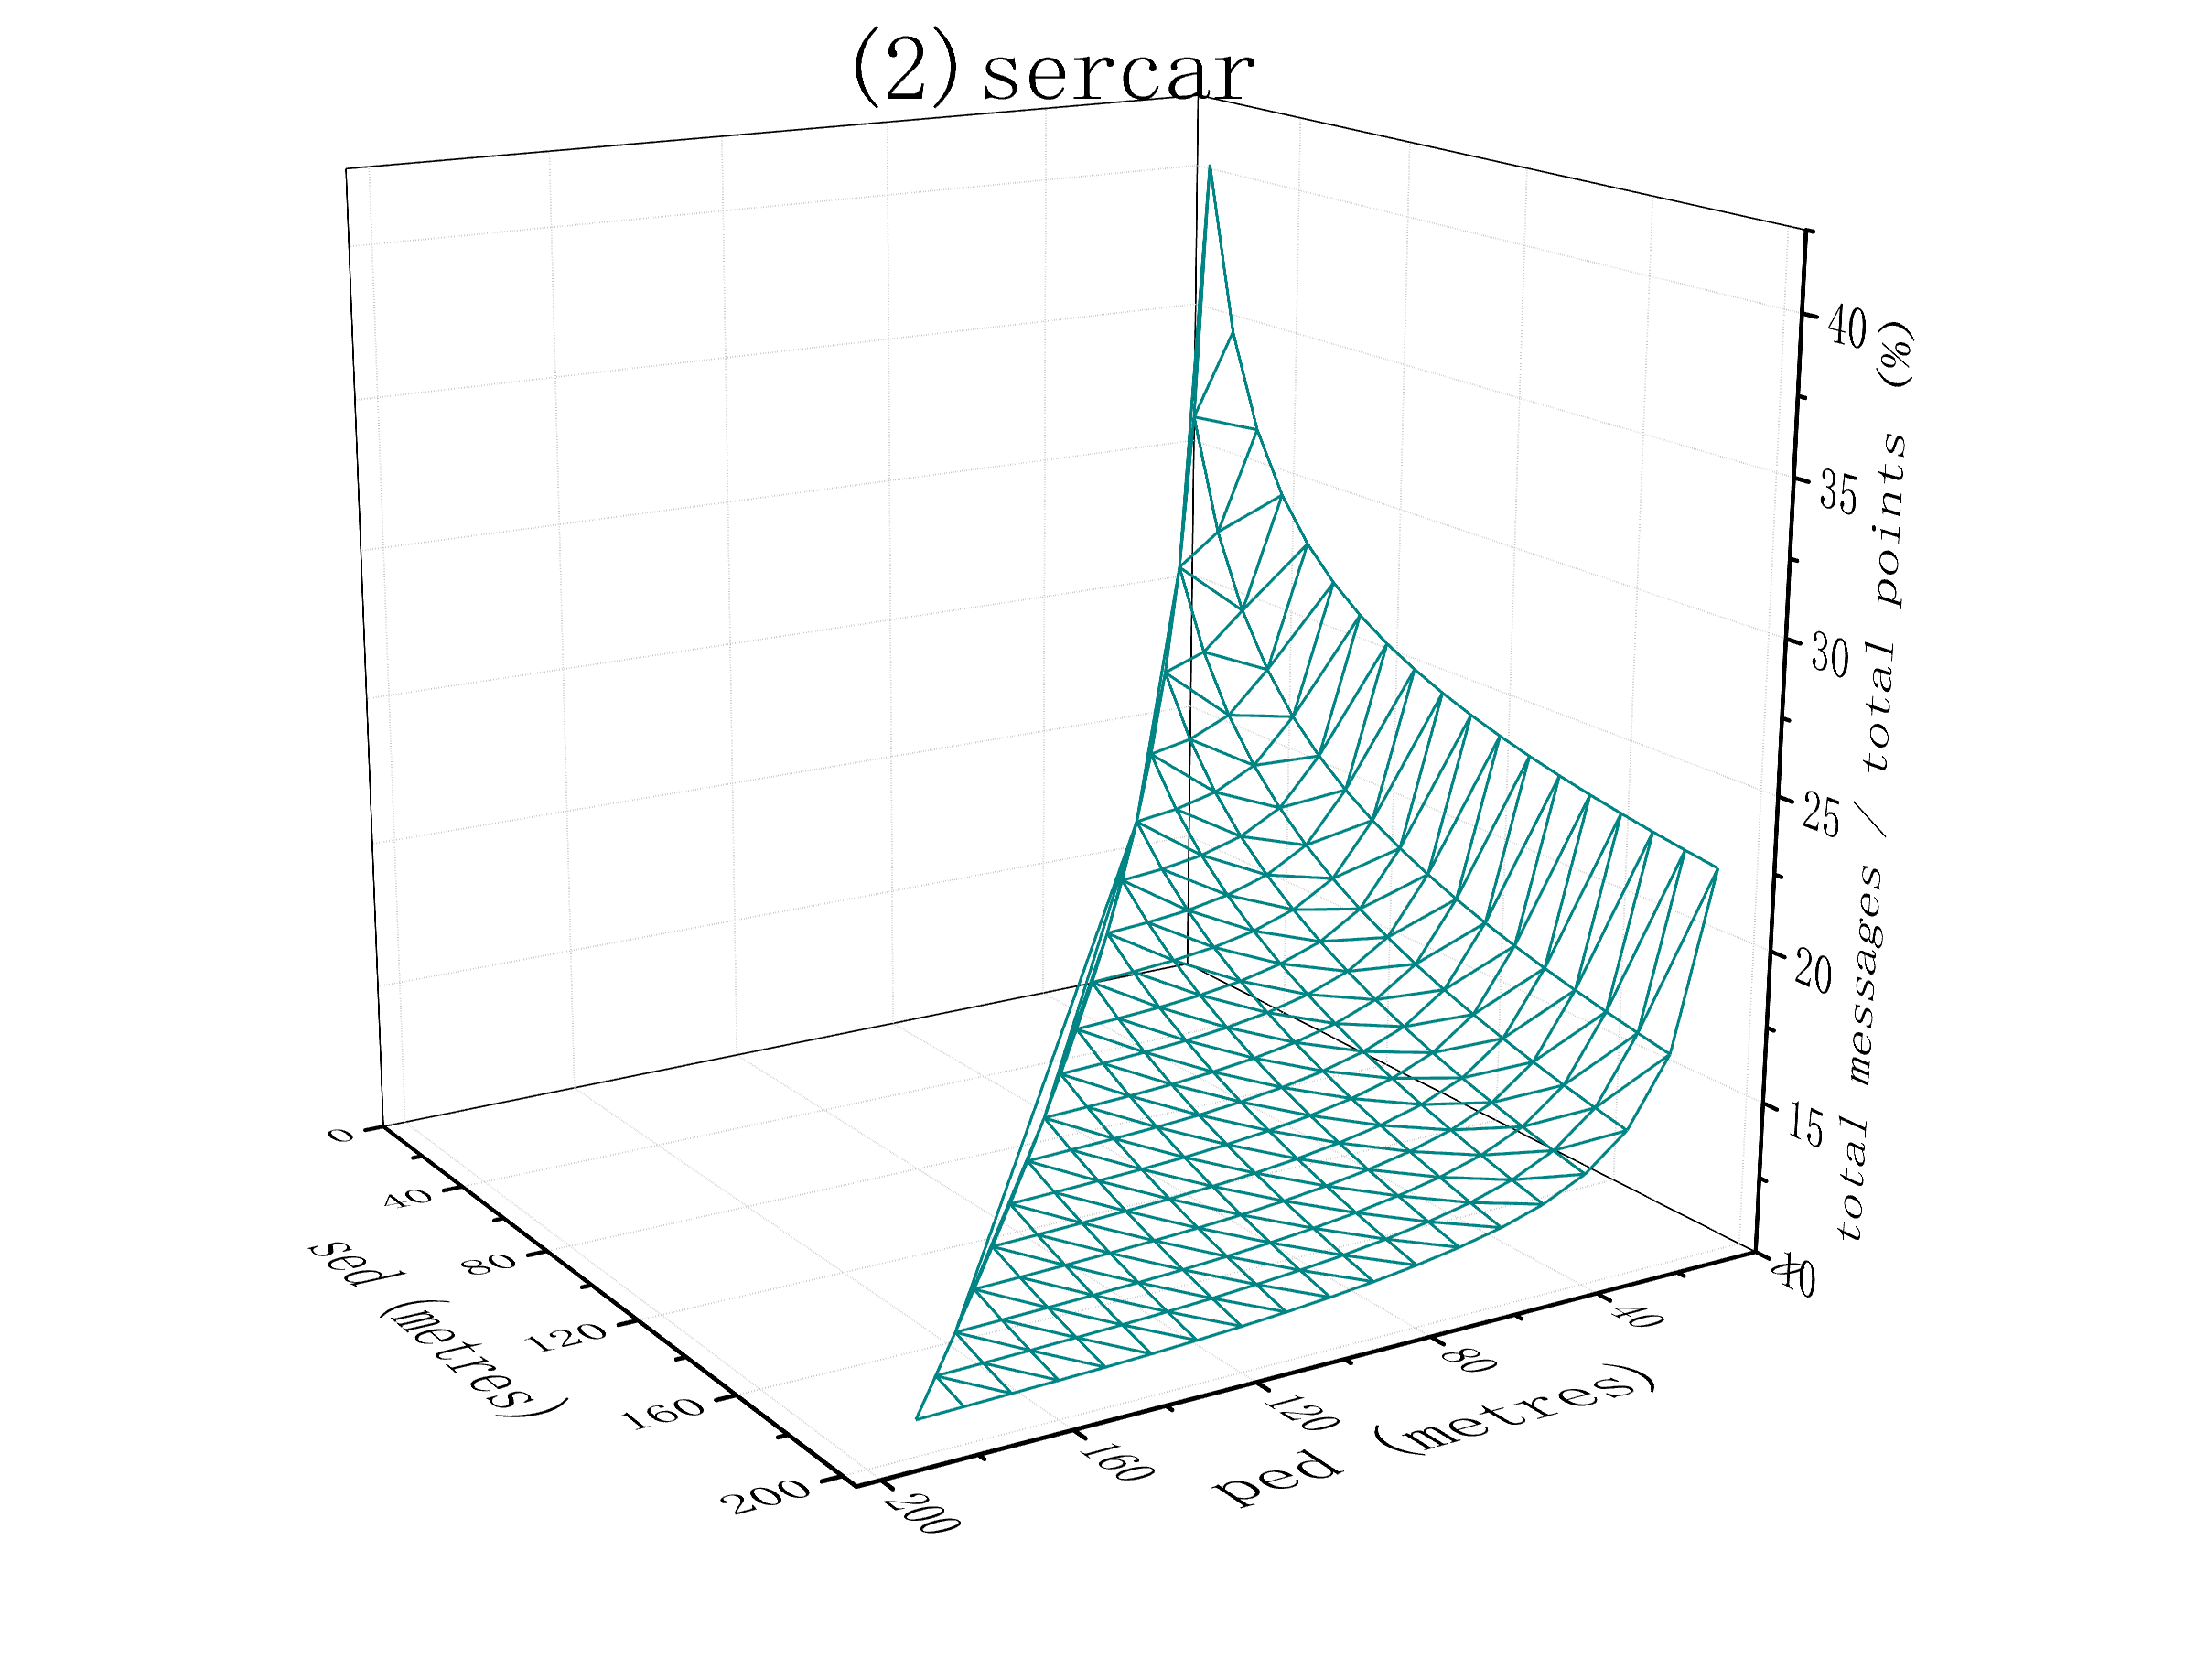
\includegraphics[scale = 0.210]{figures/Fig-BITT-sercar-total-messages.png}\hspace{1ex}
	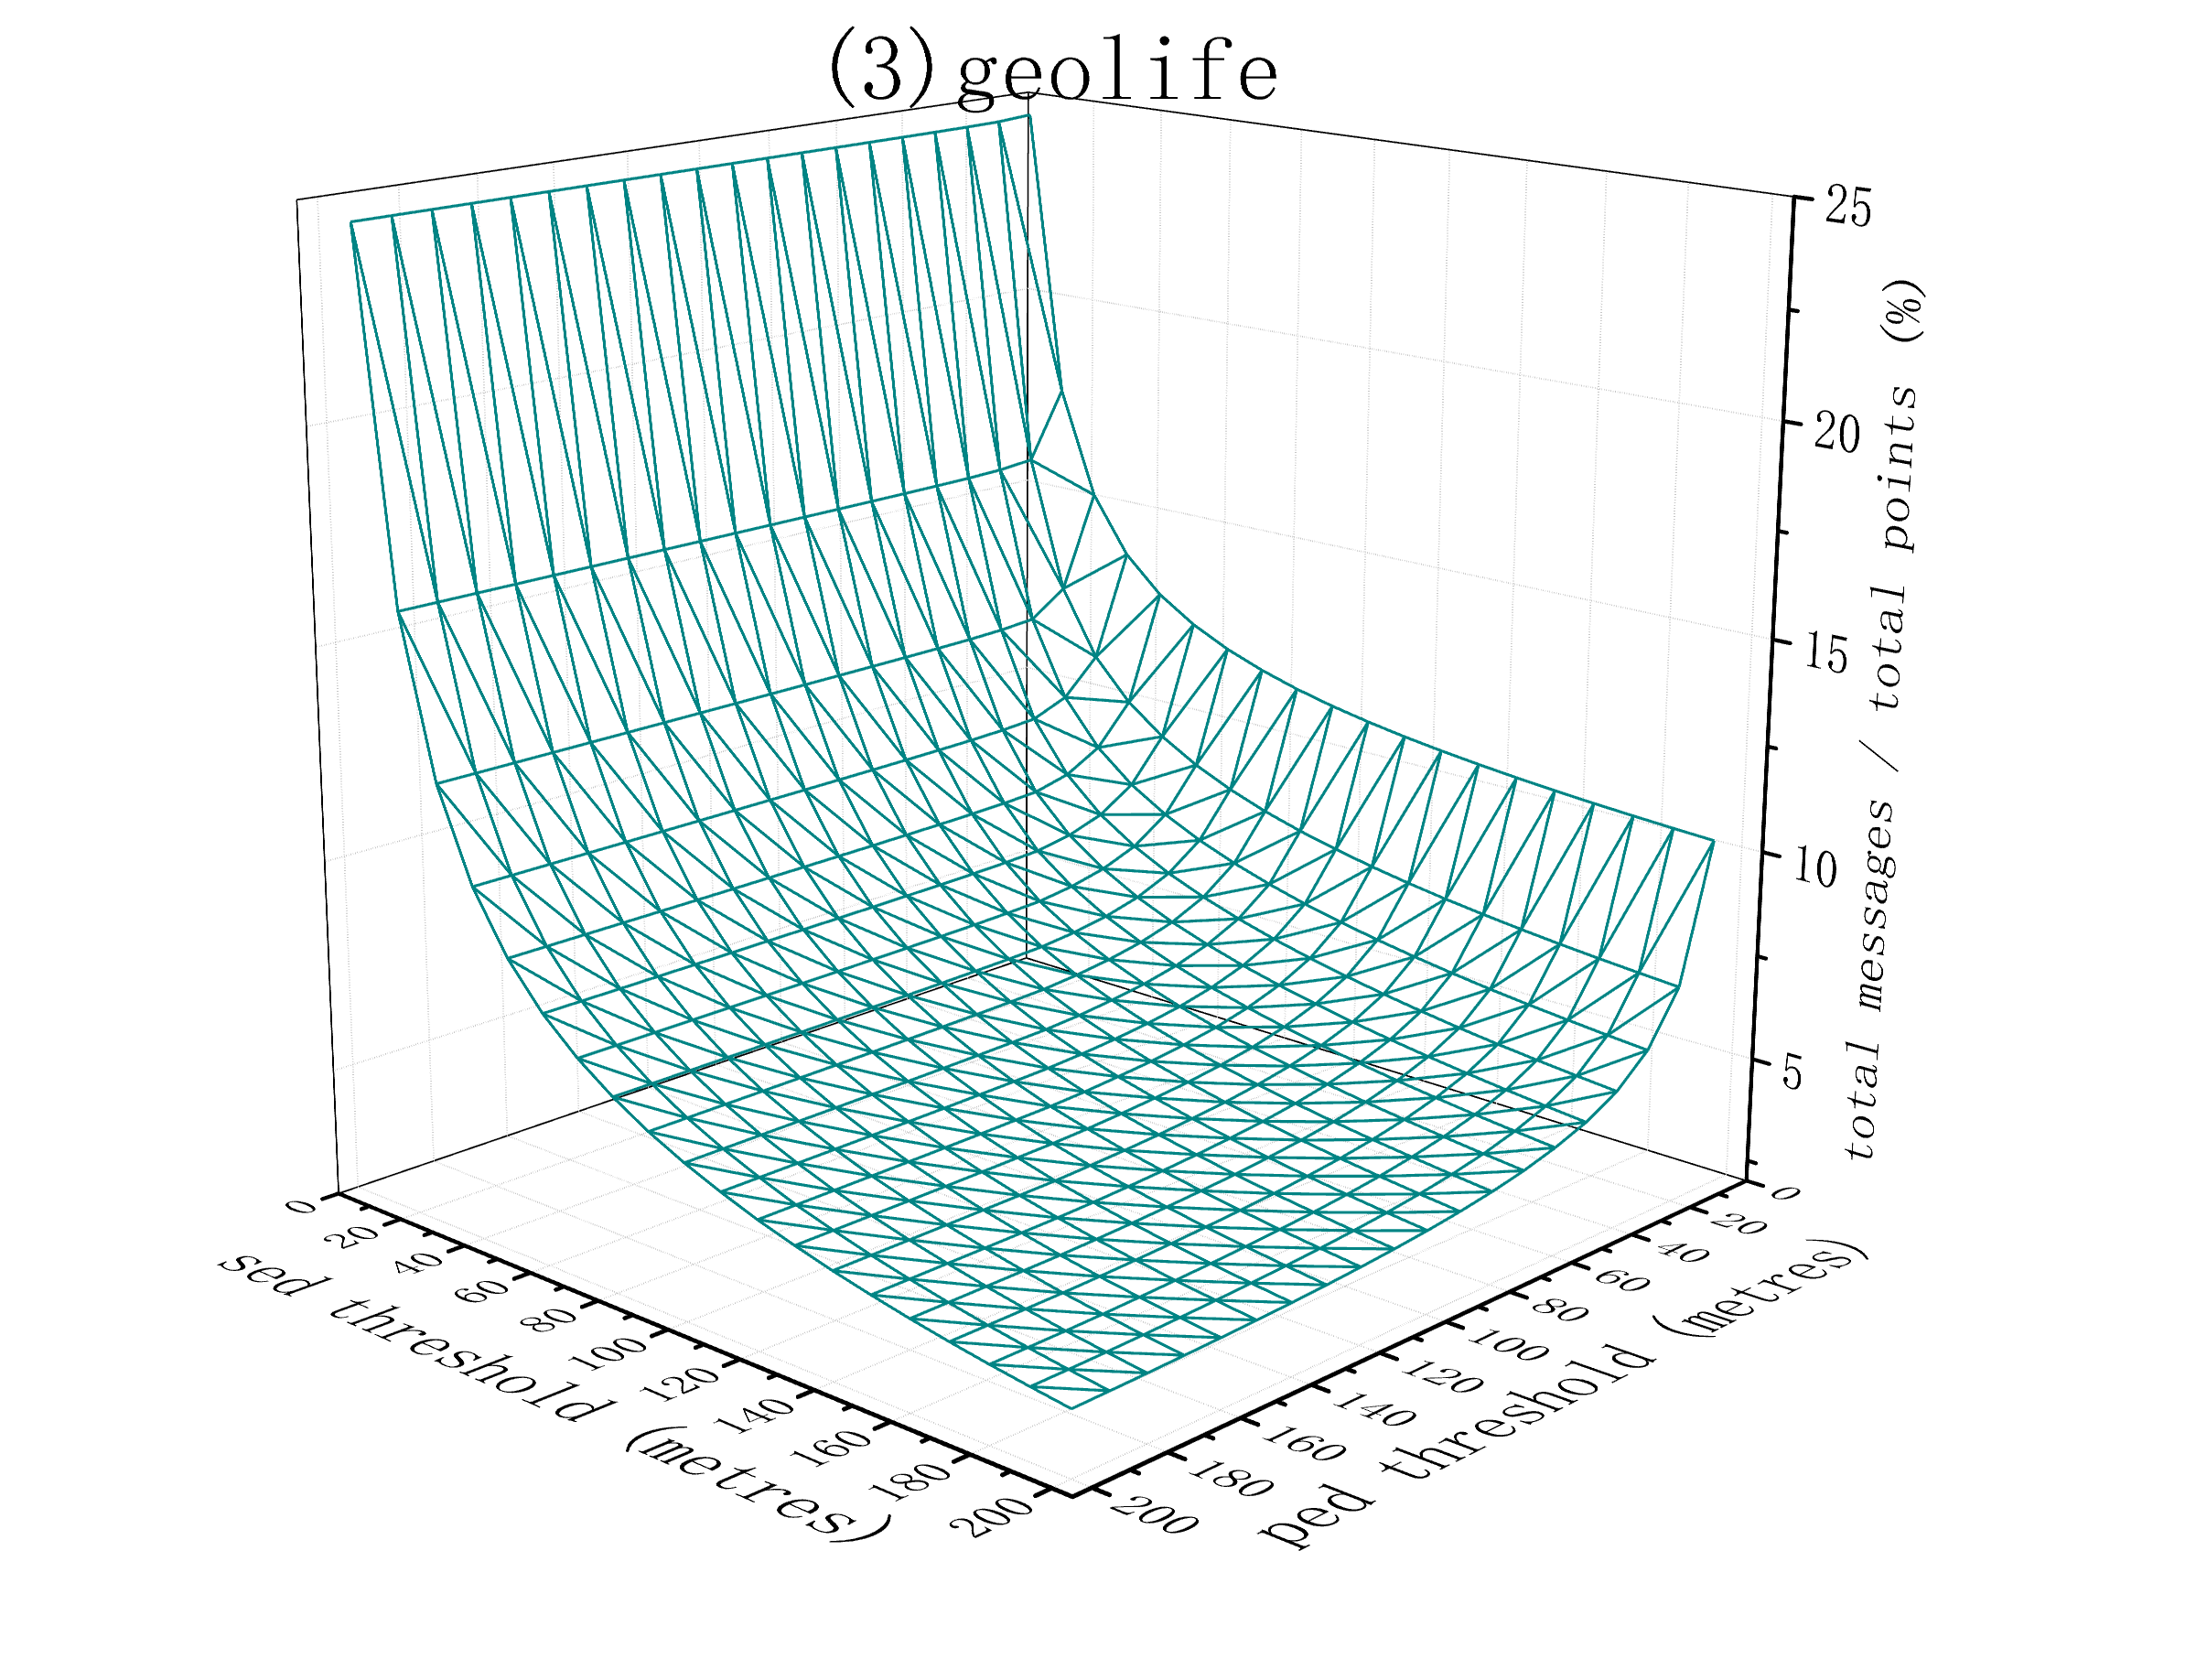
\includegraphics[scale = 0.210]{figures/Fig-BITT-geolife-total-messages.png}\hspace{1ex}
	%\vspace{-1ex}
	\caption{\small Evaluation of BITT total messages: varying error bounds $\epsilon_{sed}$ and $\epsilon_{ped}$.}
	\label{fig:bitt-total-message}
	%\vspace{-1ex}
\end{figure*}




\begin{figure*}[tb!]
	\centering
	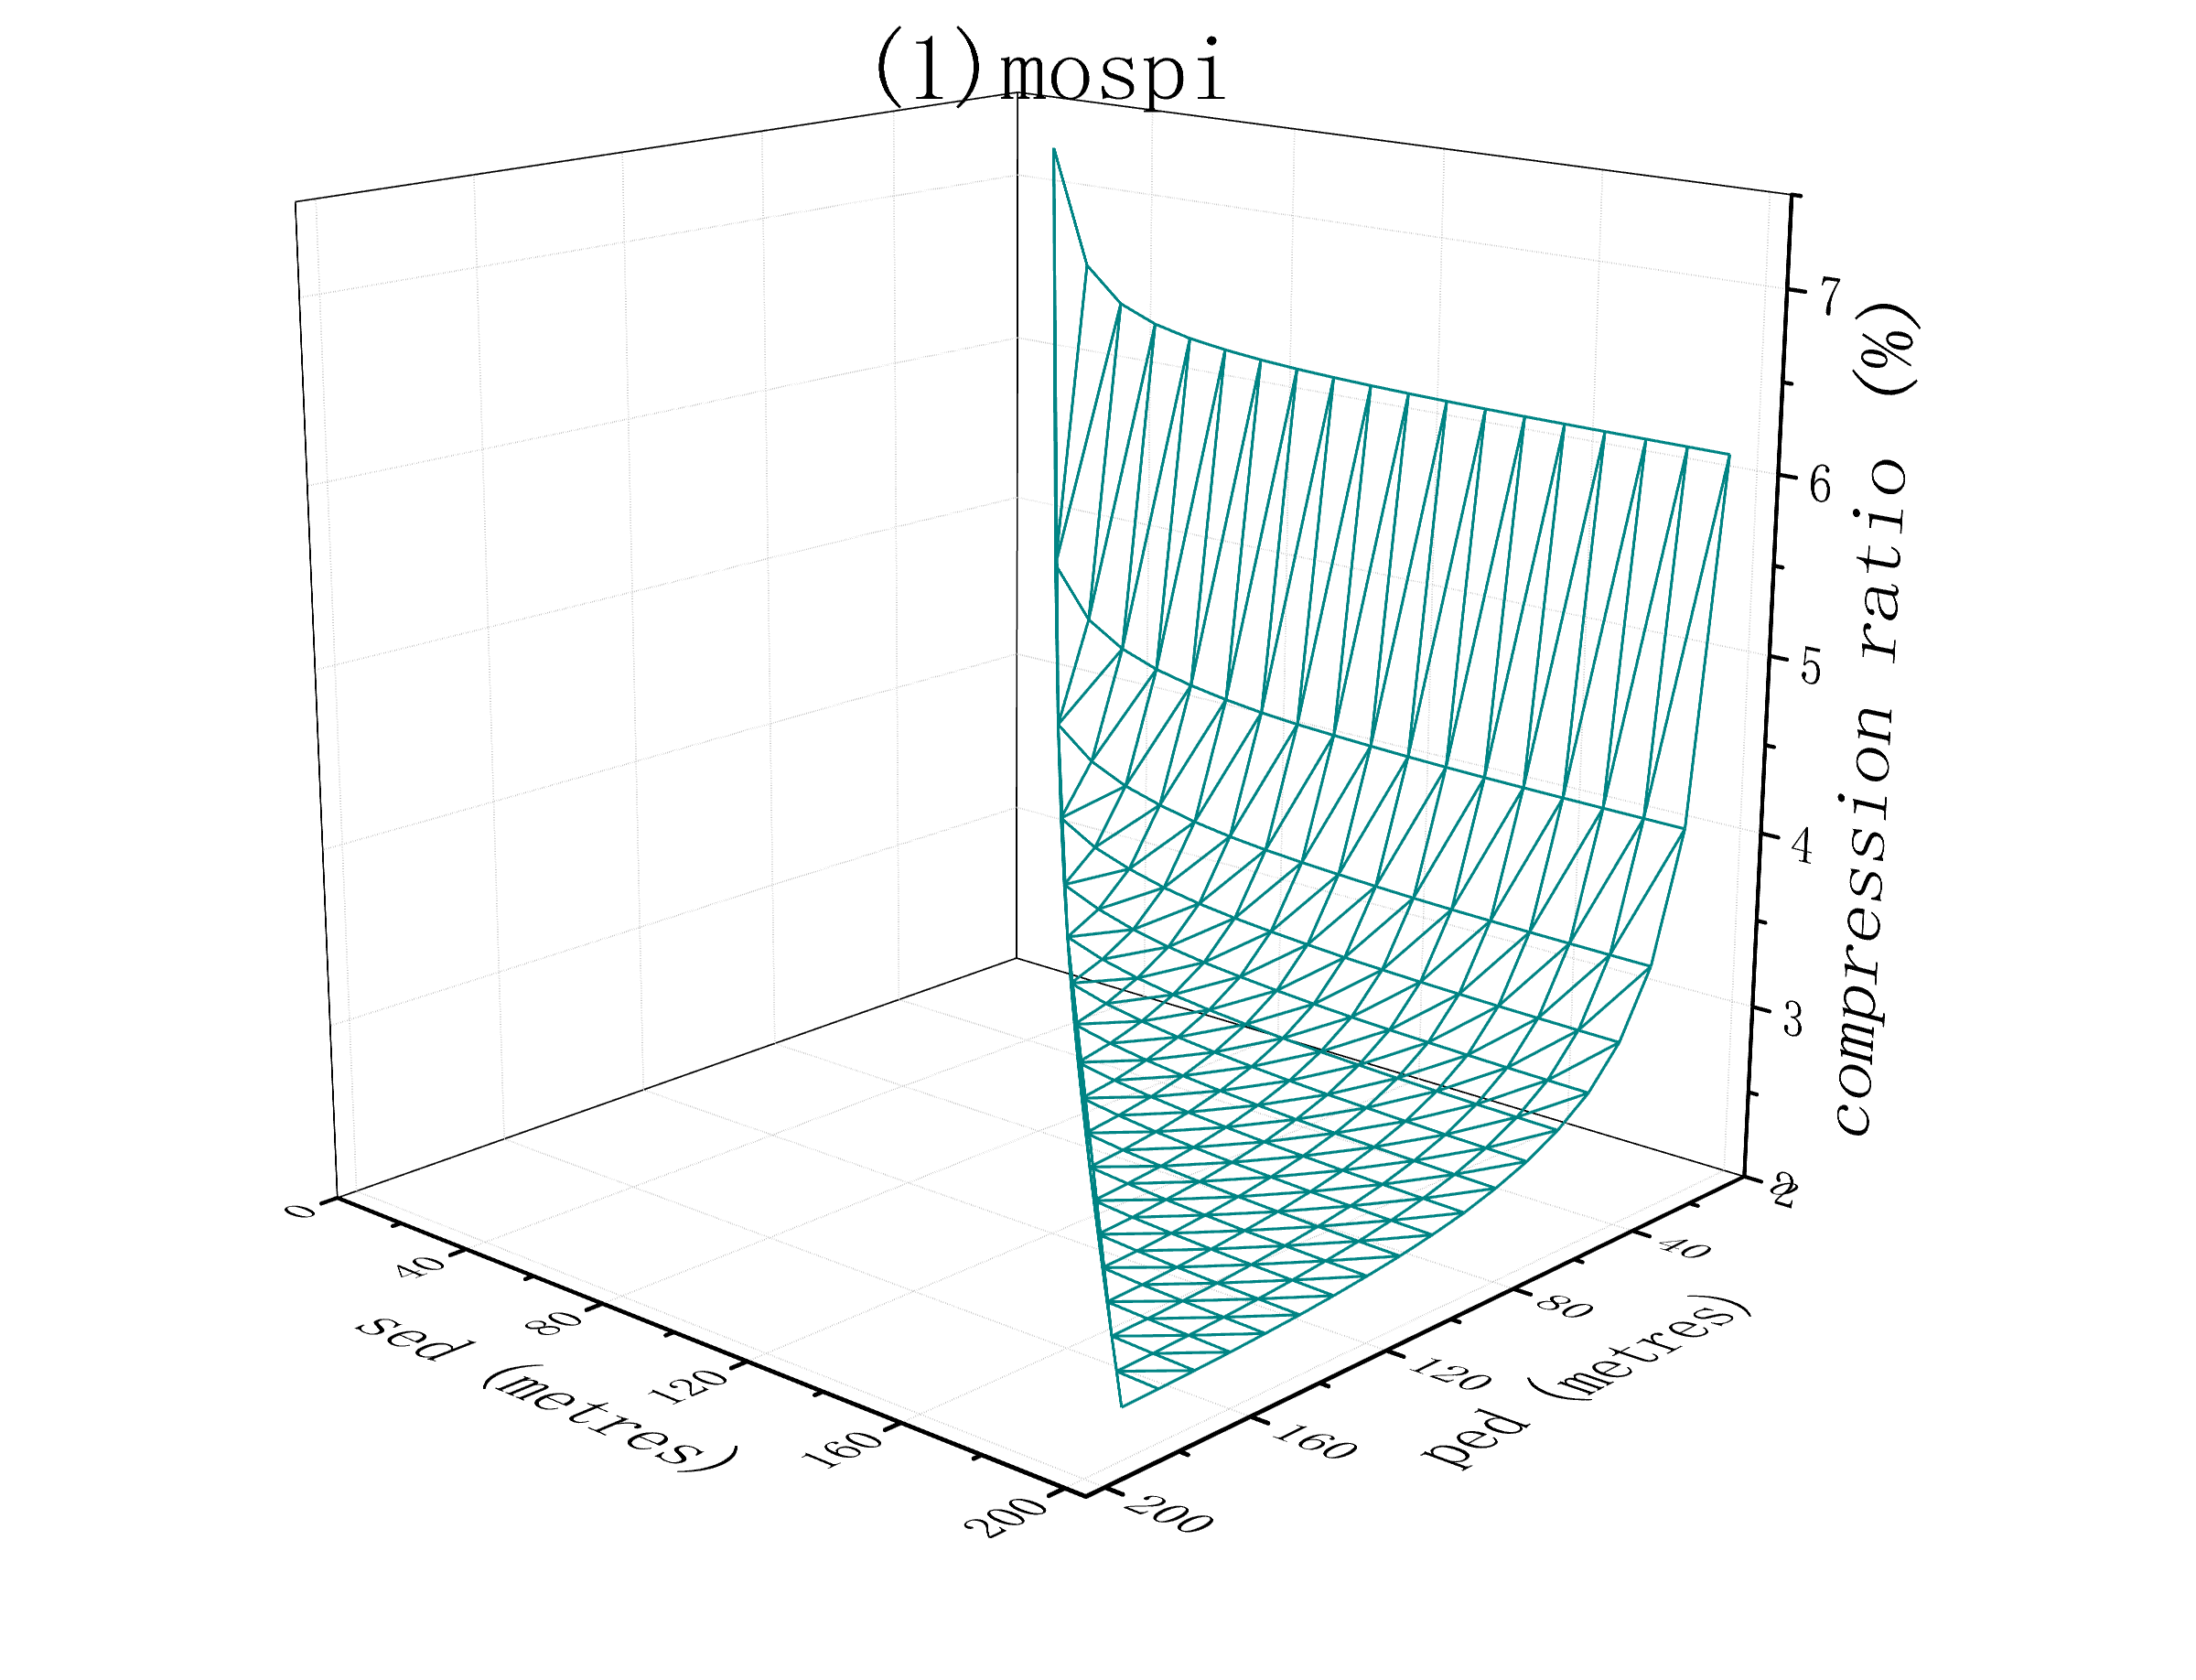
\includegraphics[scale = 0.210]{figures/Fig-BITT-mopsi-compression-ratio.png}\hspace{1ex}
	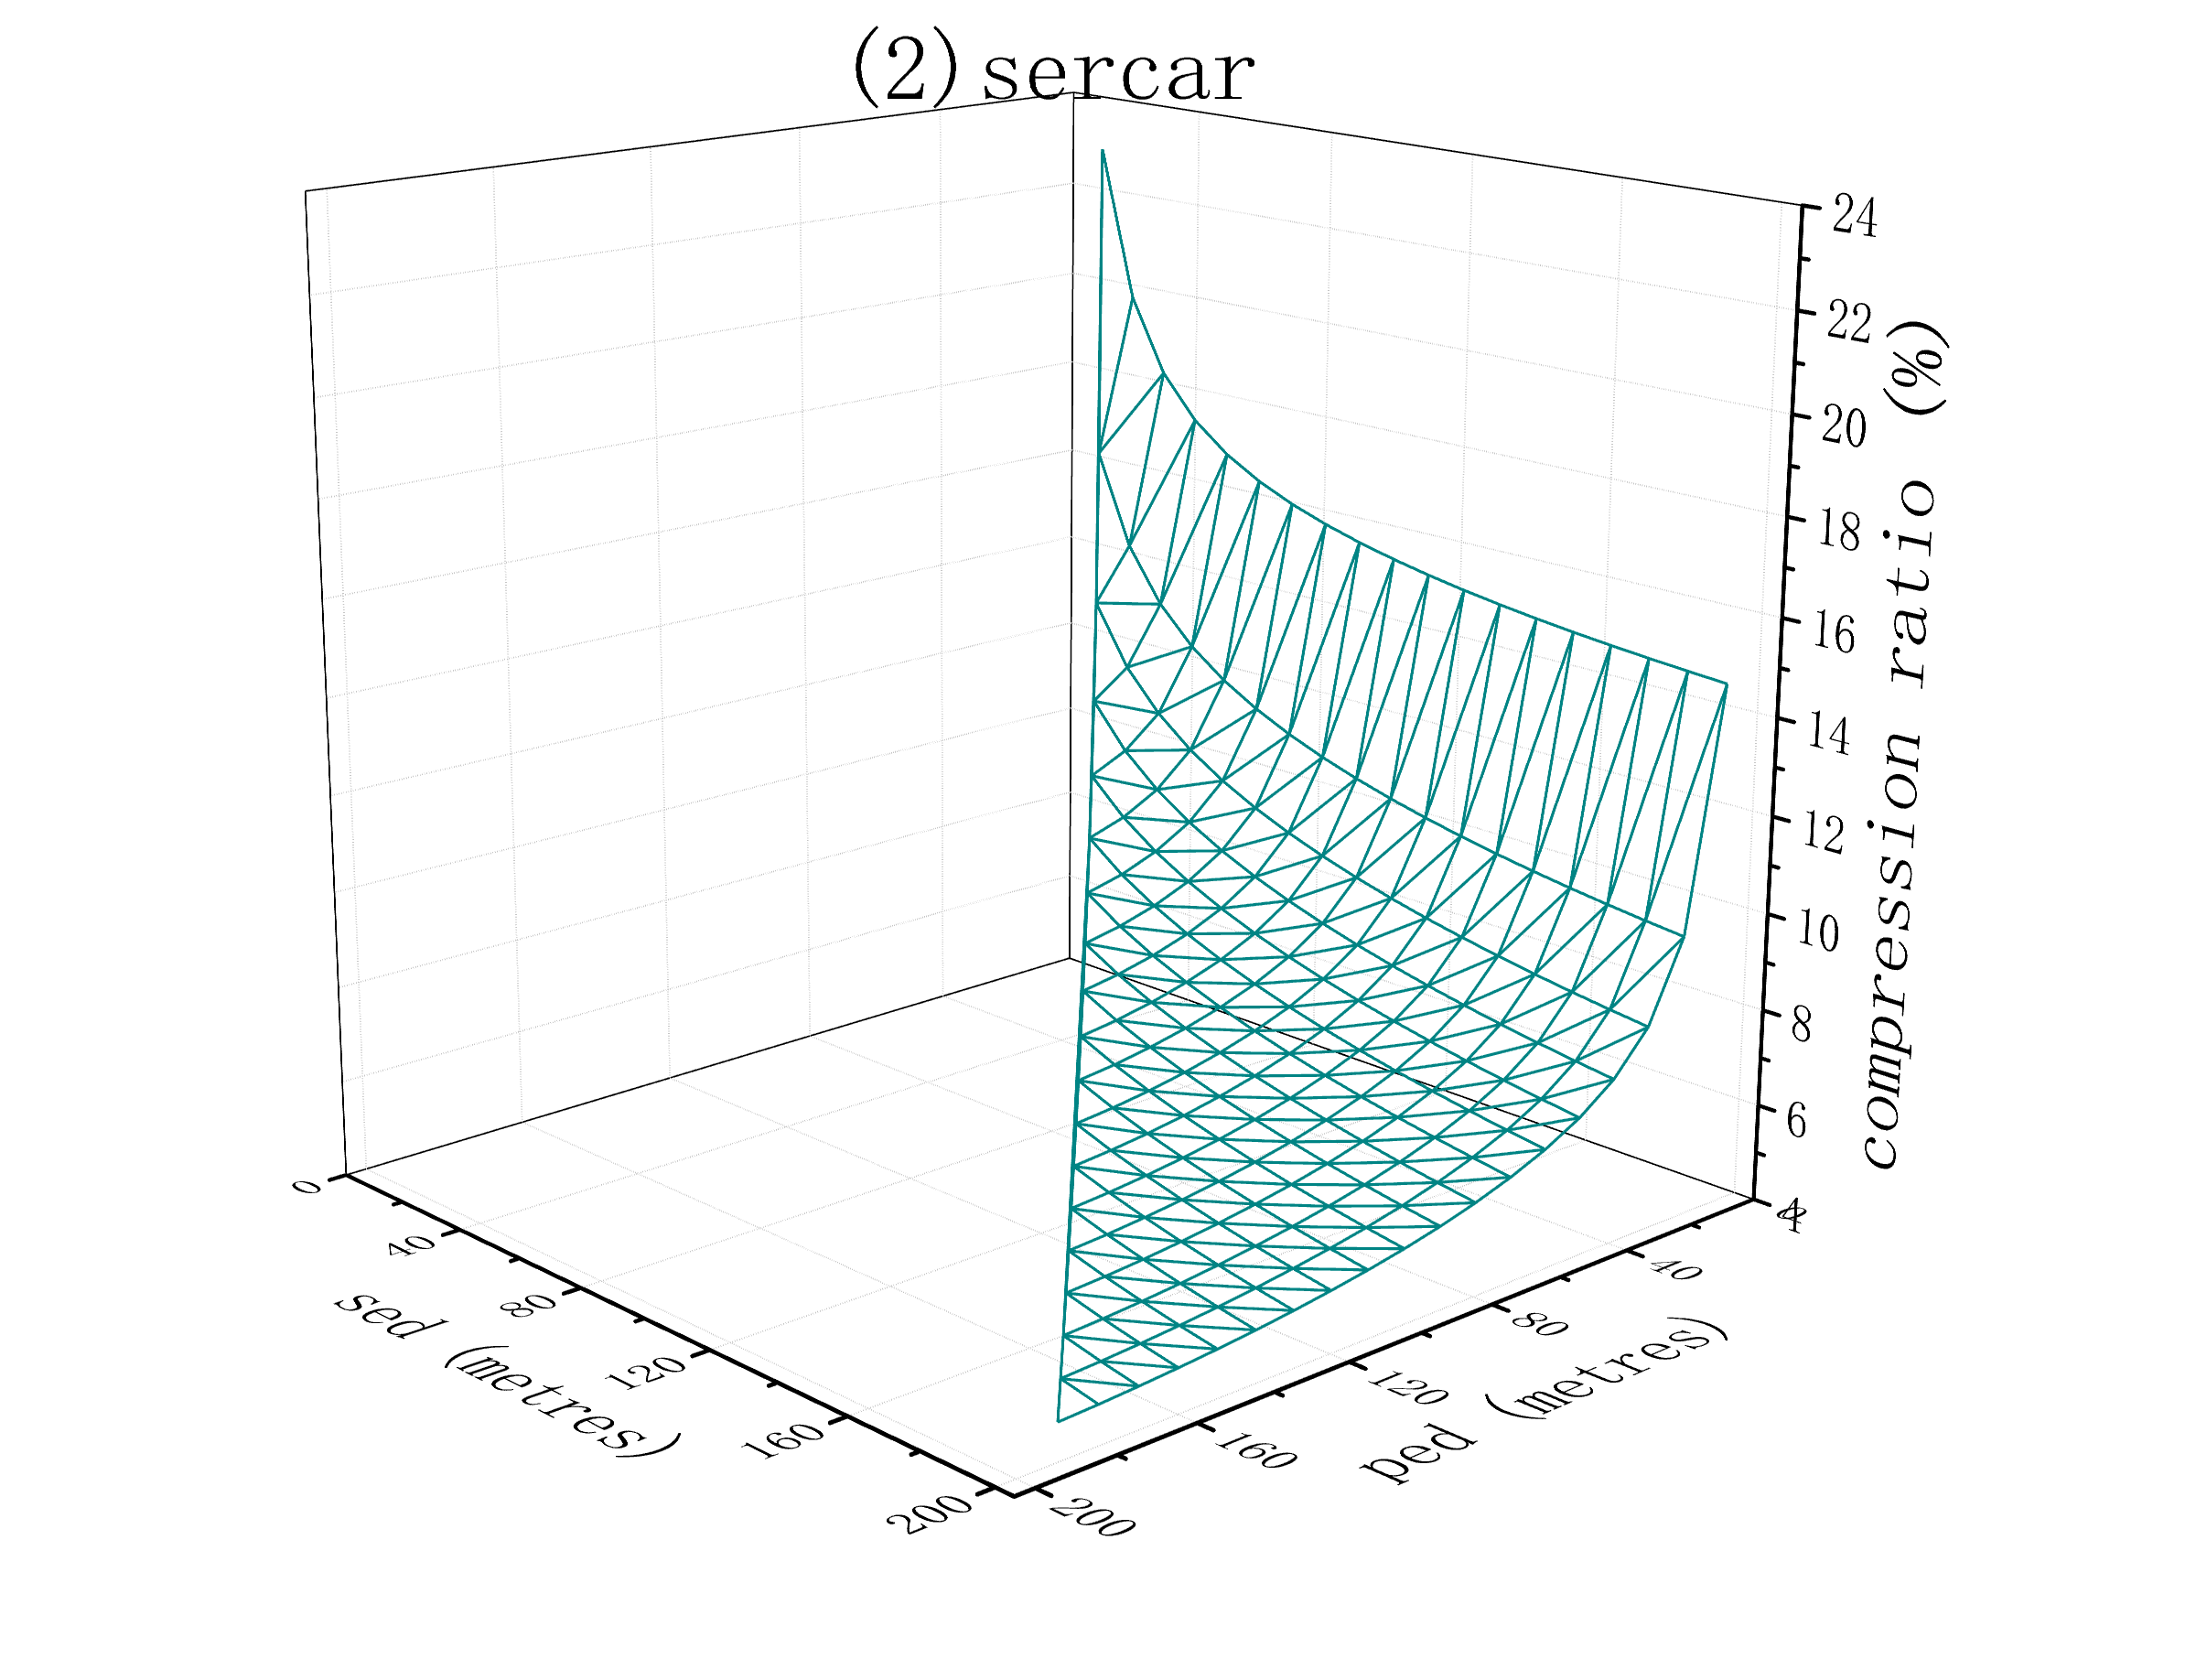
\includegraphics[scale = 0.210]{figures/Fig-BITT-sercar-compression-ratio.png}\hspace{1ex}
	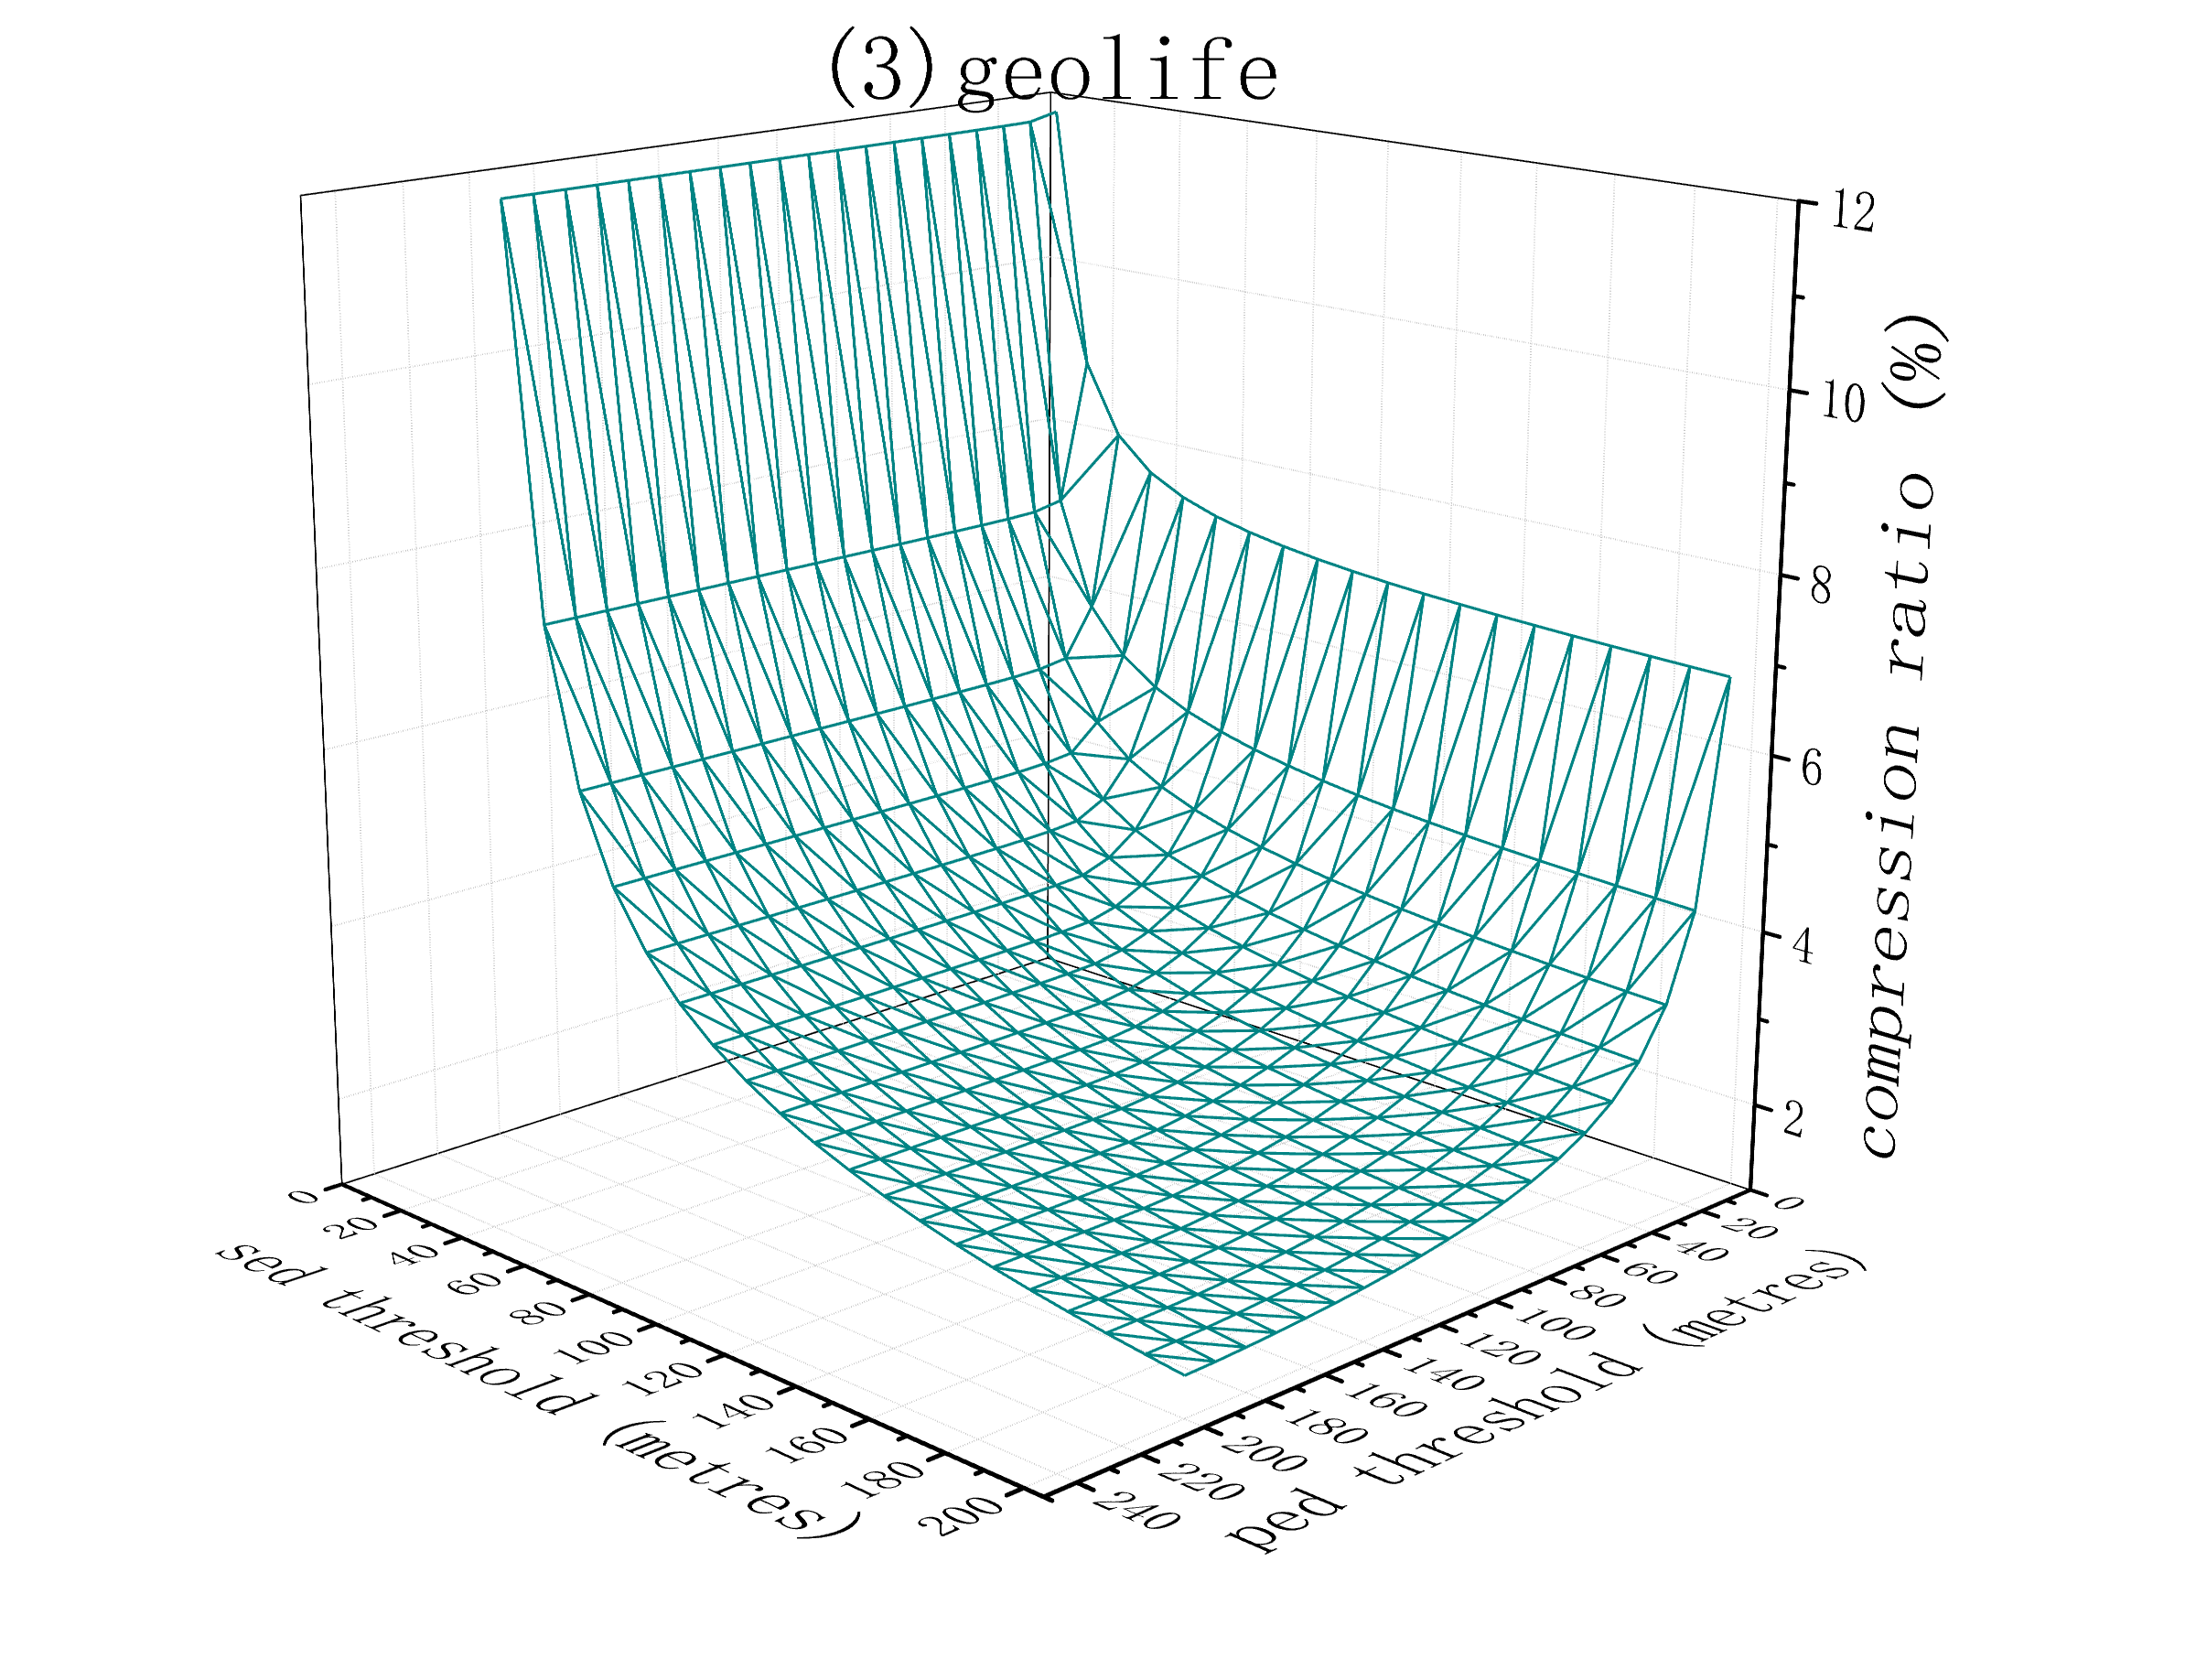
\includegraphics[scale = 0.210]{figures/Fig-BITT-geolife-compression-ratio.png}\hspace{1ex}
	%\vspace{-1ex}
	\caption{\small Evaluation of BITT compression ratio: varying error bounds $\epsilon_{sed}$ and $\epsilon_{ped}$.}
	\label{fig:bitt-compression-ratio}
	%\vspace{-1ex}
\end{figure*}


\begin{figure*}[tb!]
	\centering
	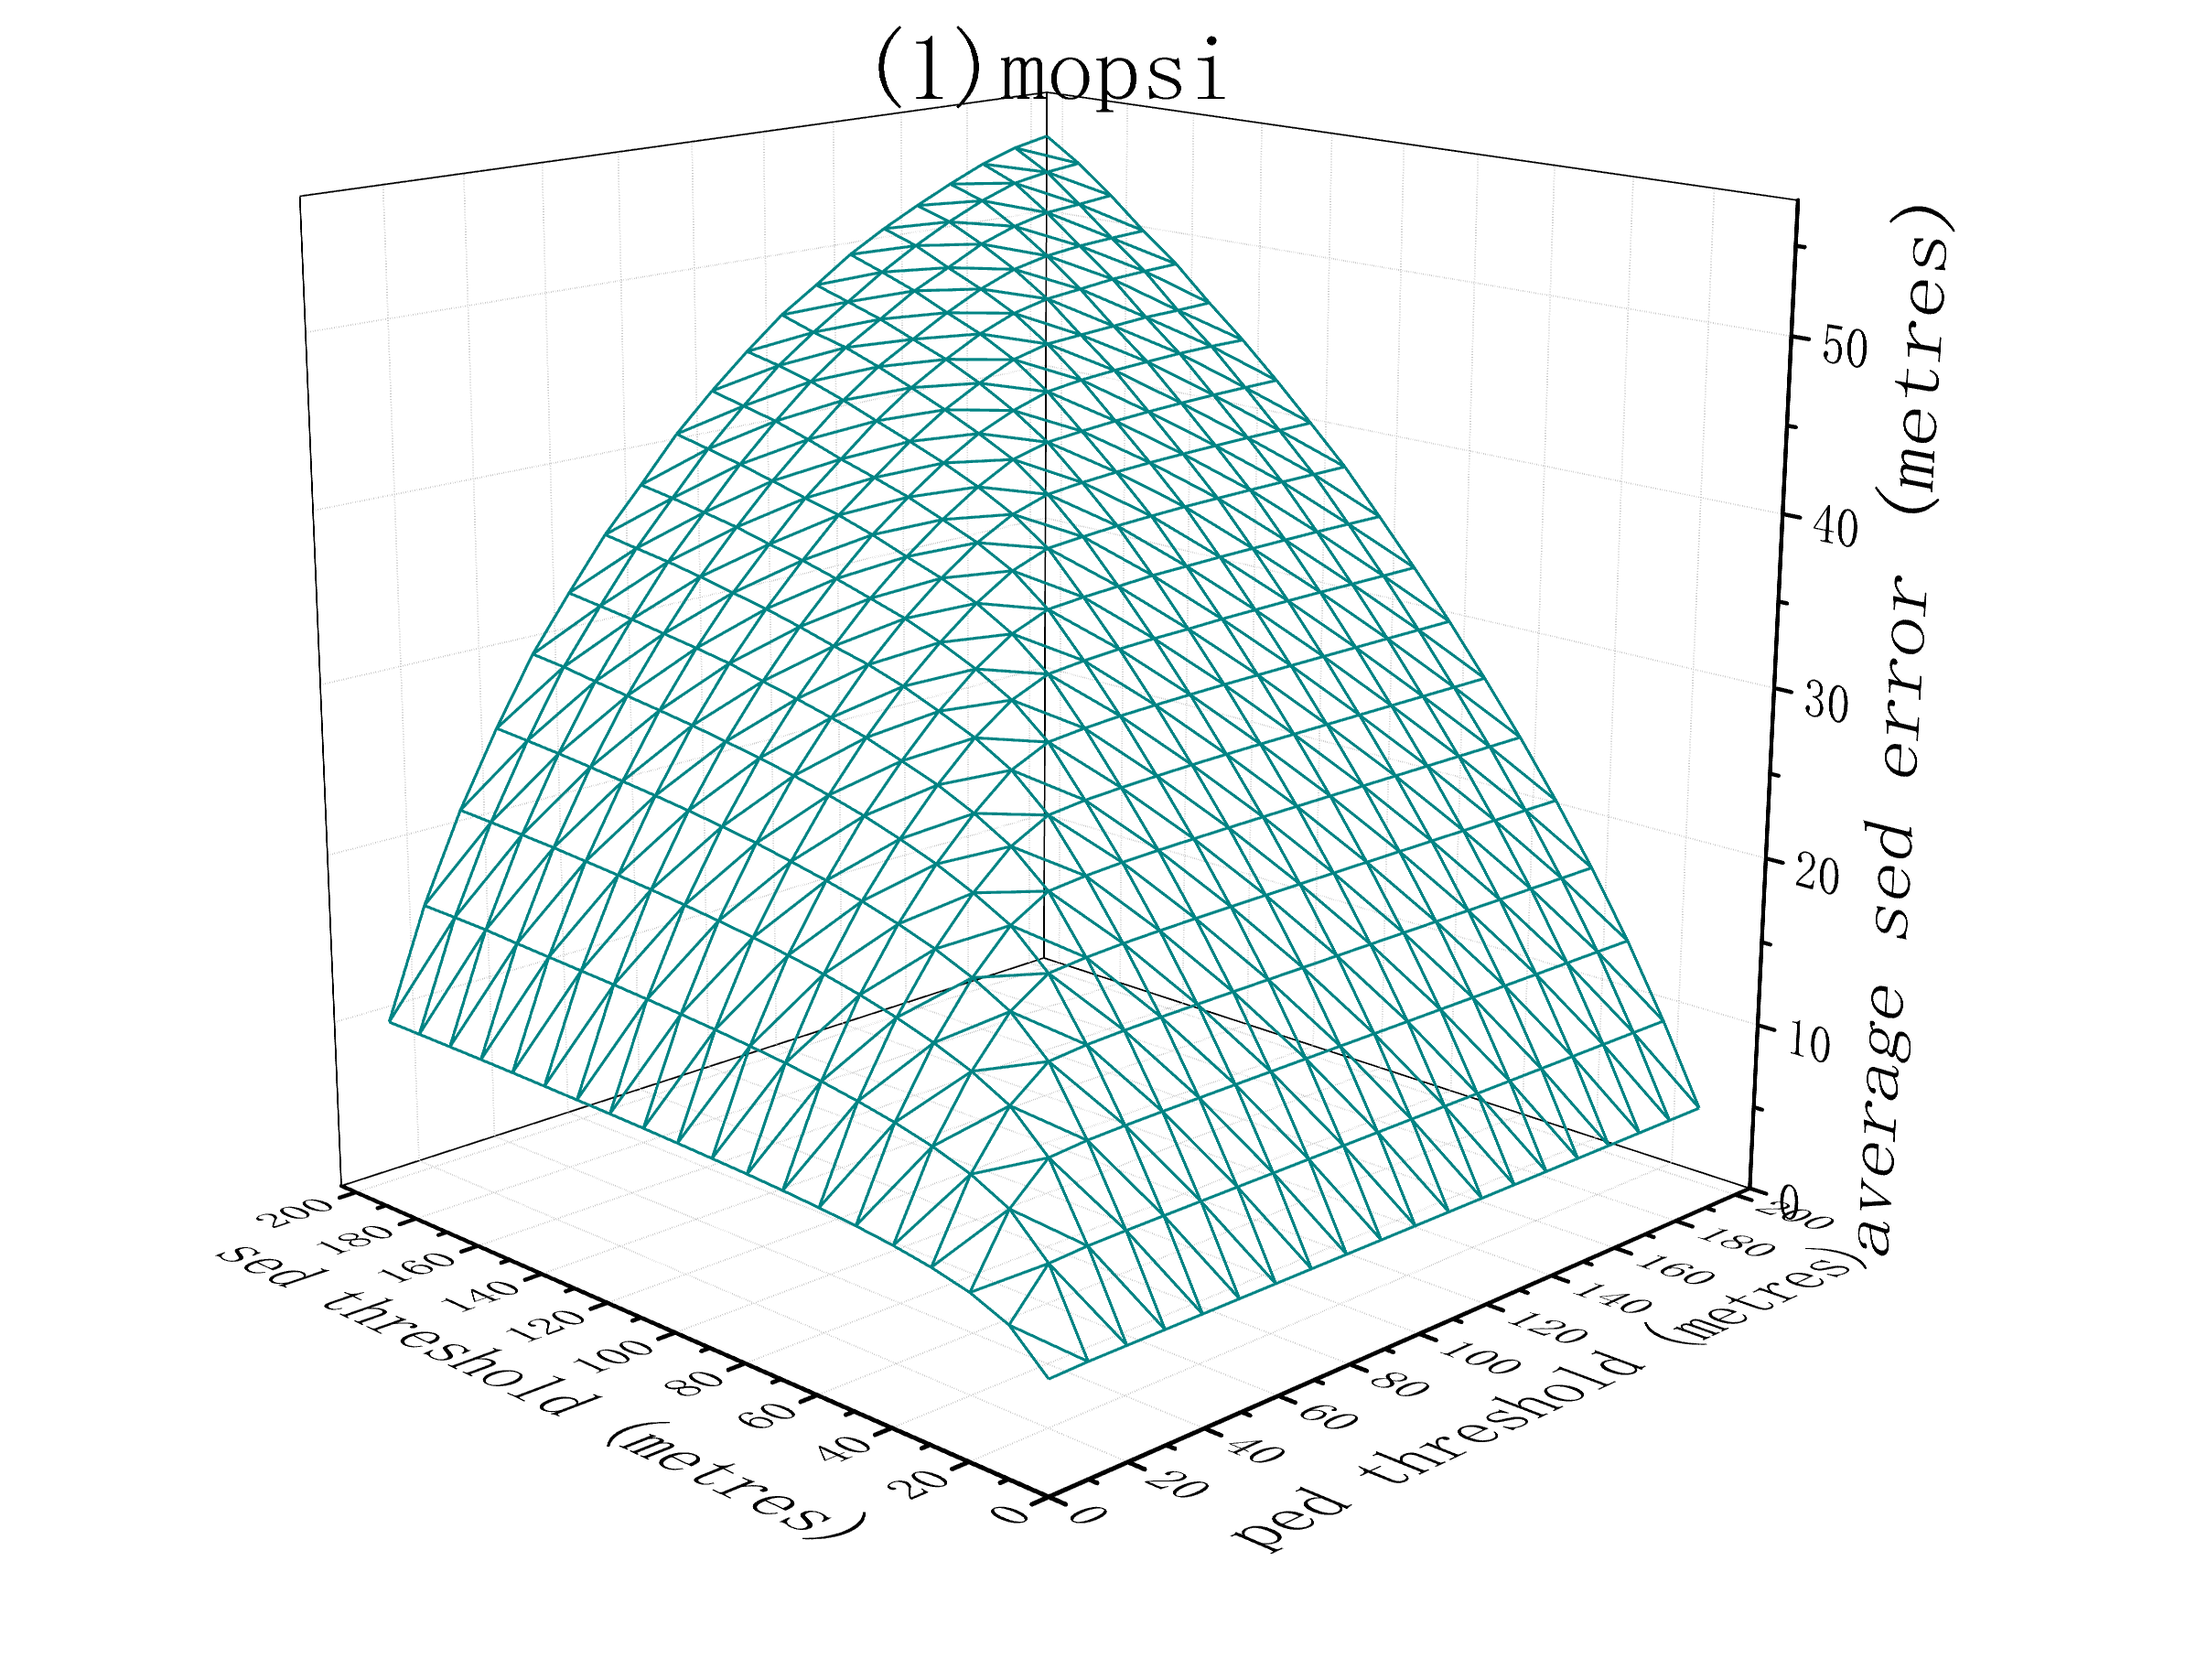
\includegraphics[scale = 0.210]{figures/Fig-BITT-mopsi-sed-error.png}\hspace{1ex}
	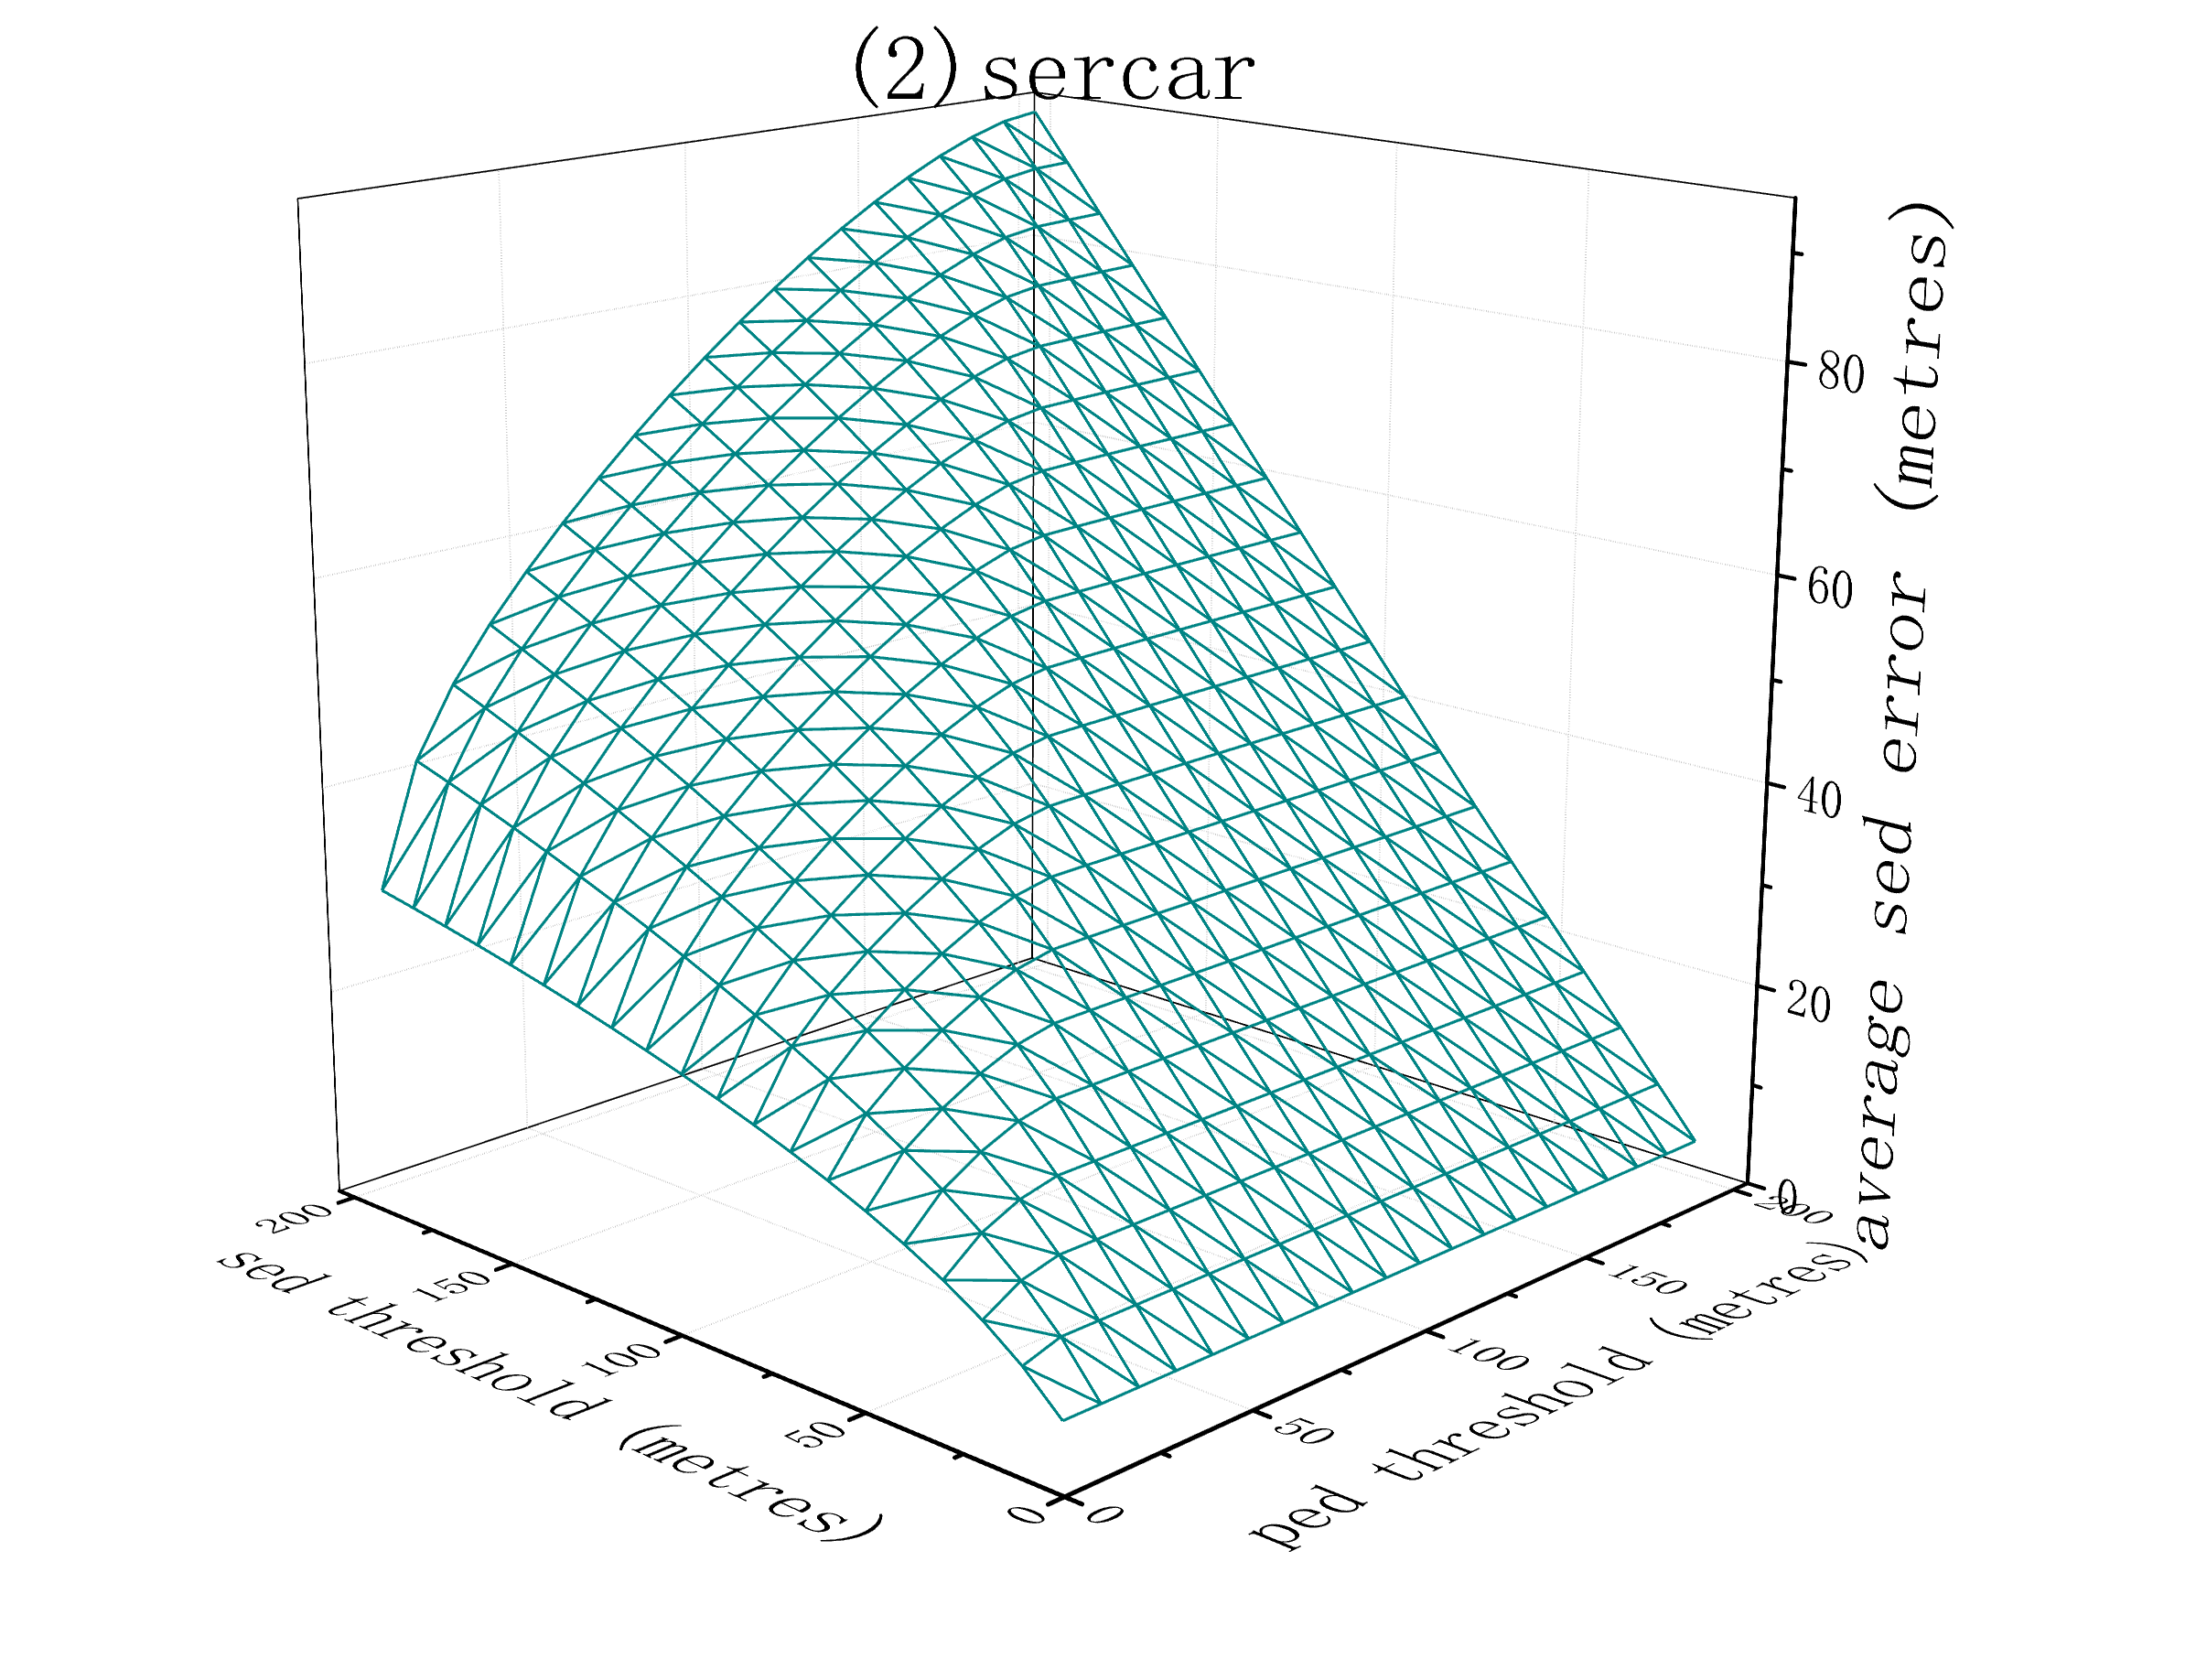
\includegraphics[scale = 0.210]{figures/Fig-BITT-sercar-sed-error.png}\hspace{1ex}
	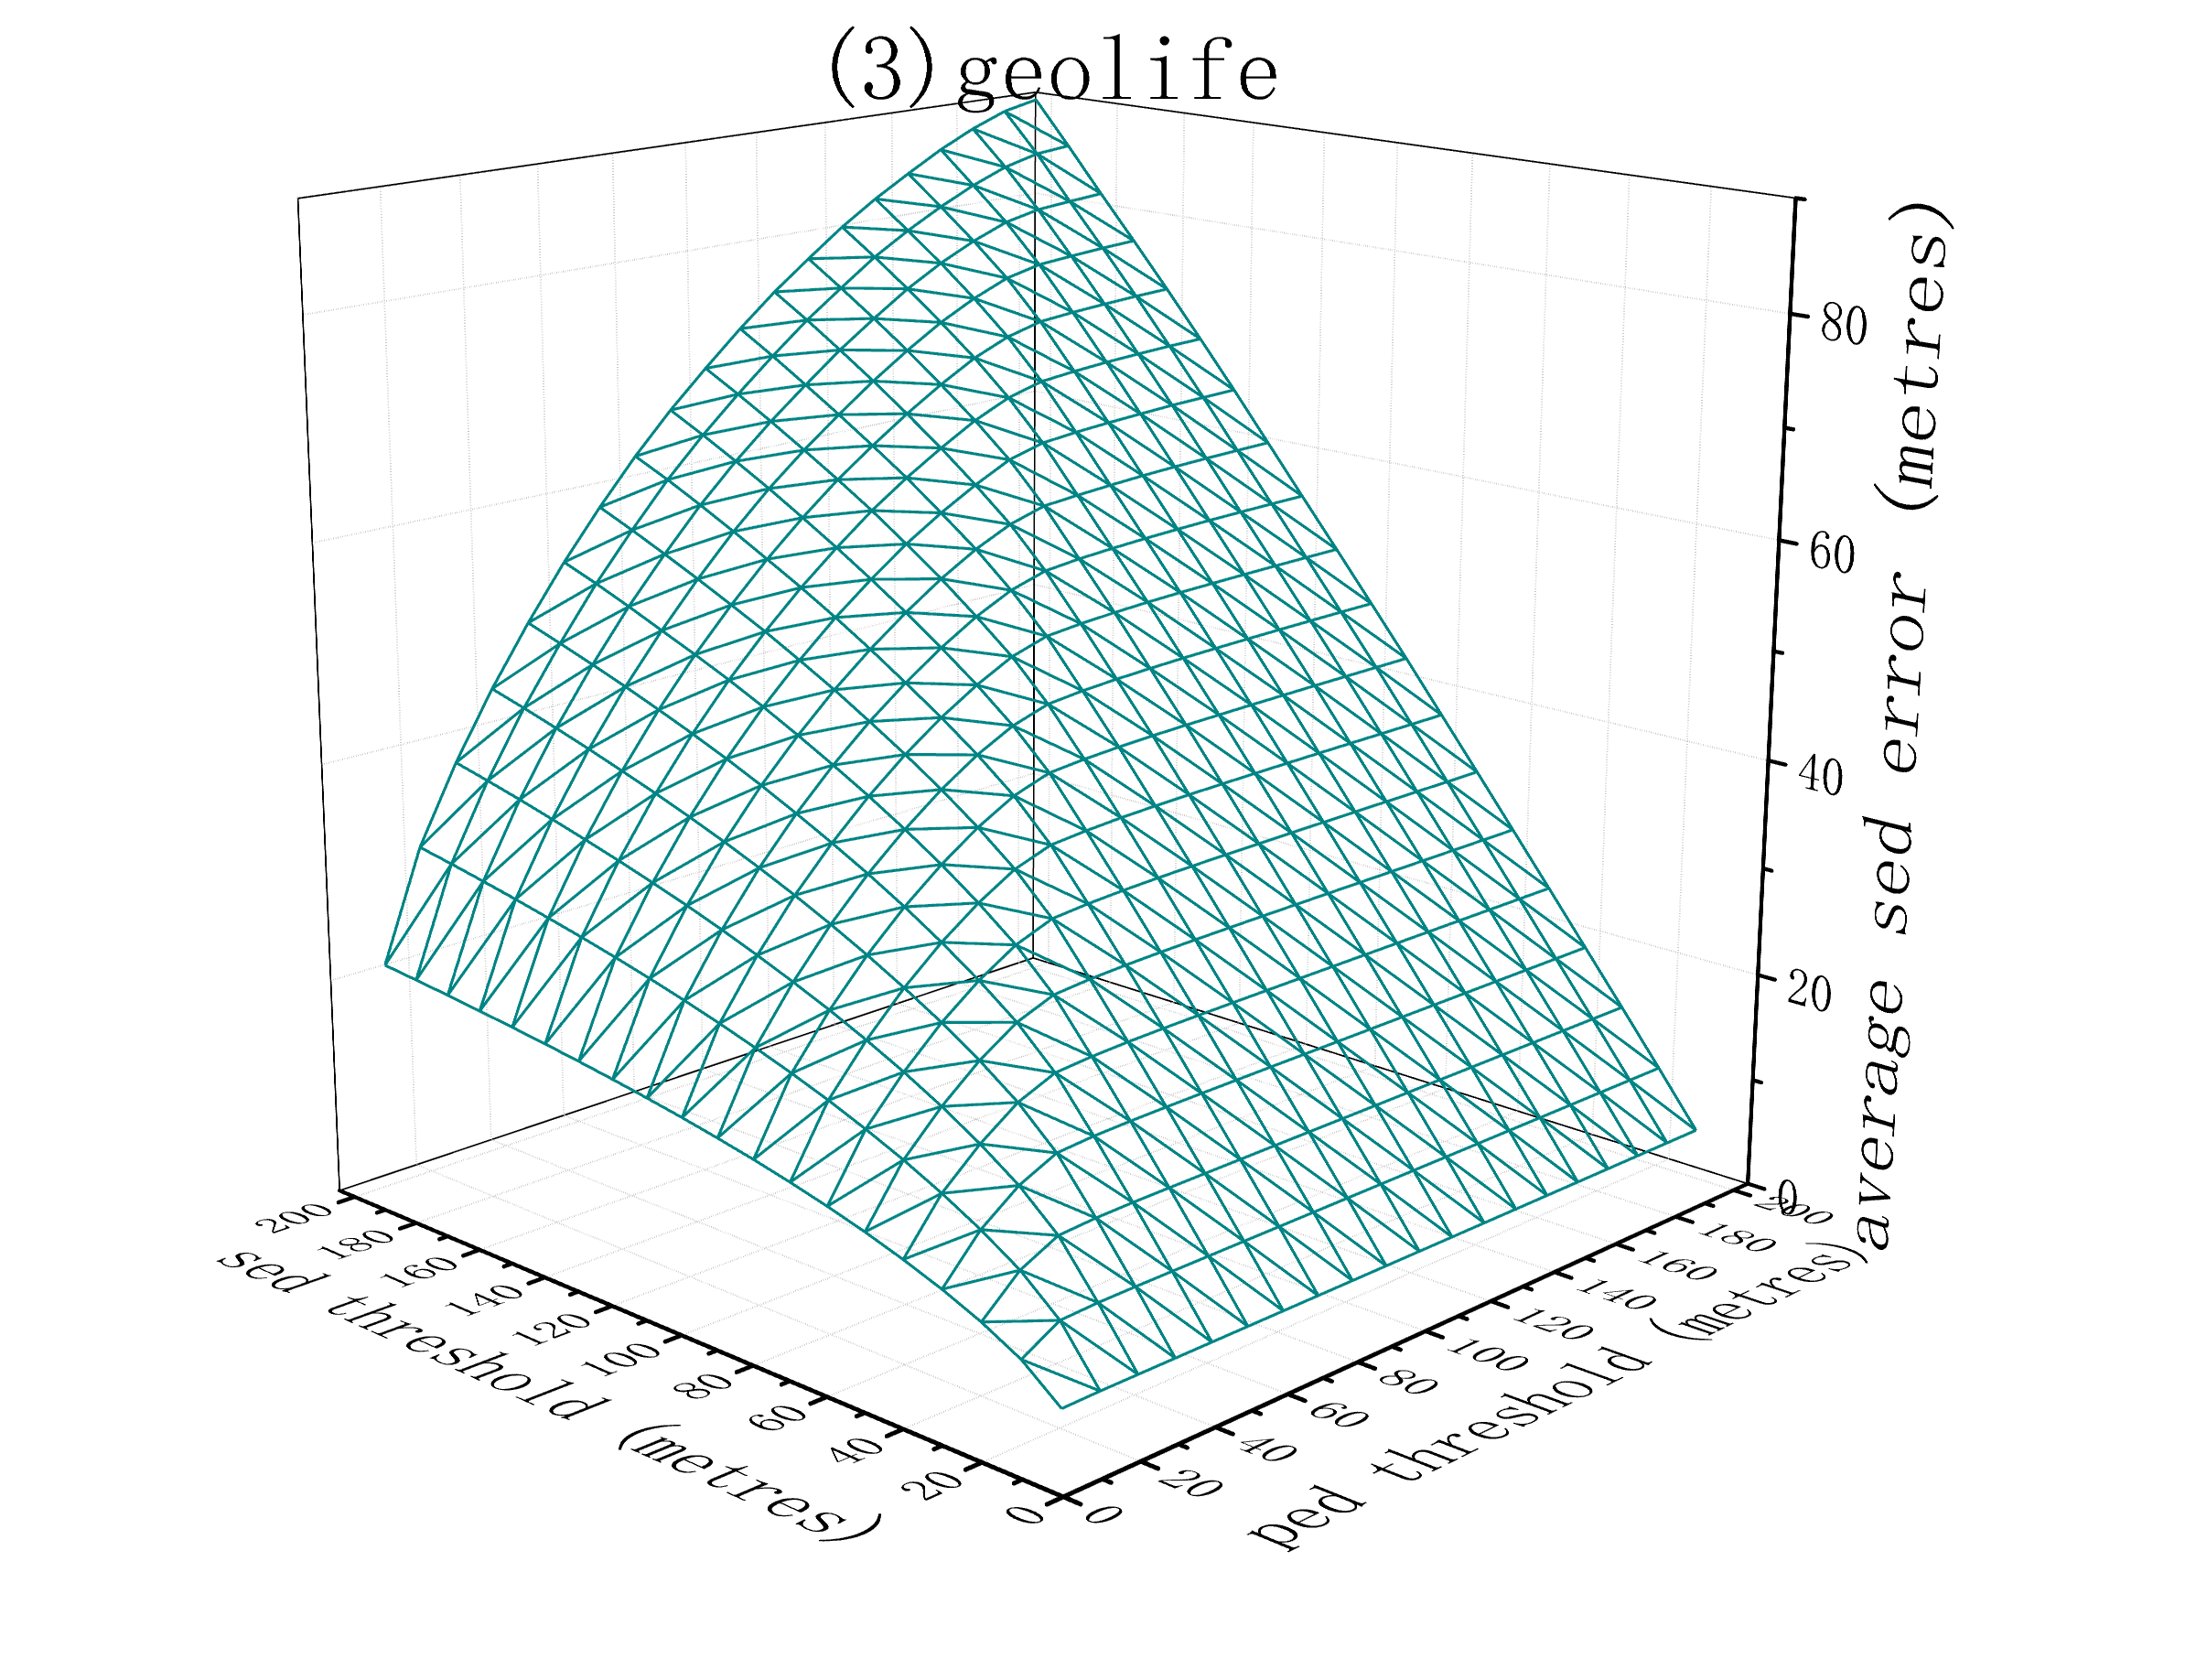
\includegraphics[scale = 0.210]{figures/Fig-BITT-geolife-sed-error.png}\hspace{1ex}
	%\vspace{-1ex}
	\caption{\small Evaluation of BITT sed error: varying error bounds $\epsilon_{sed}$ and $\epsilon_{ped}$.}
	\label{fig:bitt-sed-error}
	%\vspace{-1ex}
\end{figure*}



\begin{figure*}[tb!]
	\centering
	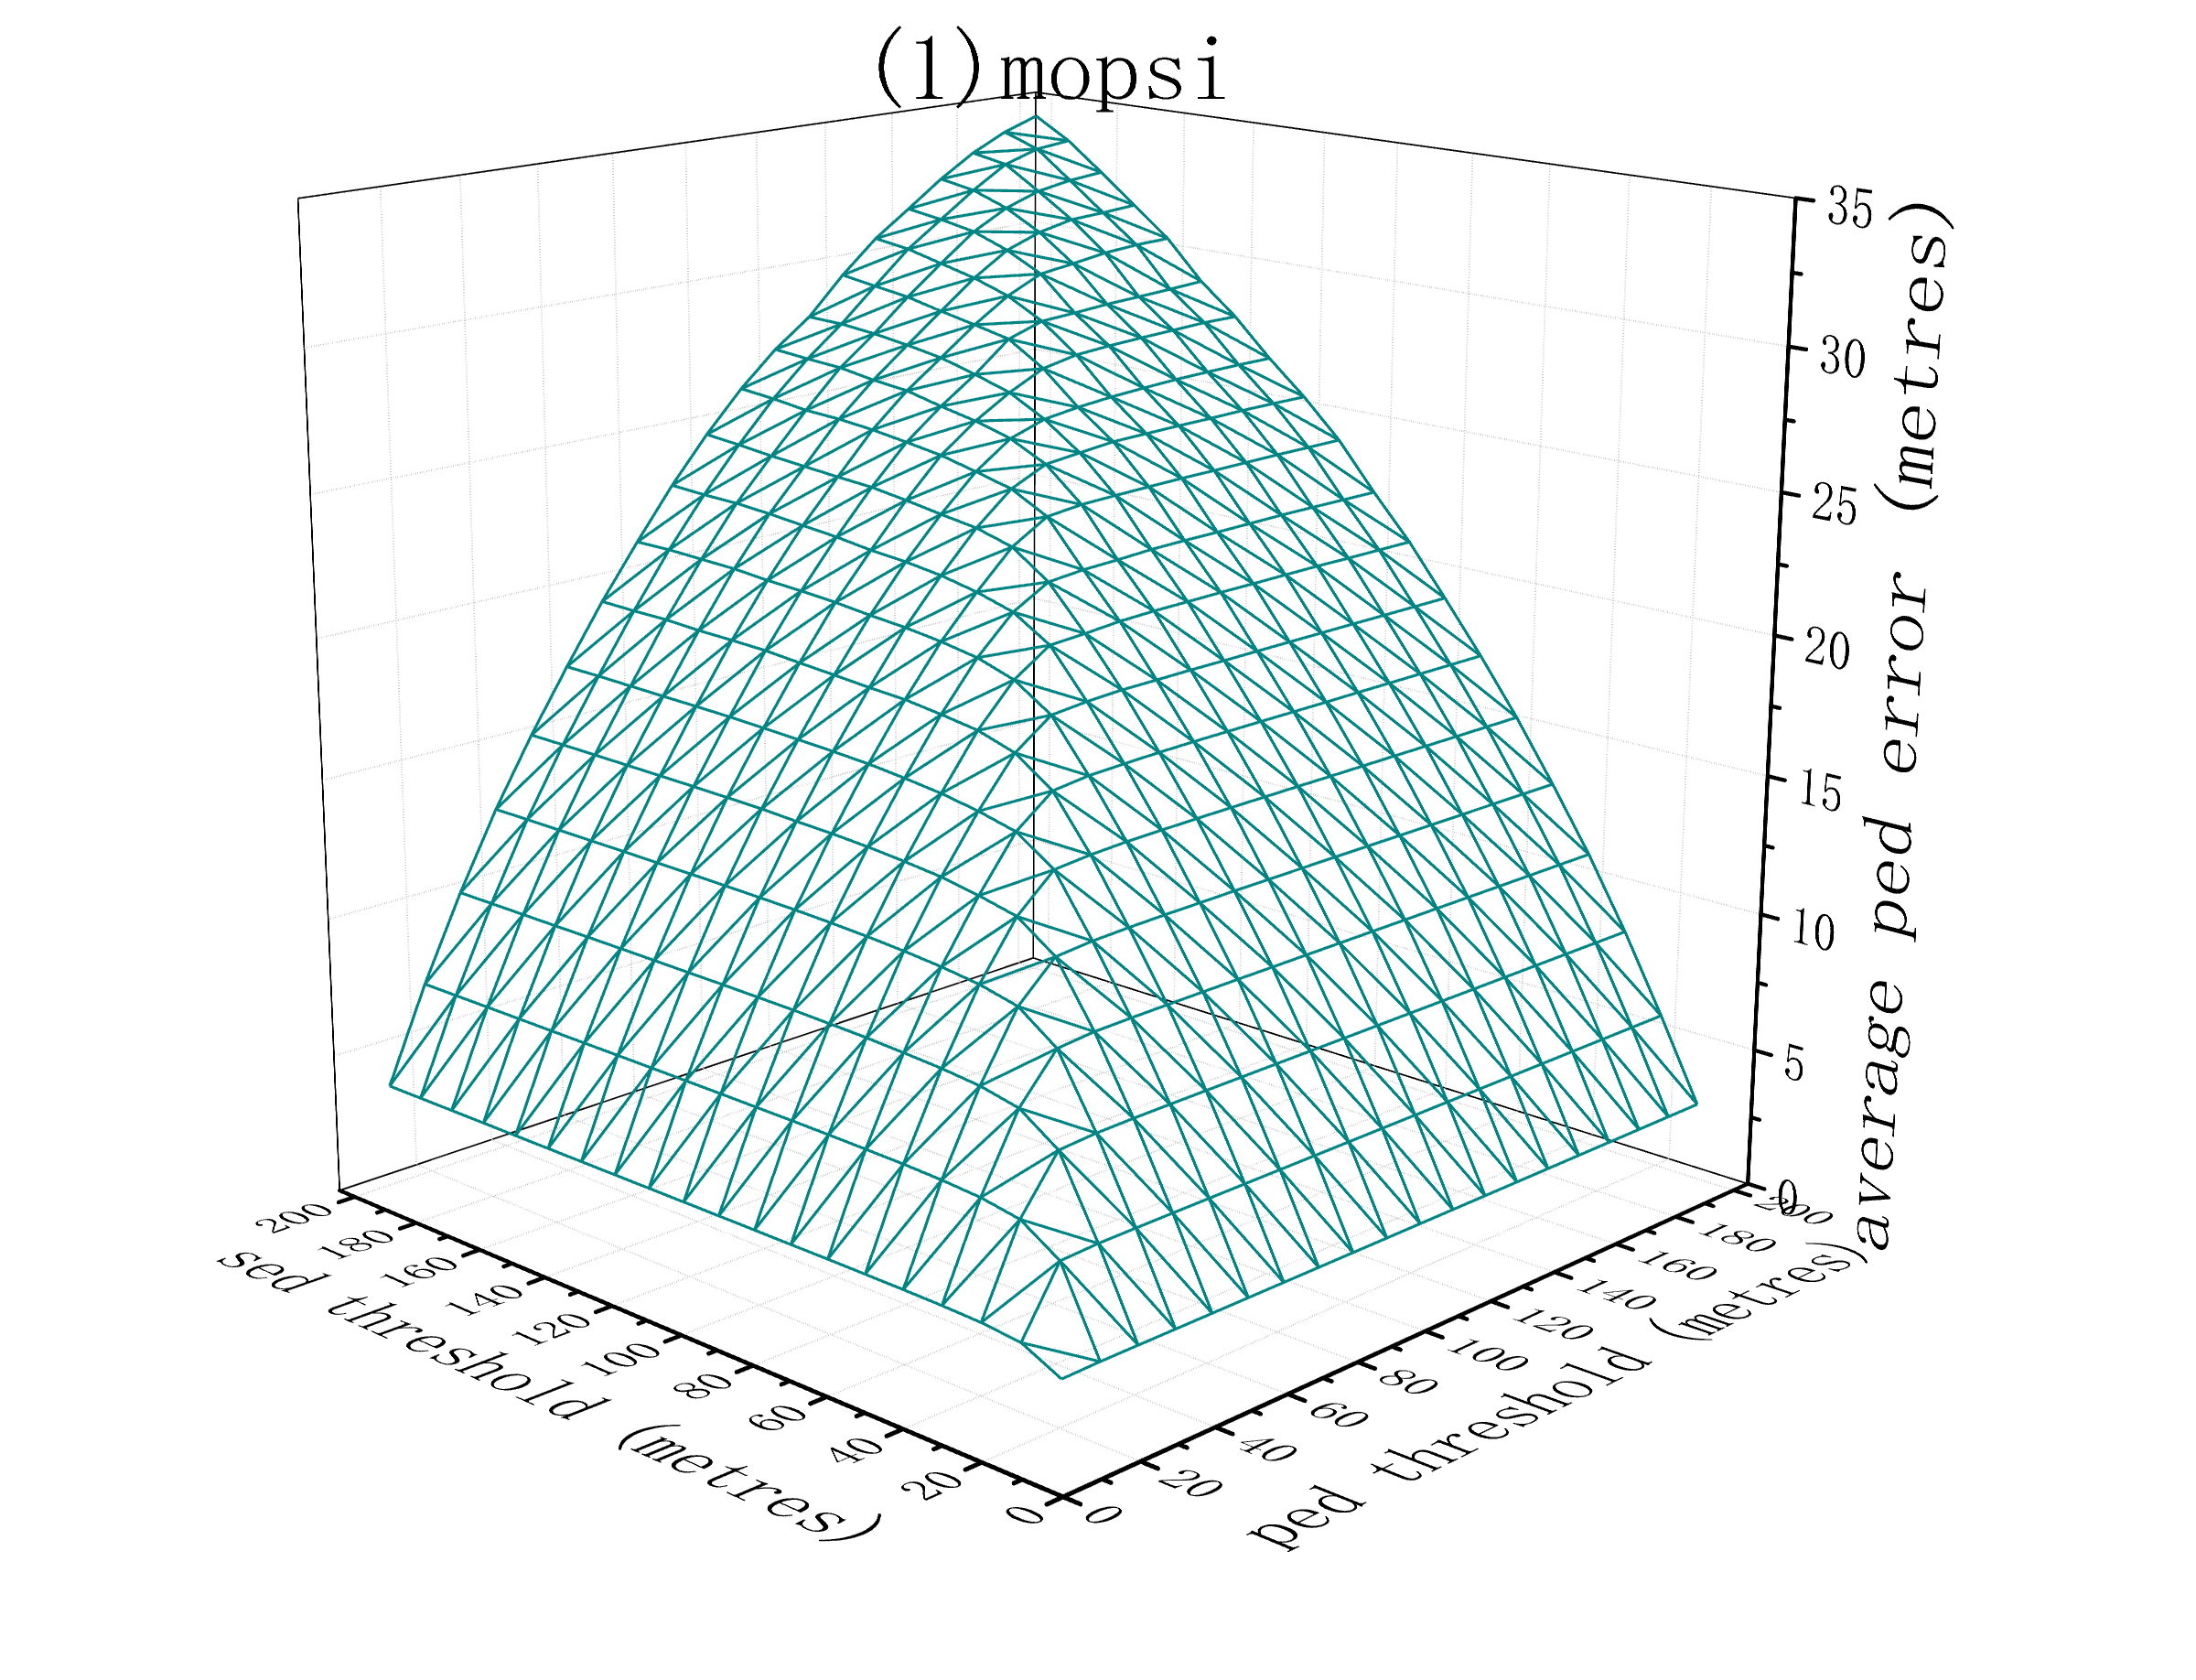
\includegraphics[scale = 0.210]{figures/Fig-BITT-mopsi-ped-error.png}\hspace{1ex}
	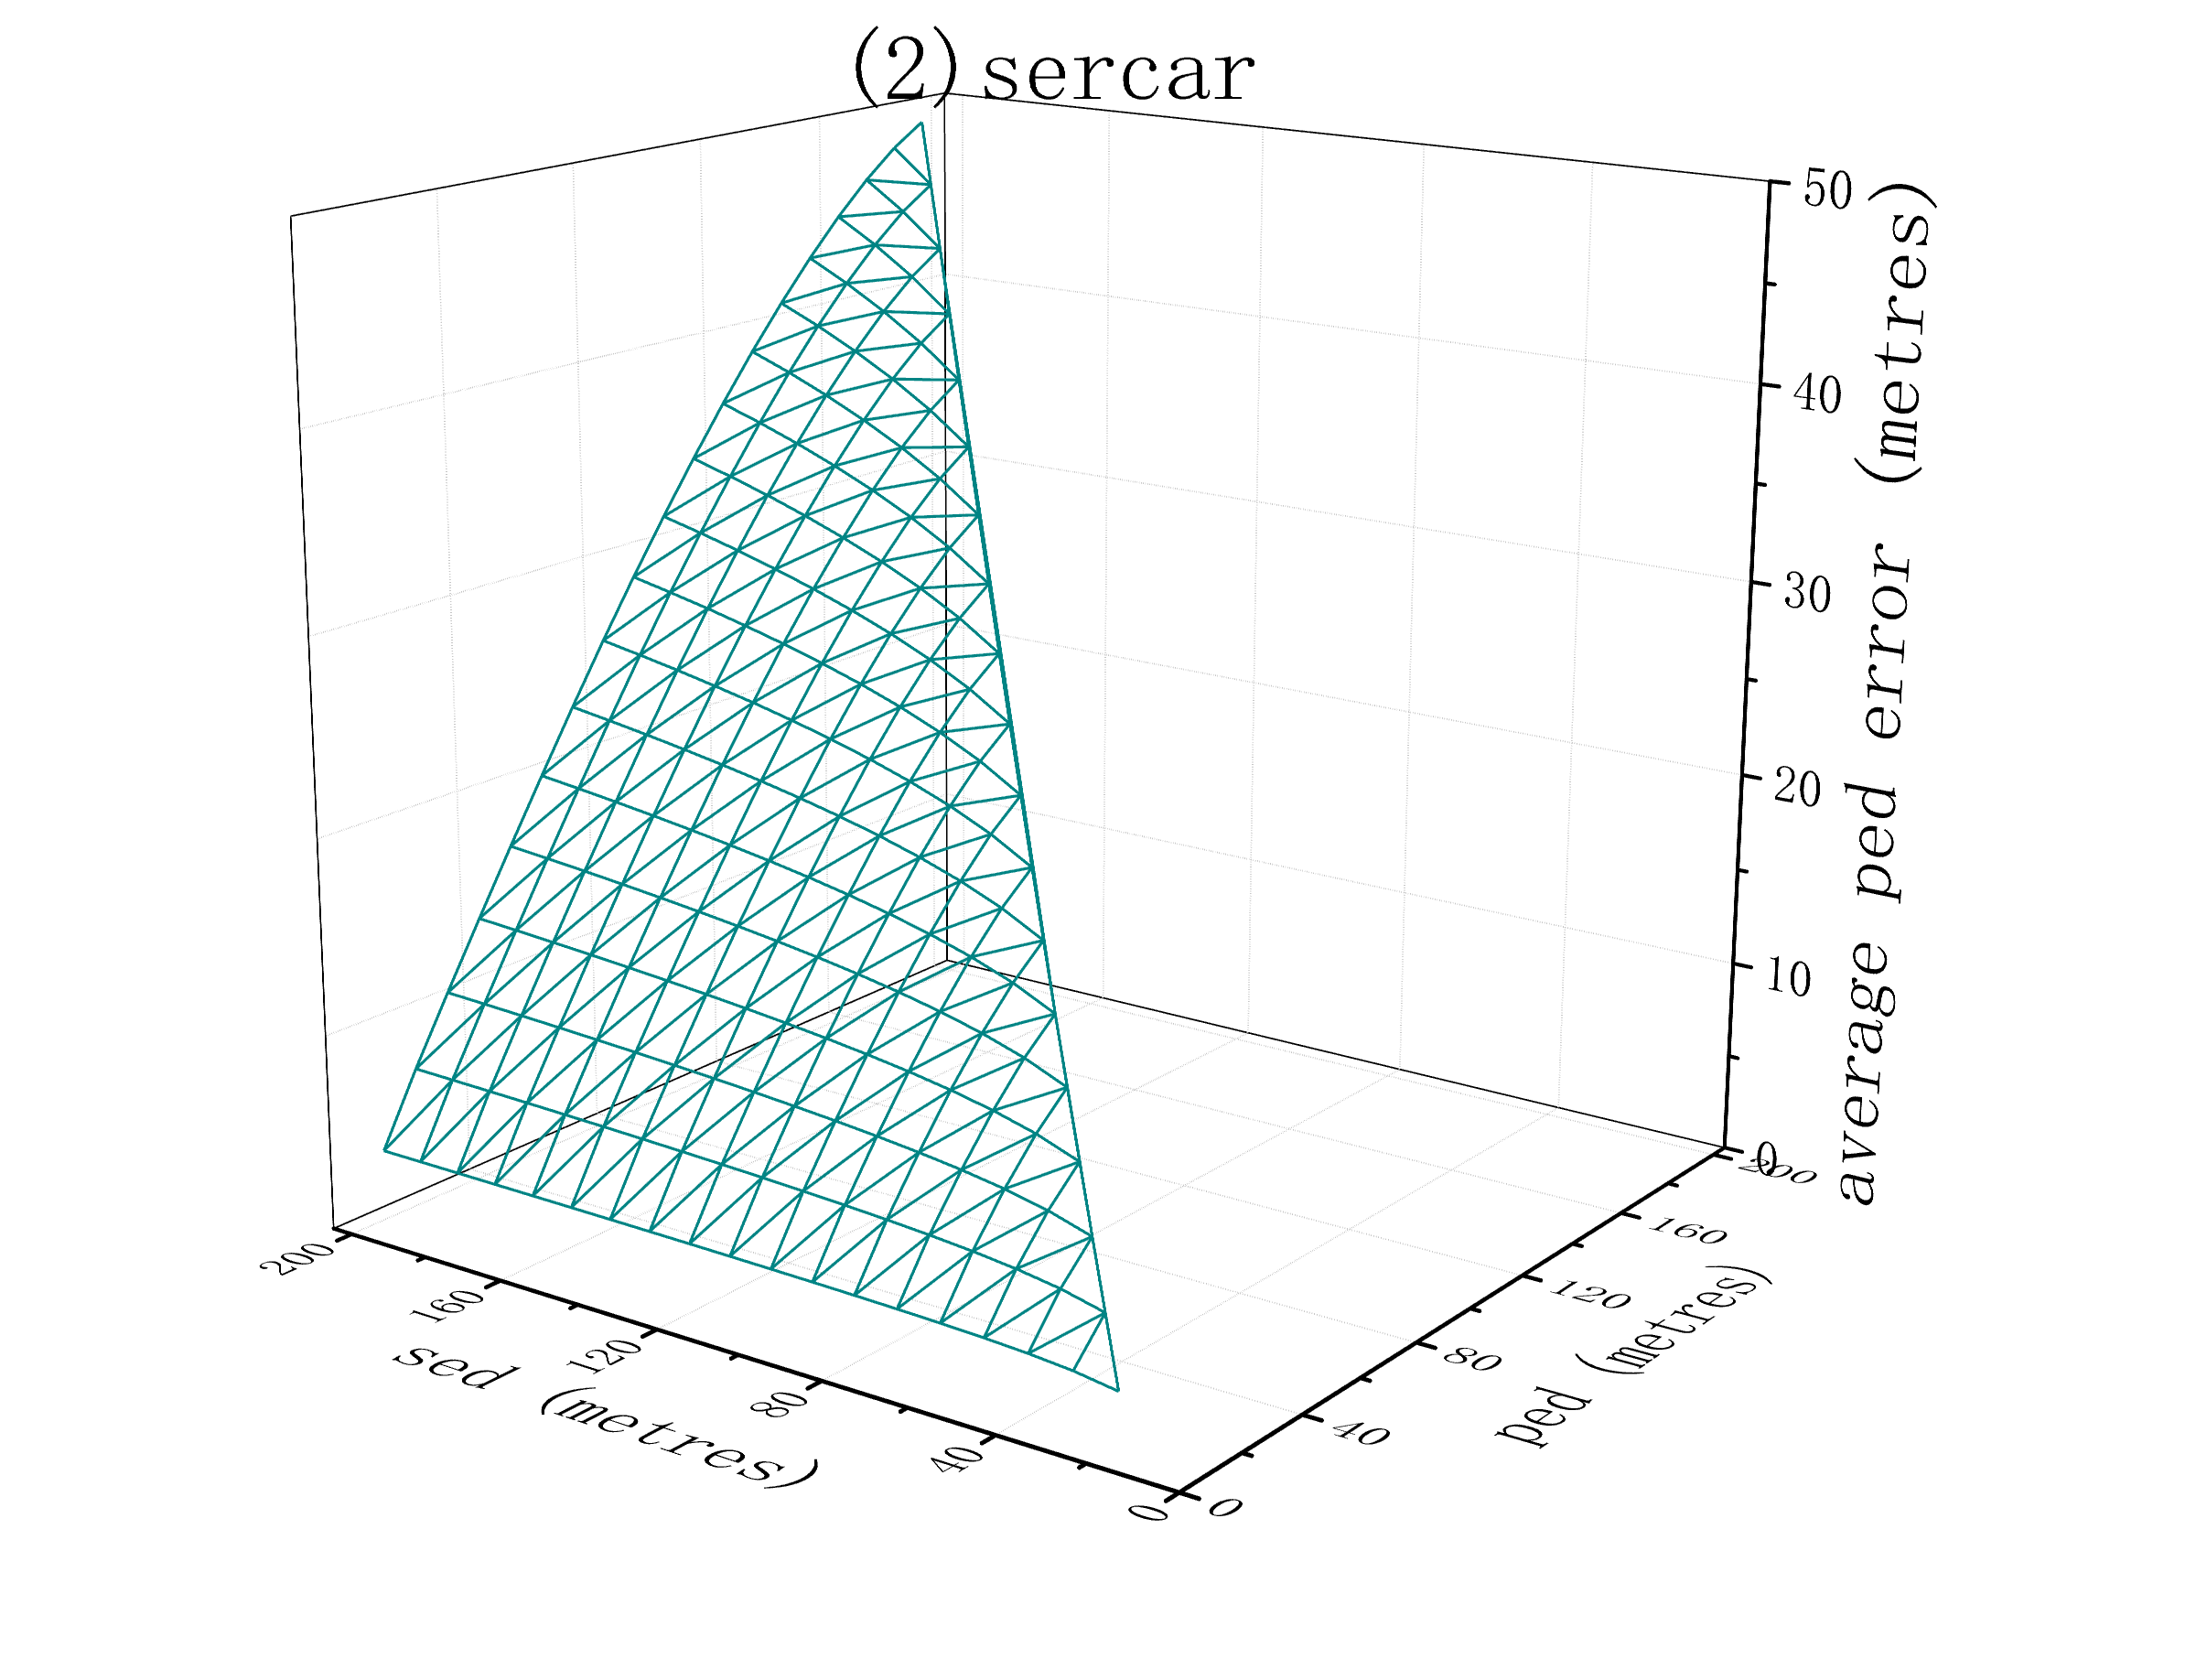
\includegraphics[scale = 0.210]{figures/Fig-BITT-sercar-ped-error.png}\hspace{1ex}
	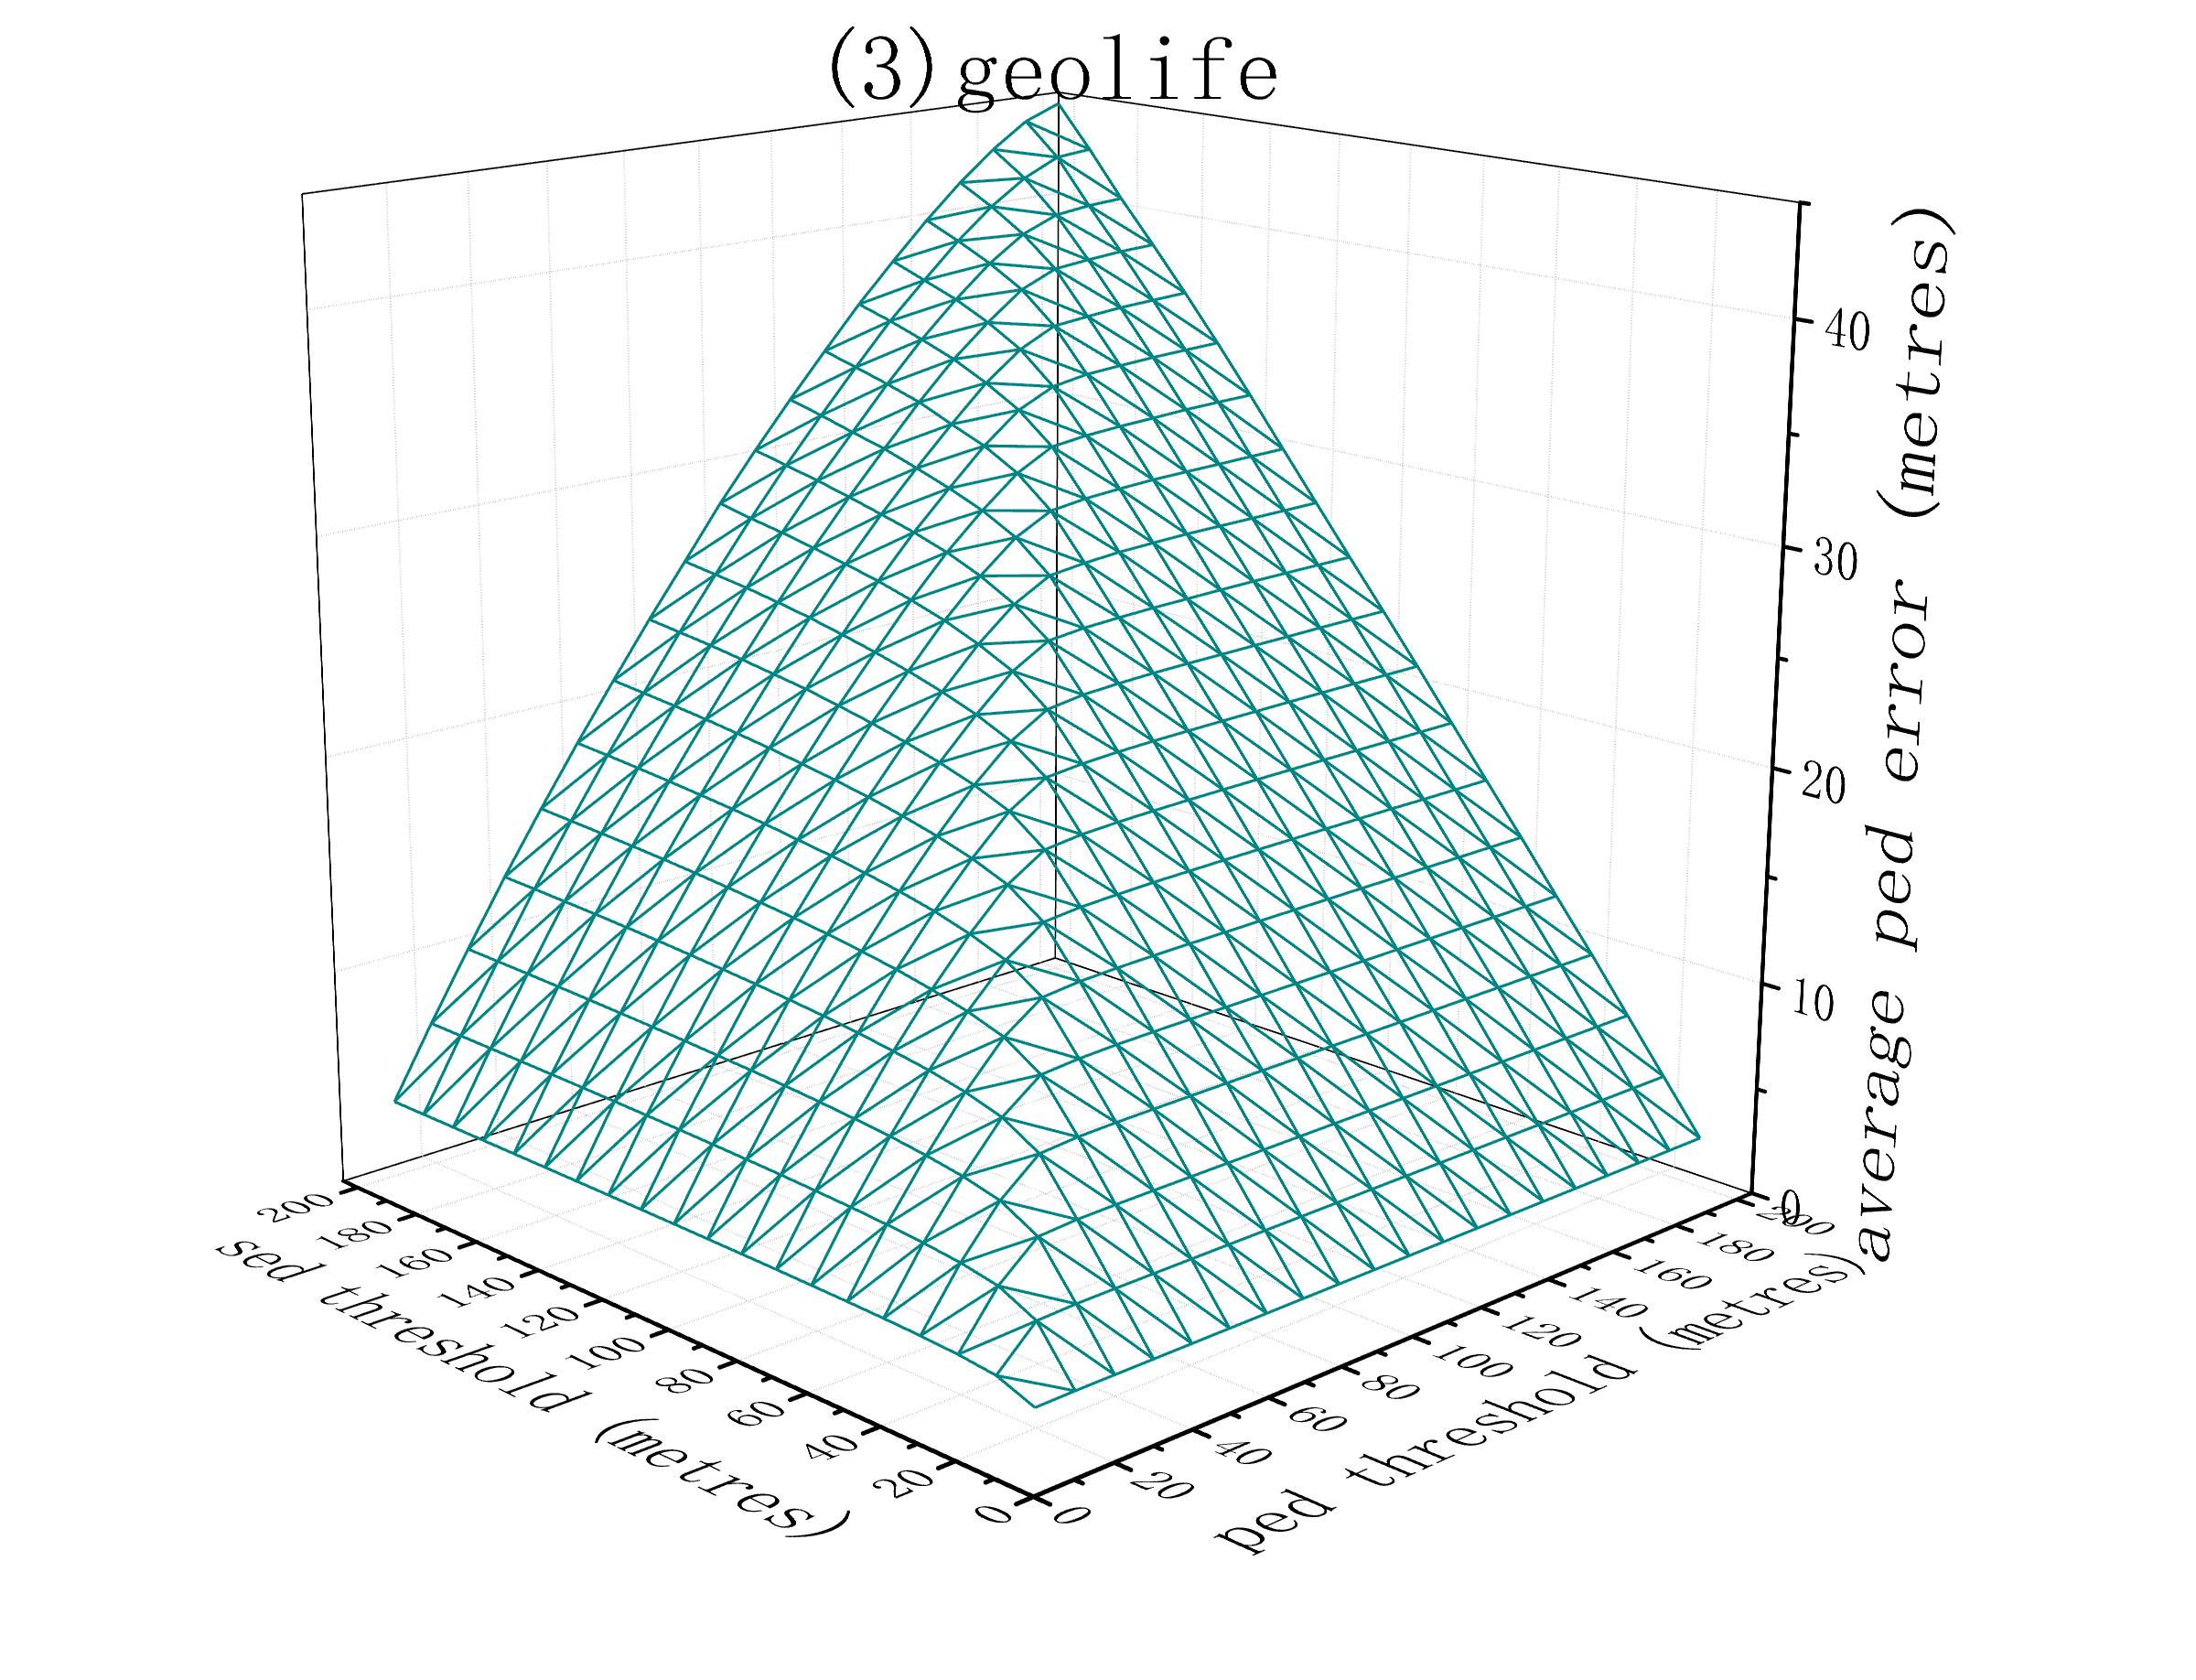
\includegraphics[scale = 0.210]{figures/Fig-BITT-geolife-ped-error.png}\hspace{1ex}
	%\vspace{-1ex}
	\caption{\small Evaluation of BITT ped error: varying error bounds $\epsilon_{sed}$ and $\epsilon_{ped}$.}
	\label{fig:bitt-ped-error}
	%\vspace{-1ex}
\end{figure*}





\subsubsection{Comparing \bitt, \sitt and \citt with \ldrh and \grts.}
This section compares our algorithms \citt, \sitt and \bitt with algorithms \ldrh and \grts.
We varied the error bound (either $\epsilon_{sed}$ or $\epsilon_{ped}$) from $10$ meters to $200$ meters on the entire three datasets, respectively. 
\myred{For \bitt, the we fixed $\epsilon_{ped}$ used by \bitt is 0.9 times the $\epsilon_{ped}$ used by \sitt, and the $\epsilon_{sed}$ is 1.7 times the $\epsilon_{sed}$ used by \citt, \grts and \ldrh.}
%
The results are reported in Figures~\ref{fig:total-message}, \ref{fig:speed-message},\ref{fig:compression-ratio}, \ref{fig:sed-error}, \ref{fig:ped-error} and \ref{fig:running-time}.


\begin{figure*}[tb!]
	\centering
	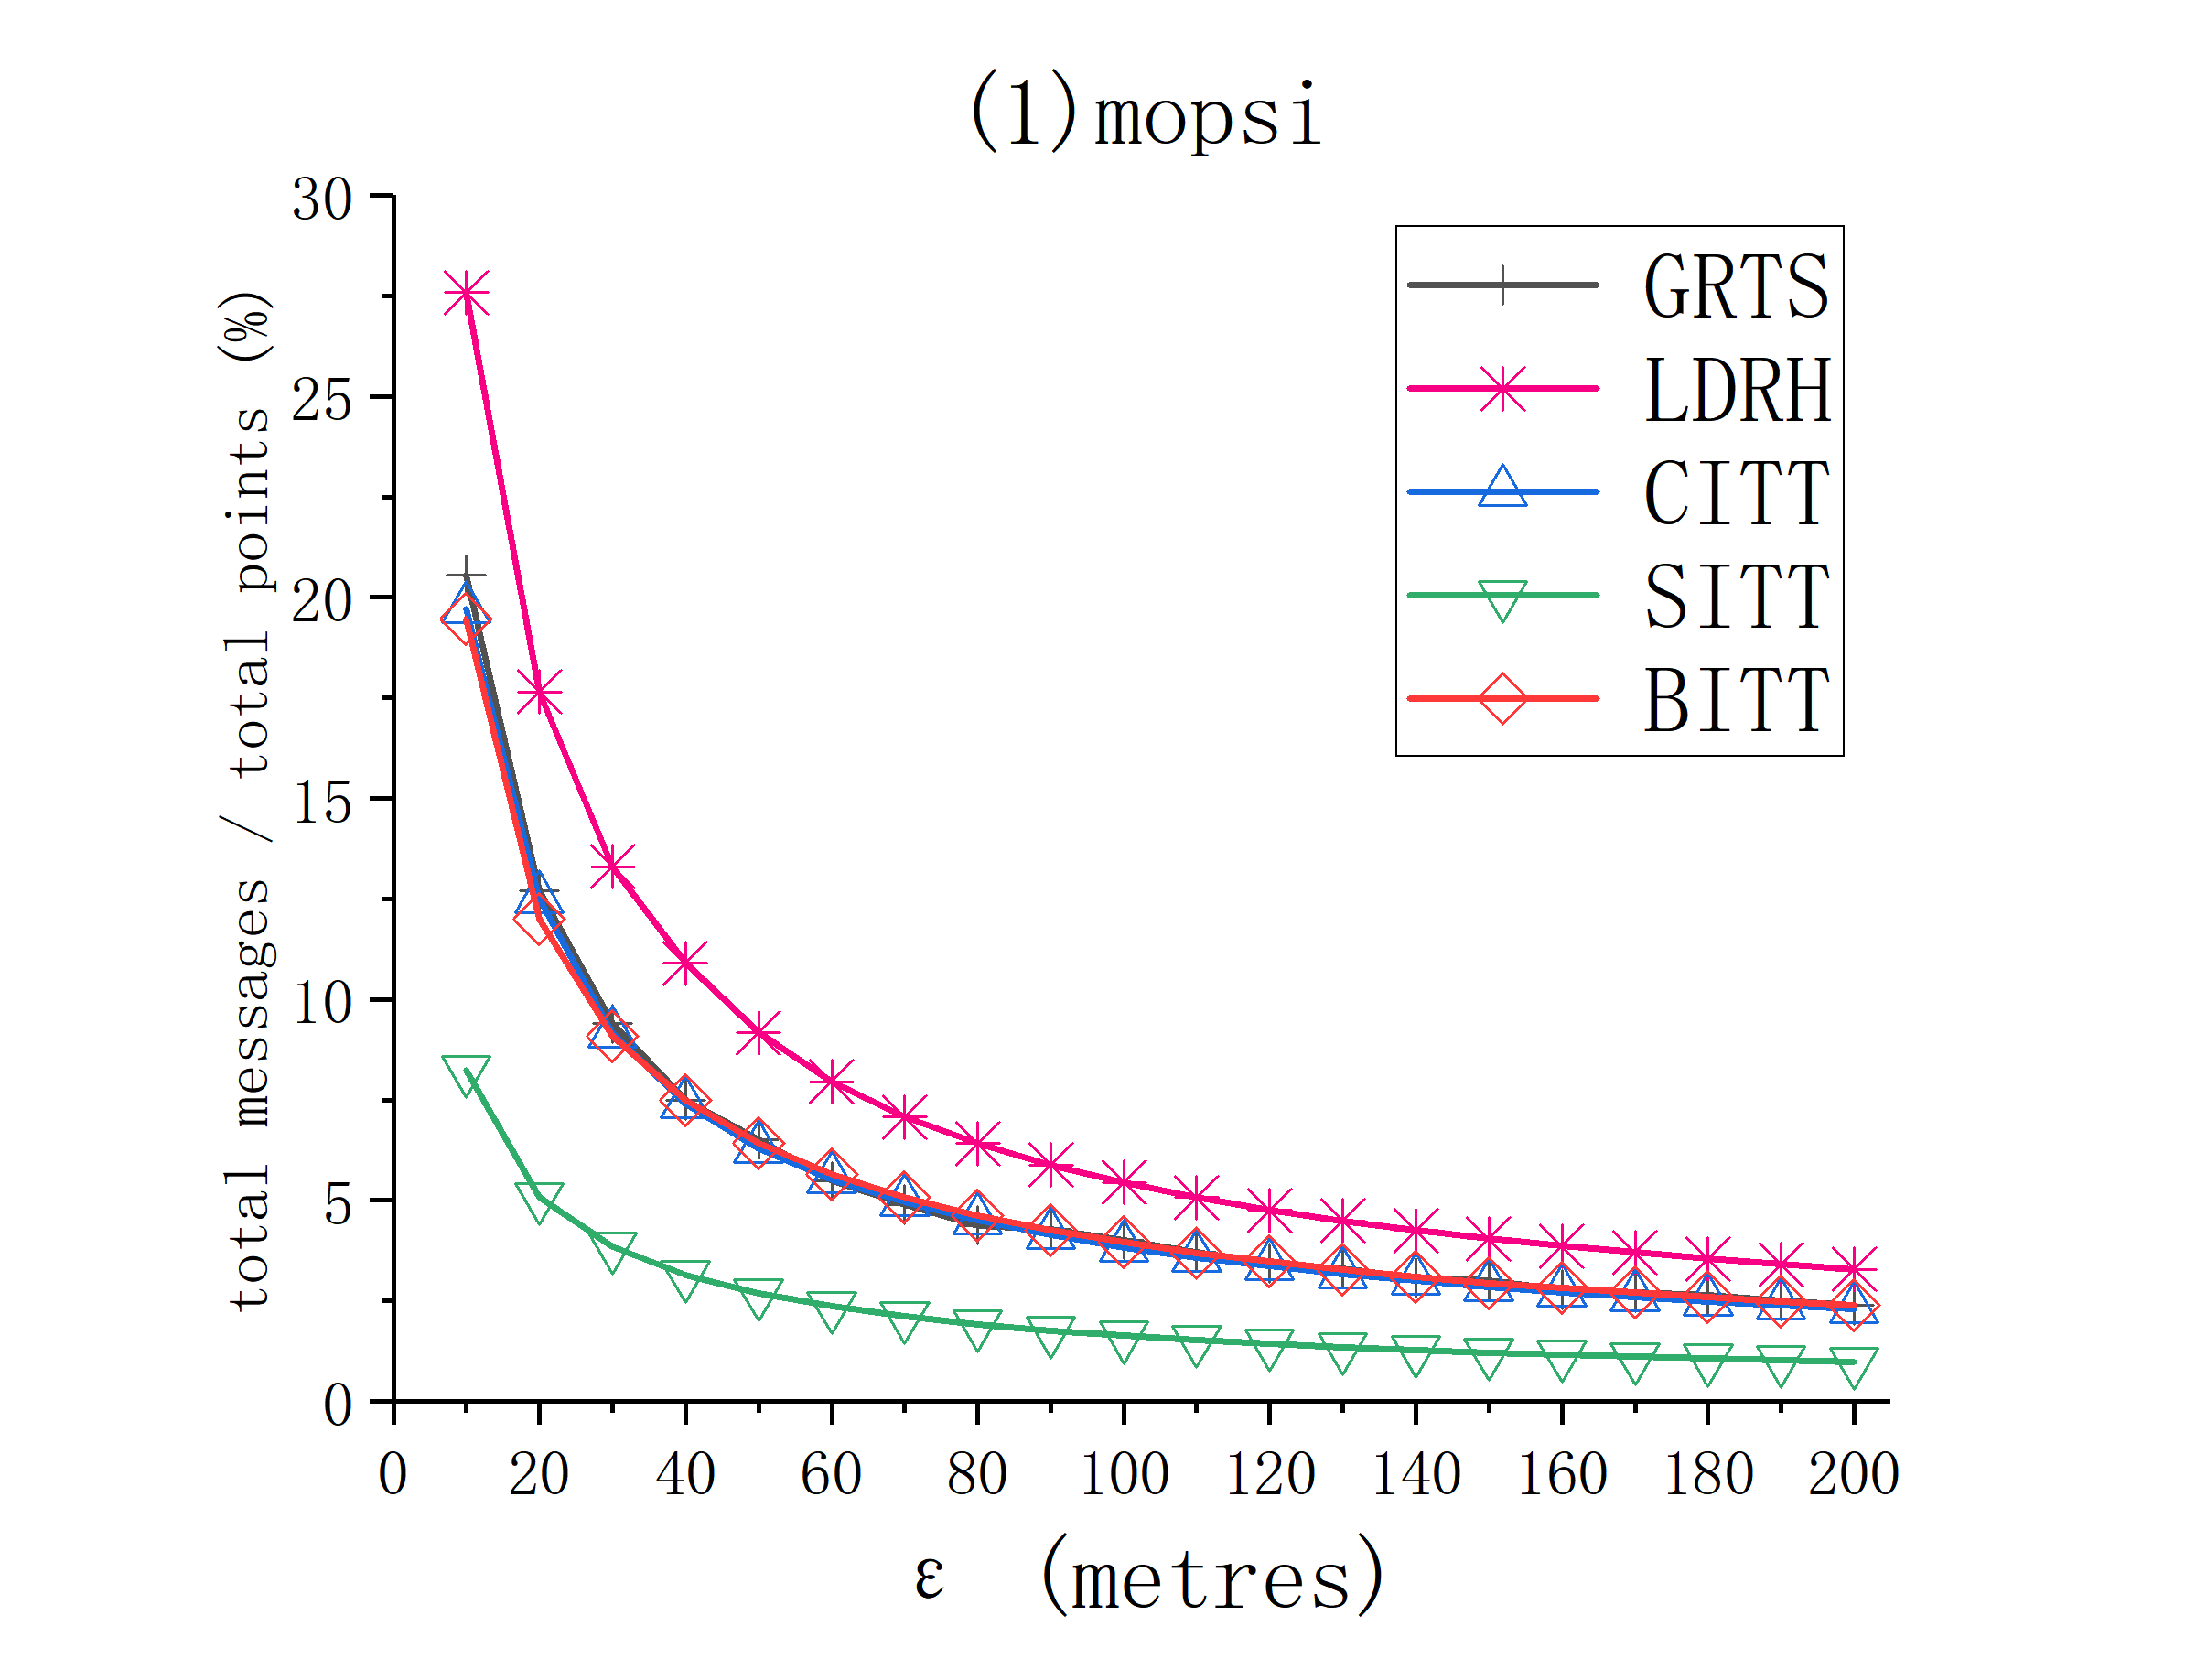
\includegraphics[scale = 0.210]{figures/Fig-mopsi-total-messages.png}\hspace{1ex}
	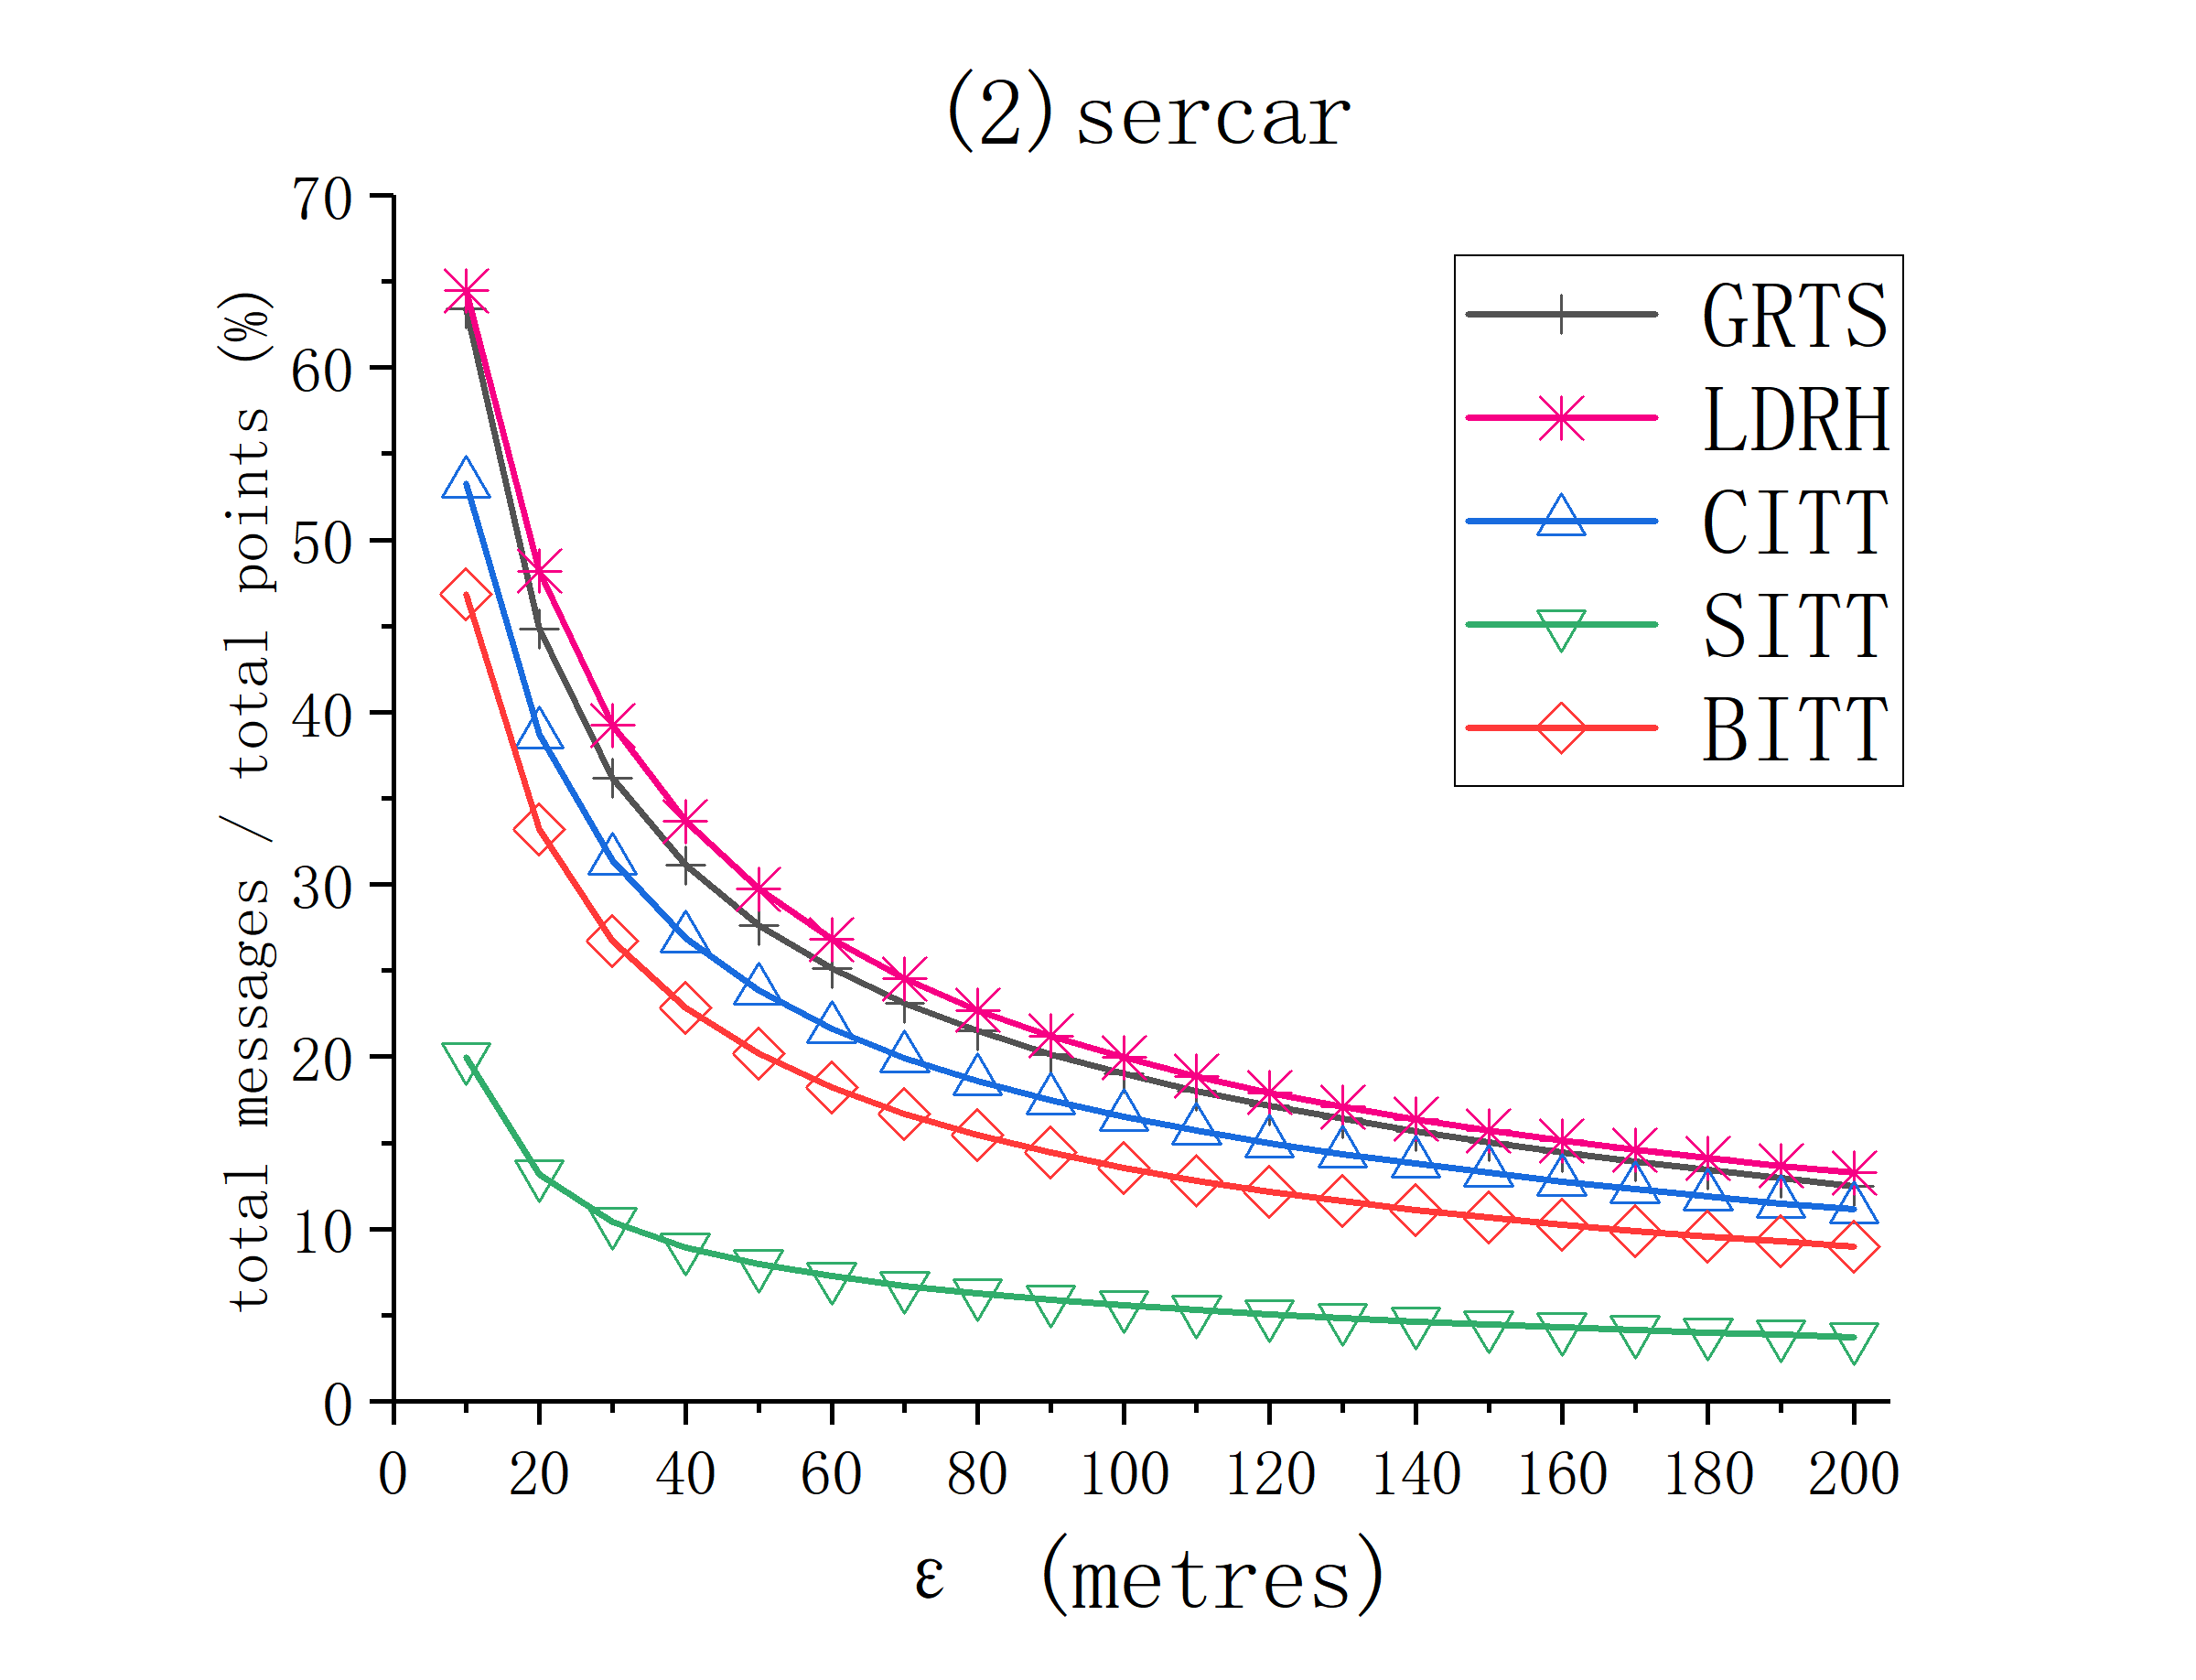
\includegraphics[scale = 0.210]{figures/Fig-sercar-total-messages.png}\hspace{1ex}
	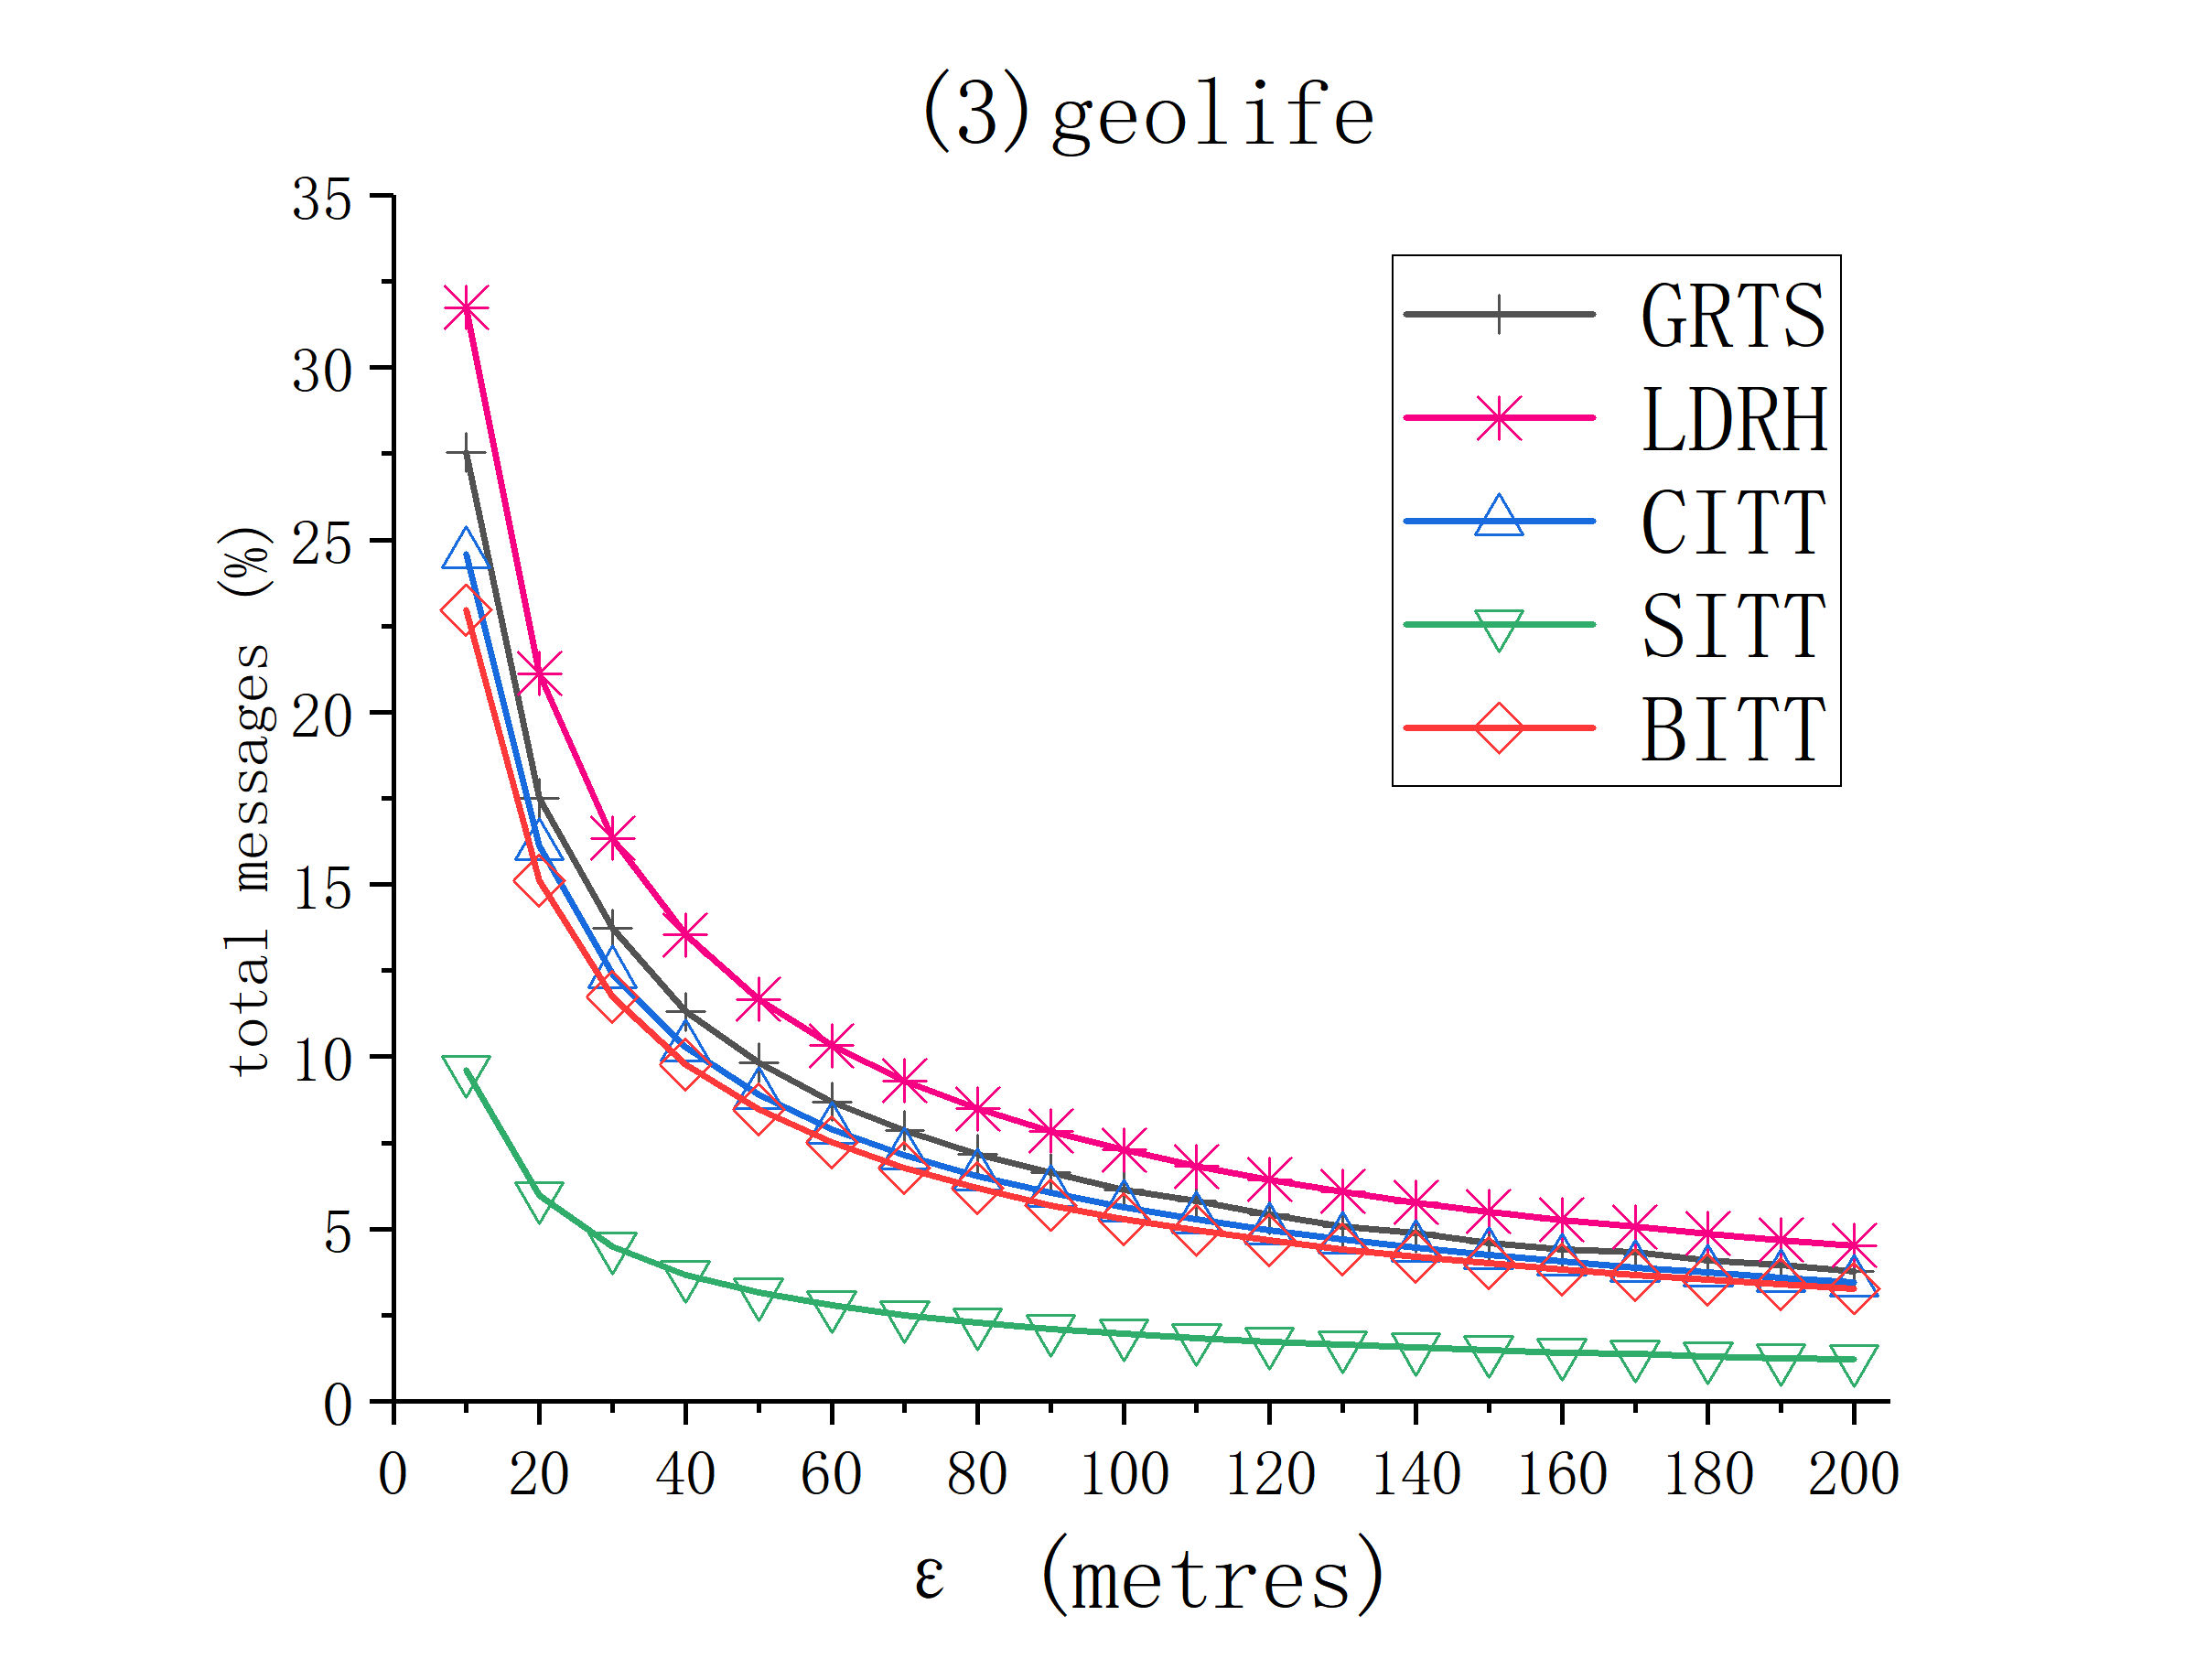
\includegraphics[scale = 0.210]{figures/Fig-geolife-total-messages.png}\hspace{1ex}
	%\vspace{-1ex}
	\caption{\small Evaluation of total messages: varying error bounds $\epsilon_{sed}$ and $\epsilon_{ped}$.}
	\label{fig:total-message}
	%\vspace{-1ex}
\end{figure*}

\begin{figure*}[tb!]
	\centering
	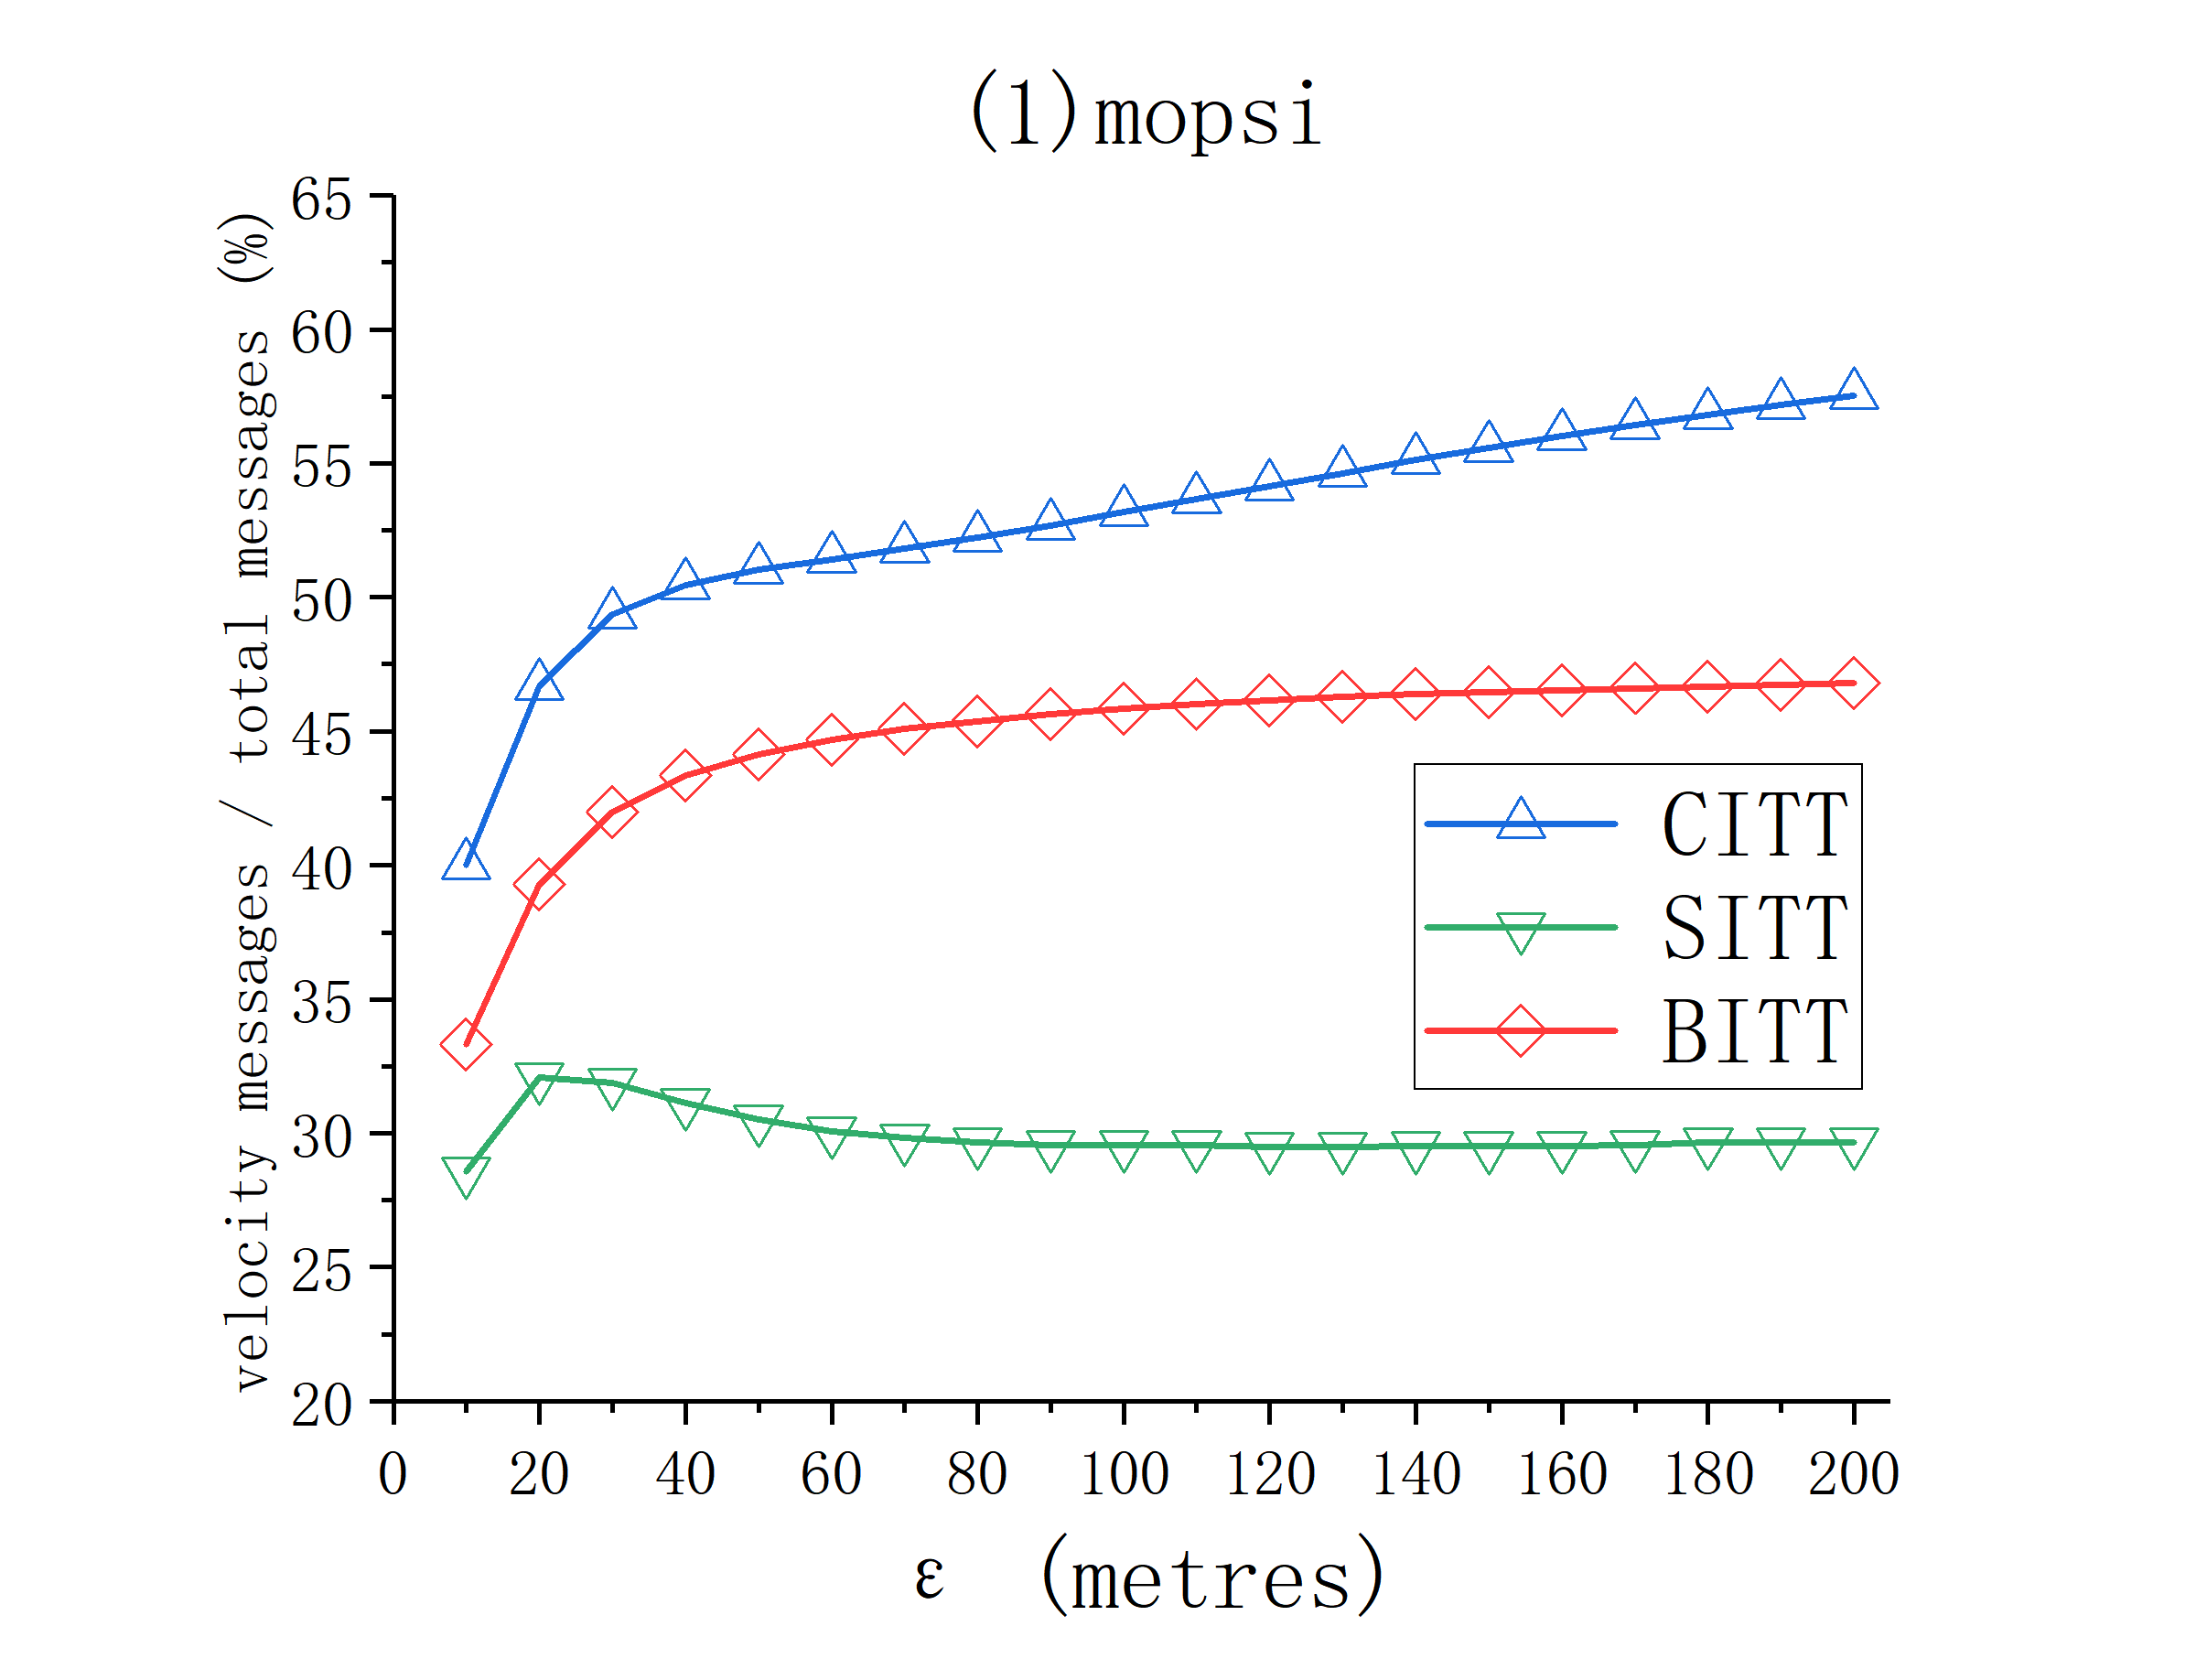
\includegraphics[scale = 0.210]{figures/Fig-mopsi-speed-messages.png}\hspace{1ex}
	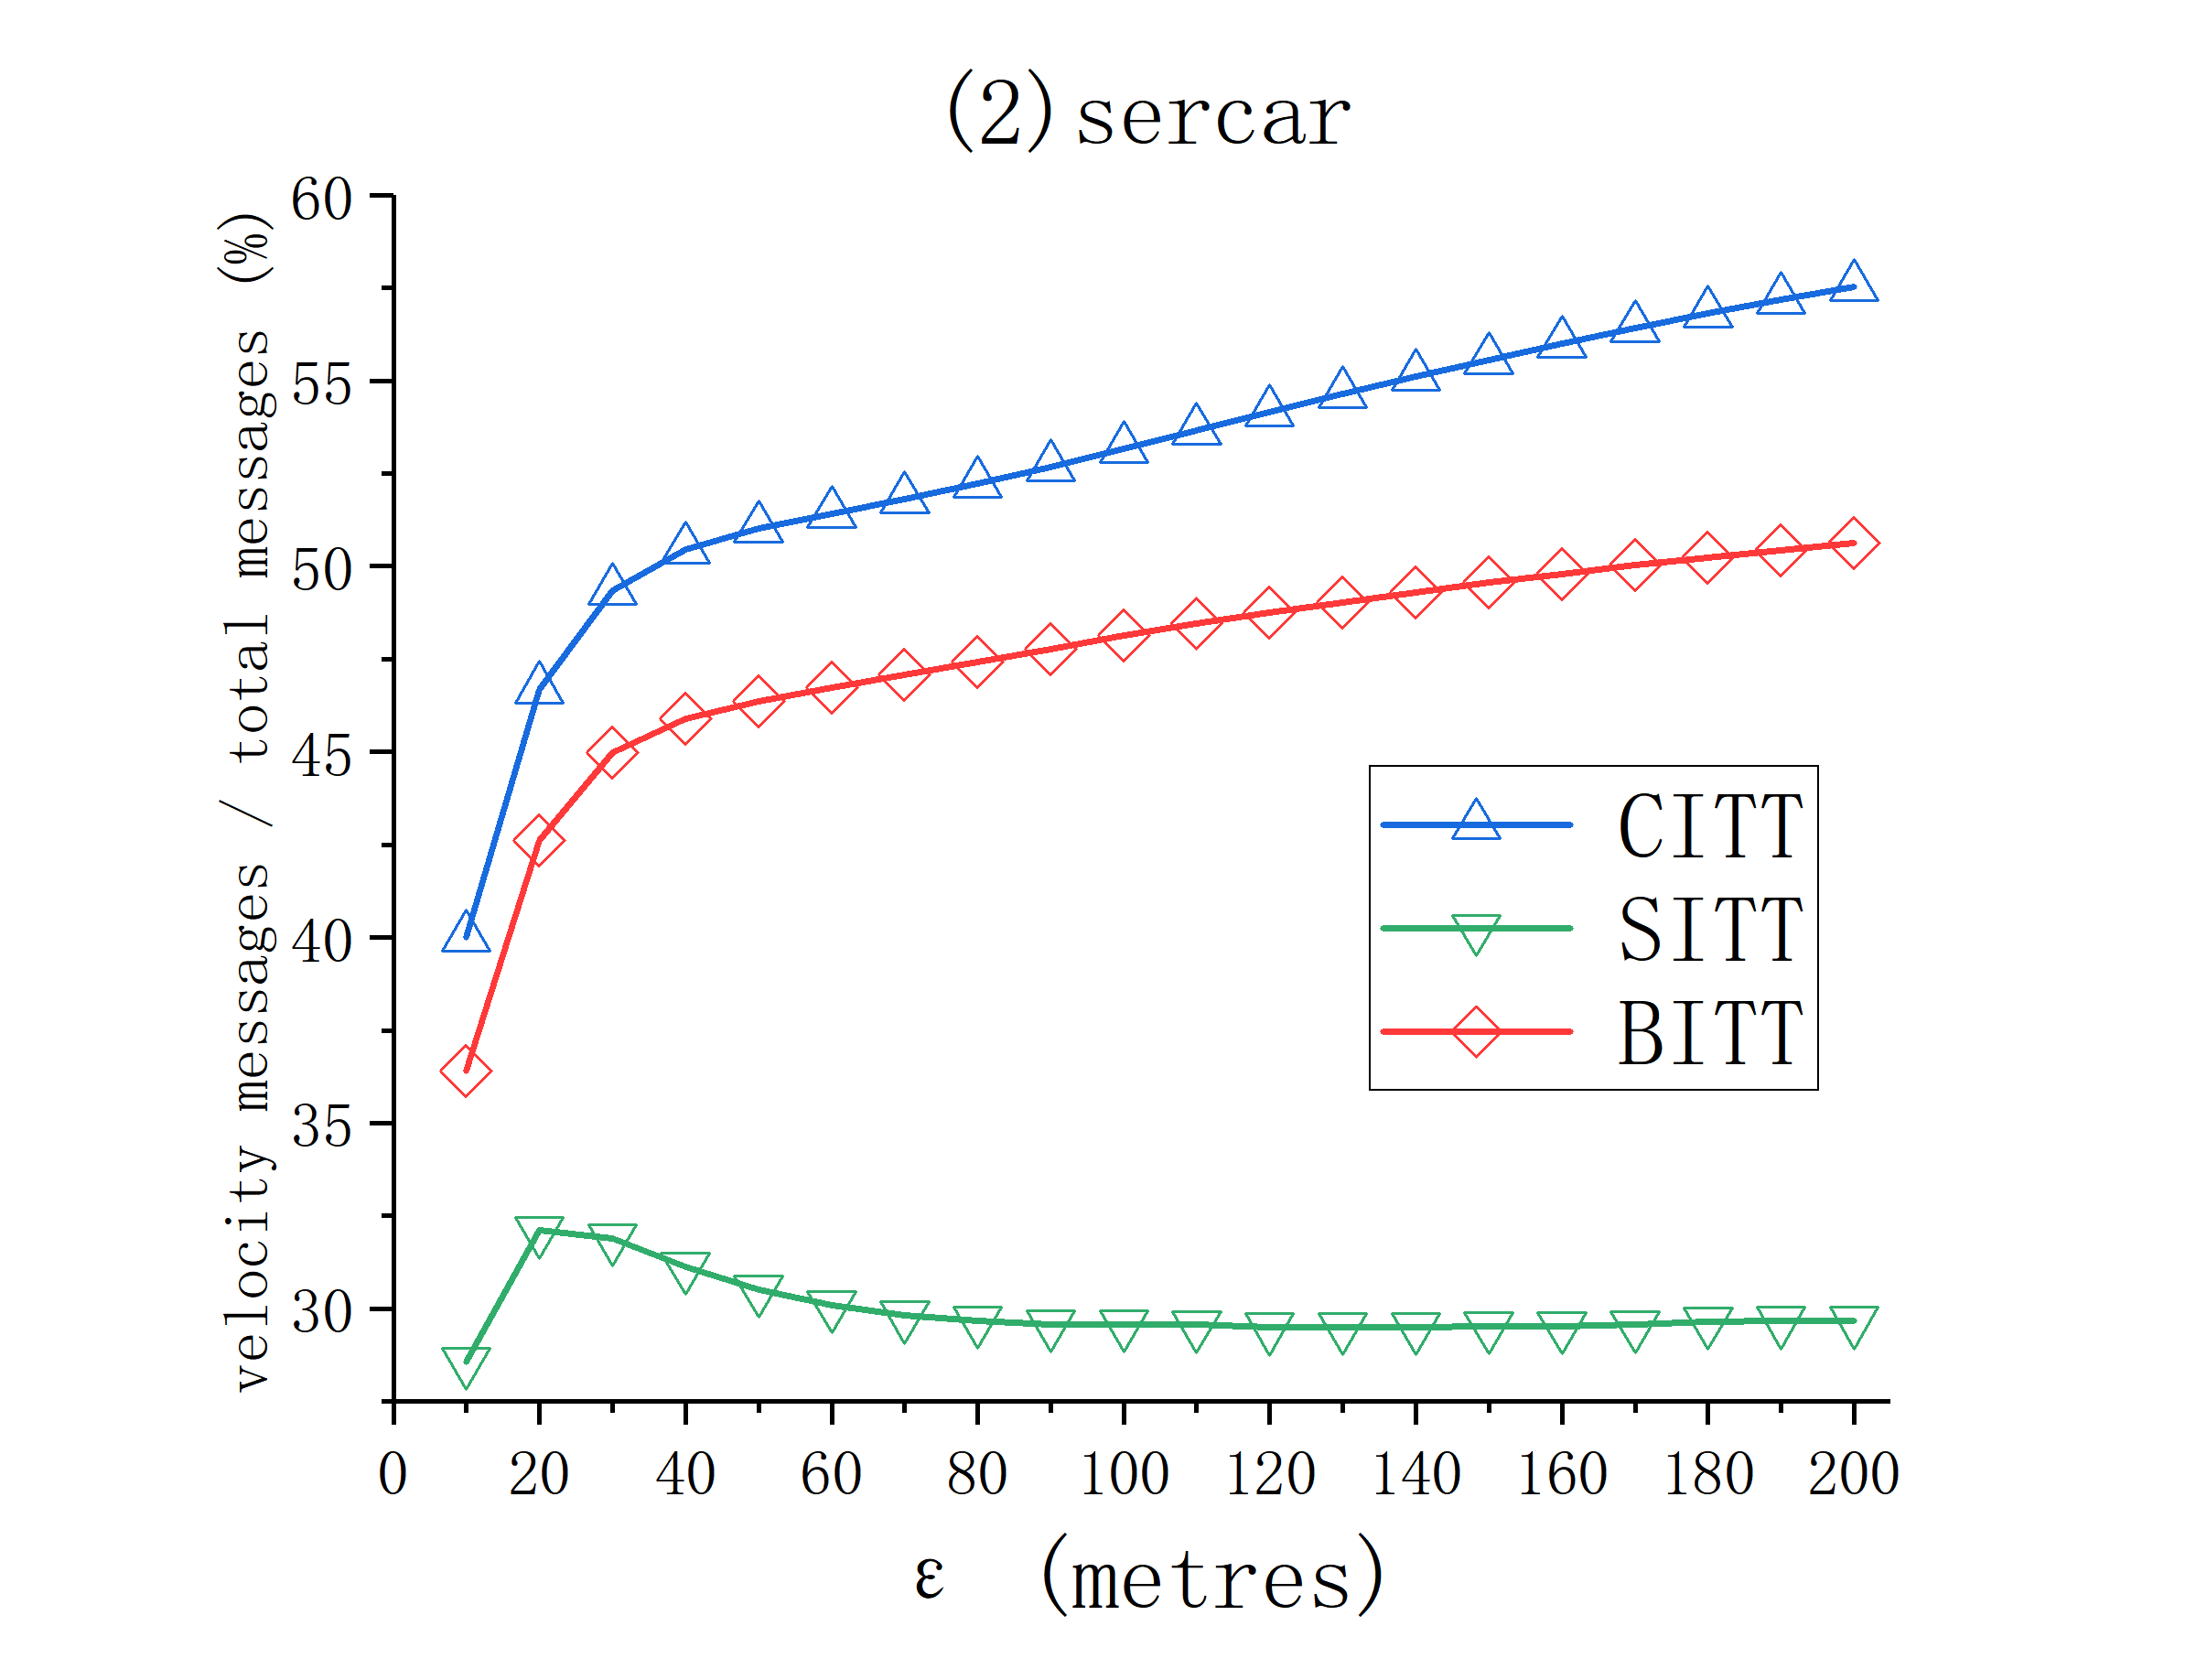
\includegraphics[scale = 0.210]{figures/Fig-sercar-speed-messages.png}\hspace{1ex}
	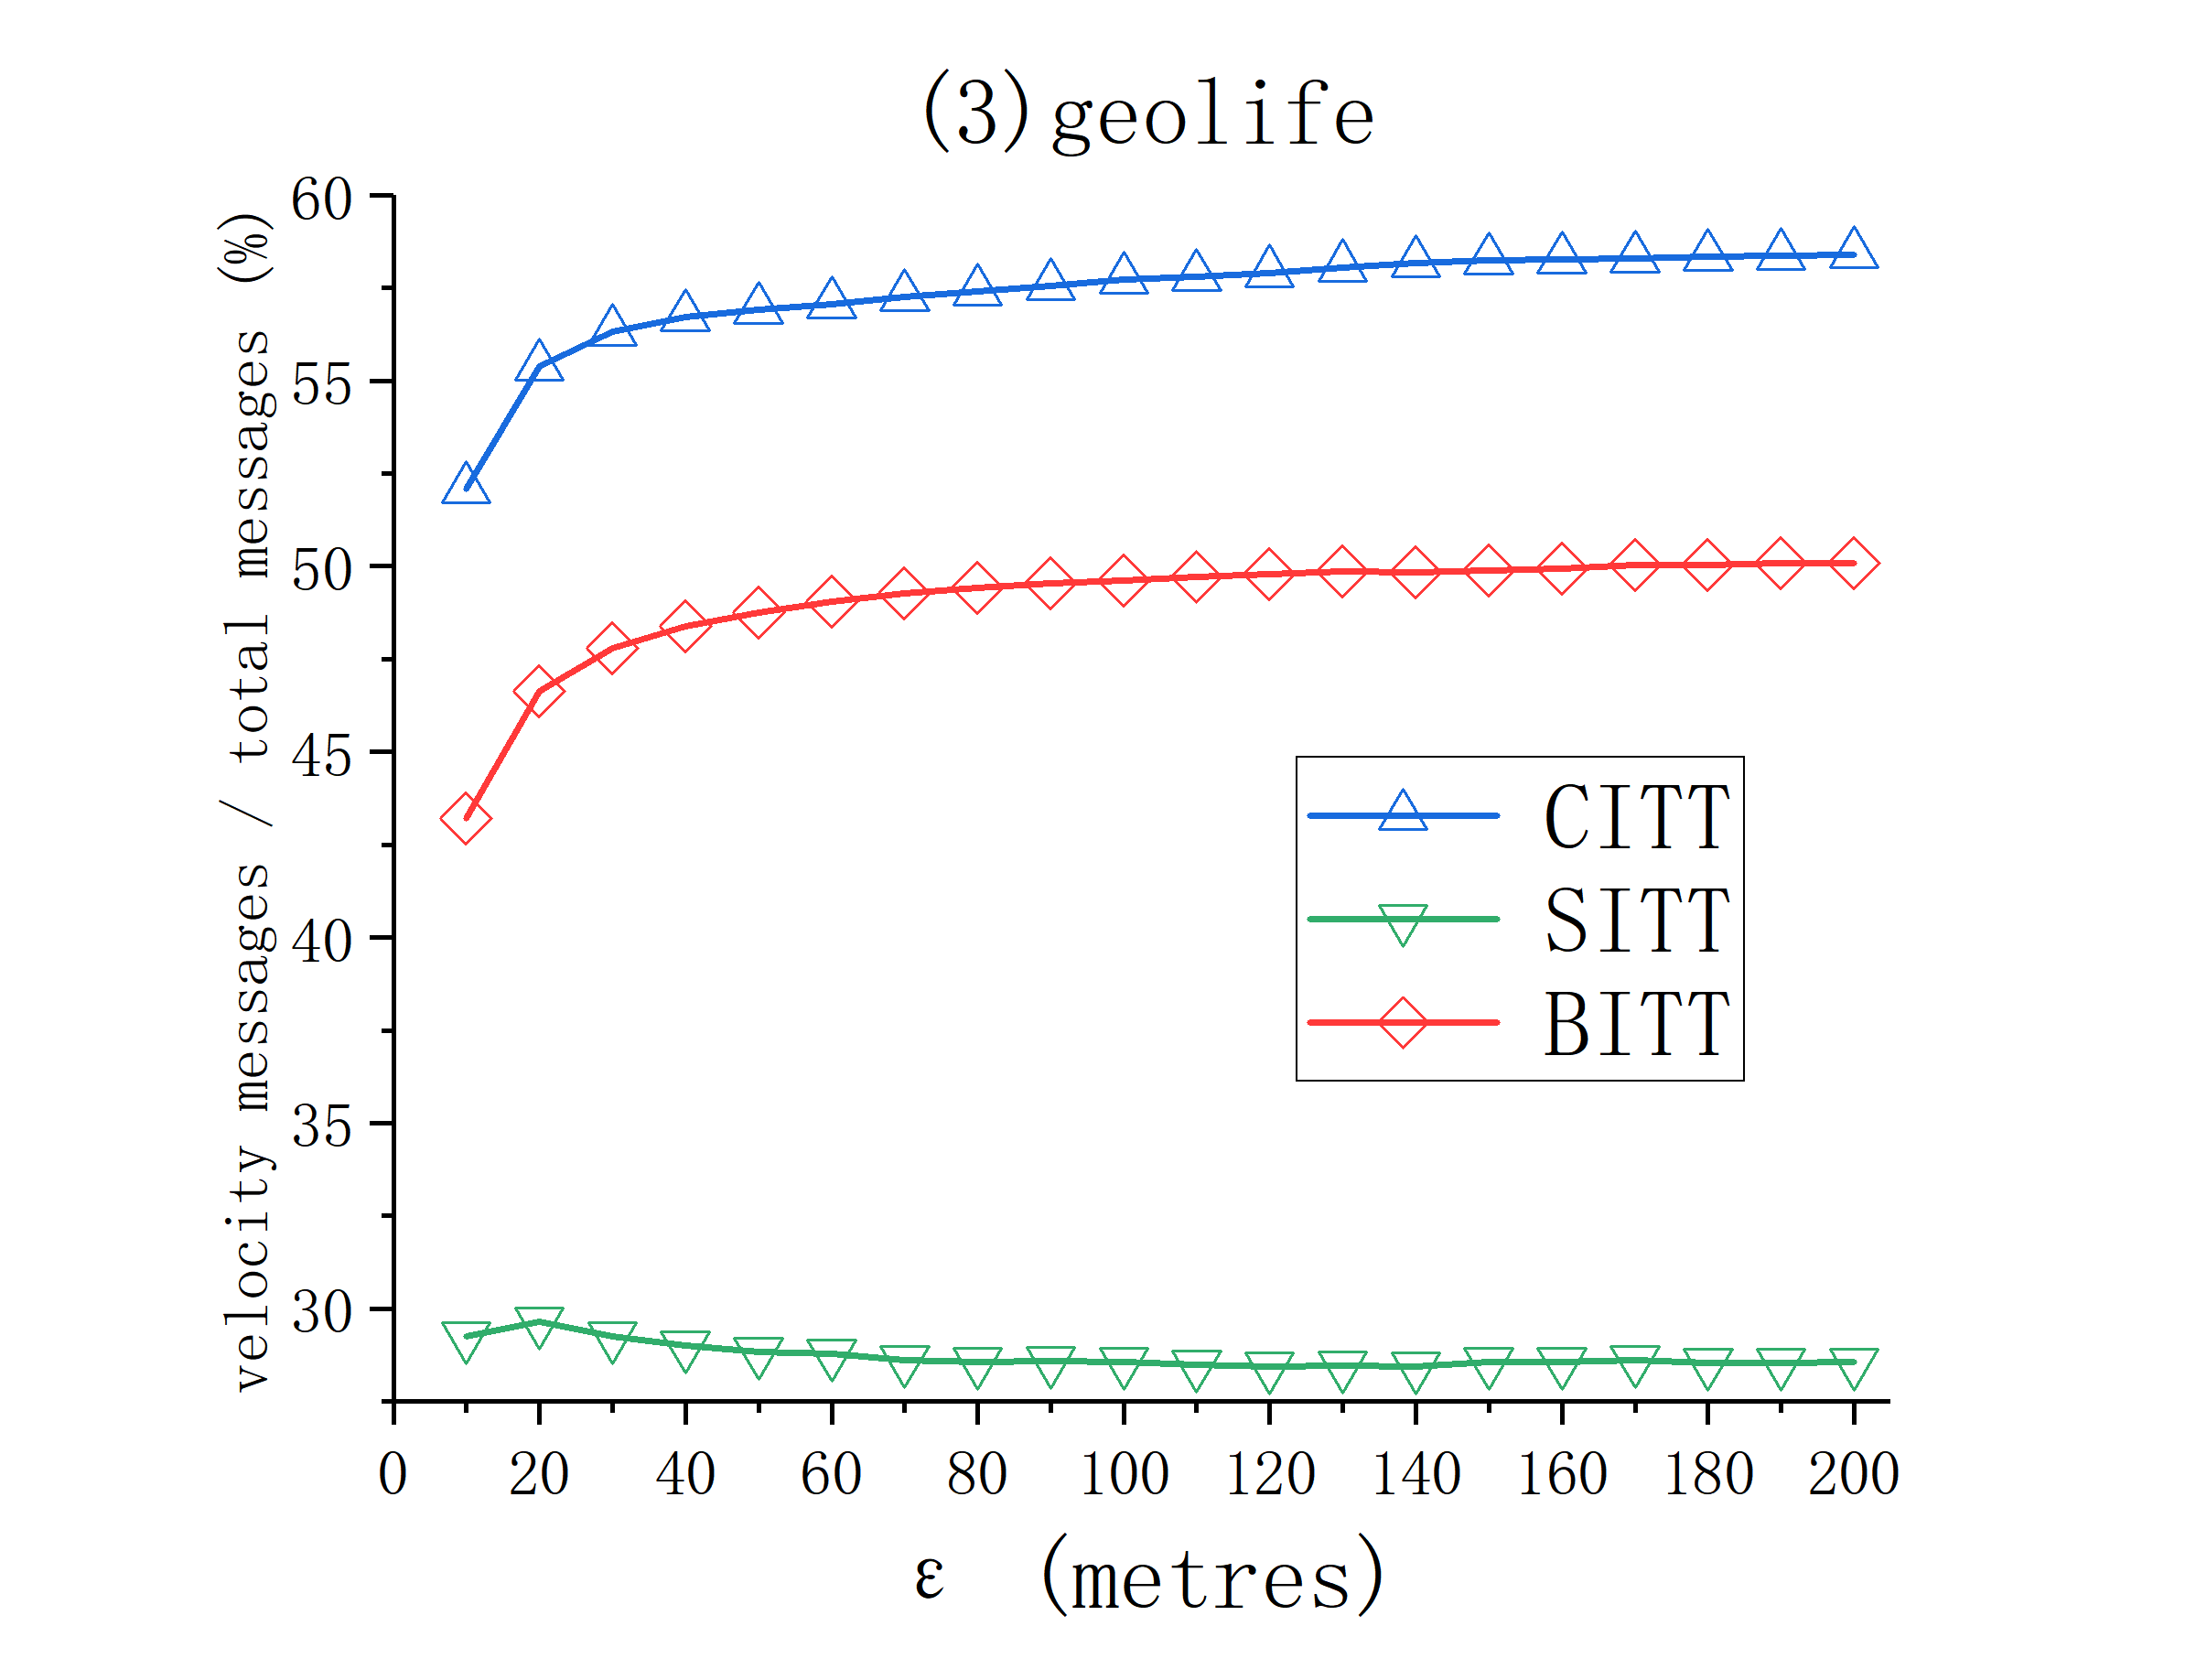
\includegraphics[scale = 0.210]{figures/Fig-geolife-speed-messages.png}\hspace{1ex}
	%\vspace{-1ex}
	\caption{\small Evaluation of velocities messages: varying error bounds $\epsilon_{sed}$ and $\epsilon_{ped}$.}
	\label{fig:speed-message}
	%\vspace{-1ex}
\end{figure*}

\stitle{Total messages.}
%To evaluate the impacts of distance metrics and error bounds on messages of \citt, \sitt and \bitt vs. \ldrh and \grts, we varied the error bound (either $\epsilon_{sed}$ or $\epsilon_{ped}$) from $10$ meters to $200$ meters on the entire three datasets, respectively. 

\ni (1) We can see that the amount of transmitted messages in the \ldrh is the largest, and this value is the smallest in \sitt, because the ped threshold is looser than sed.

\ni (2) Since \ldrh updates the position information every time the velocity is updated, the percentage of velocity updates has always been 50\%.

\ni (3) The proportions of velocities updates of \citt, \bitt, and \sitt are all greater than \ldrh, because these algorithms constantly calculate and update the velocity during the tracking process.

\ni (4) \grts has the least velocities update ratio. This is because \grts only updates the velocities messages when the buffer is cleared, and mainly transmits position information.



\begin{figure*}[tb!]
	\centering
	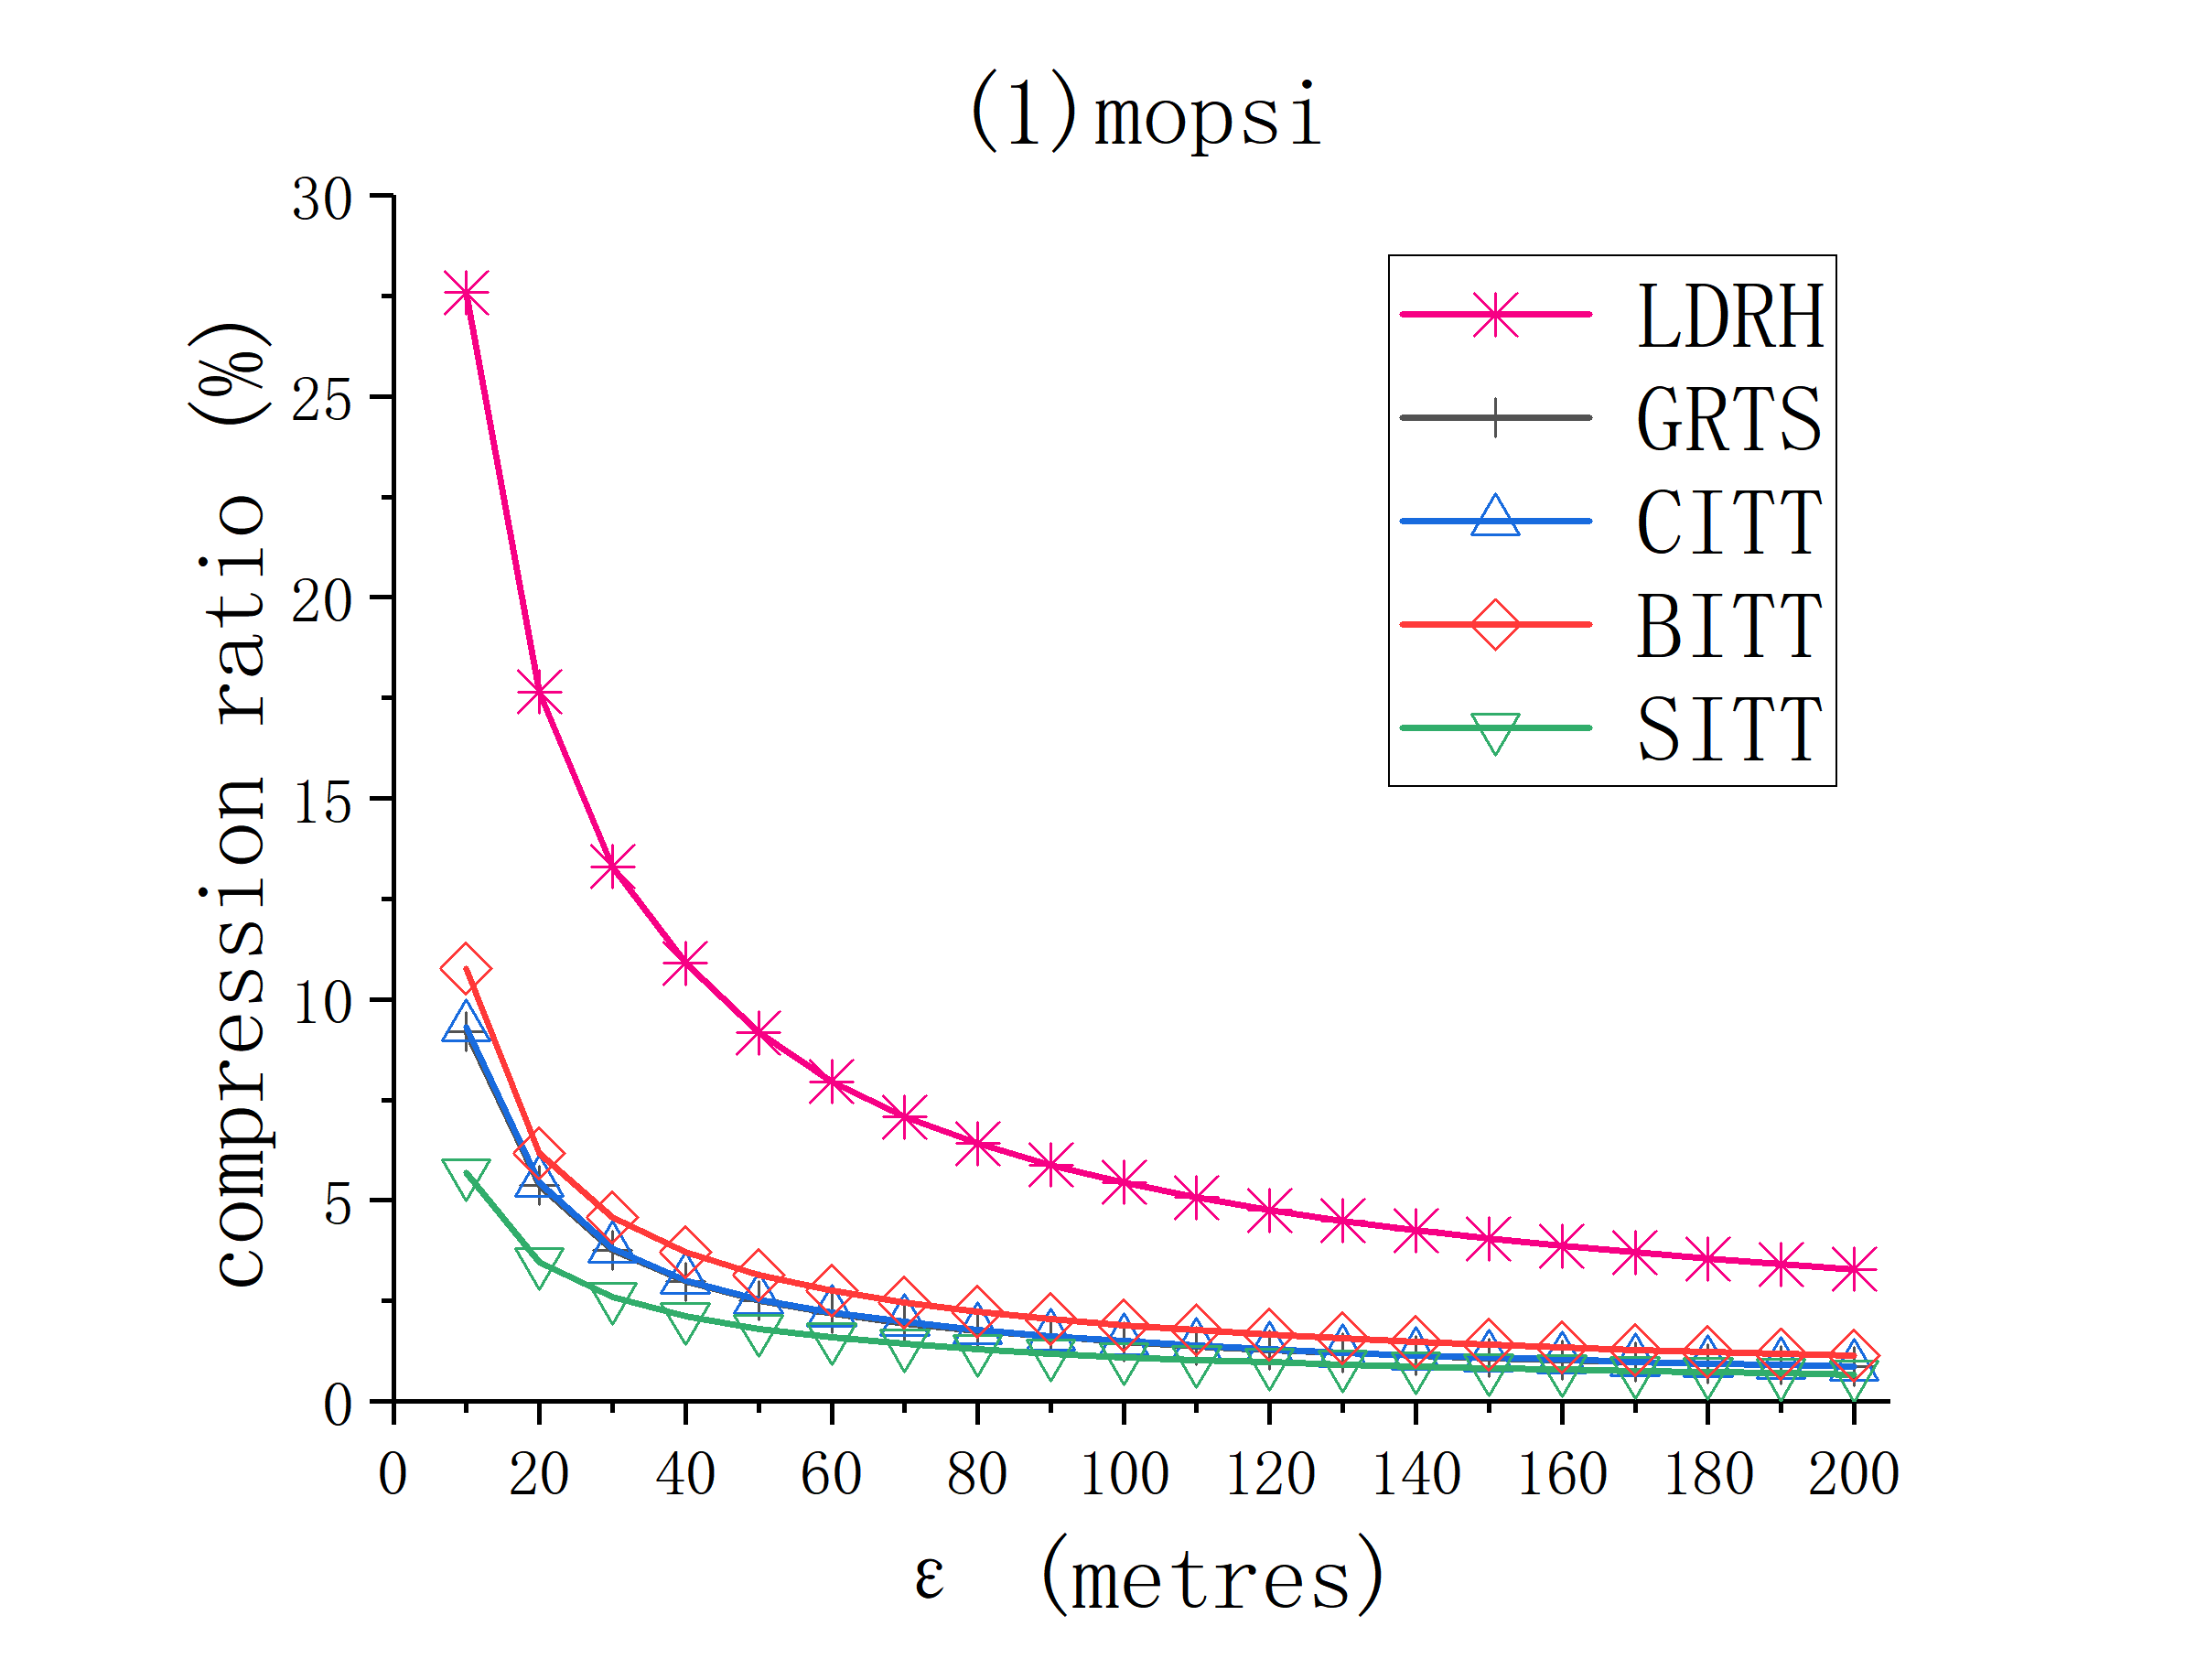
\includegraphics[scale = 0.210]{figures/Fig-mopsi-compression-ratio.png}\hspace{1ex}
	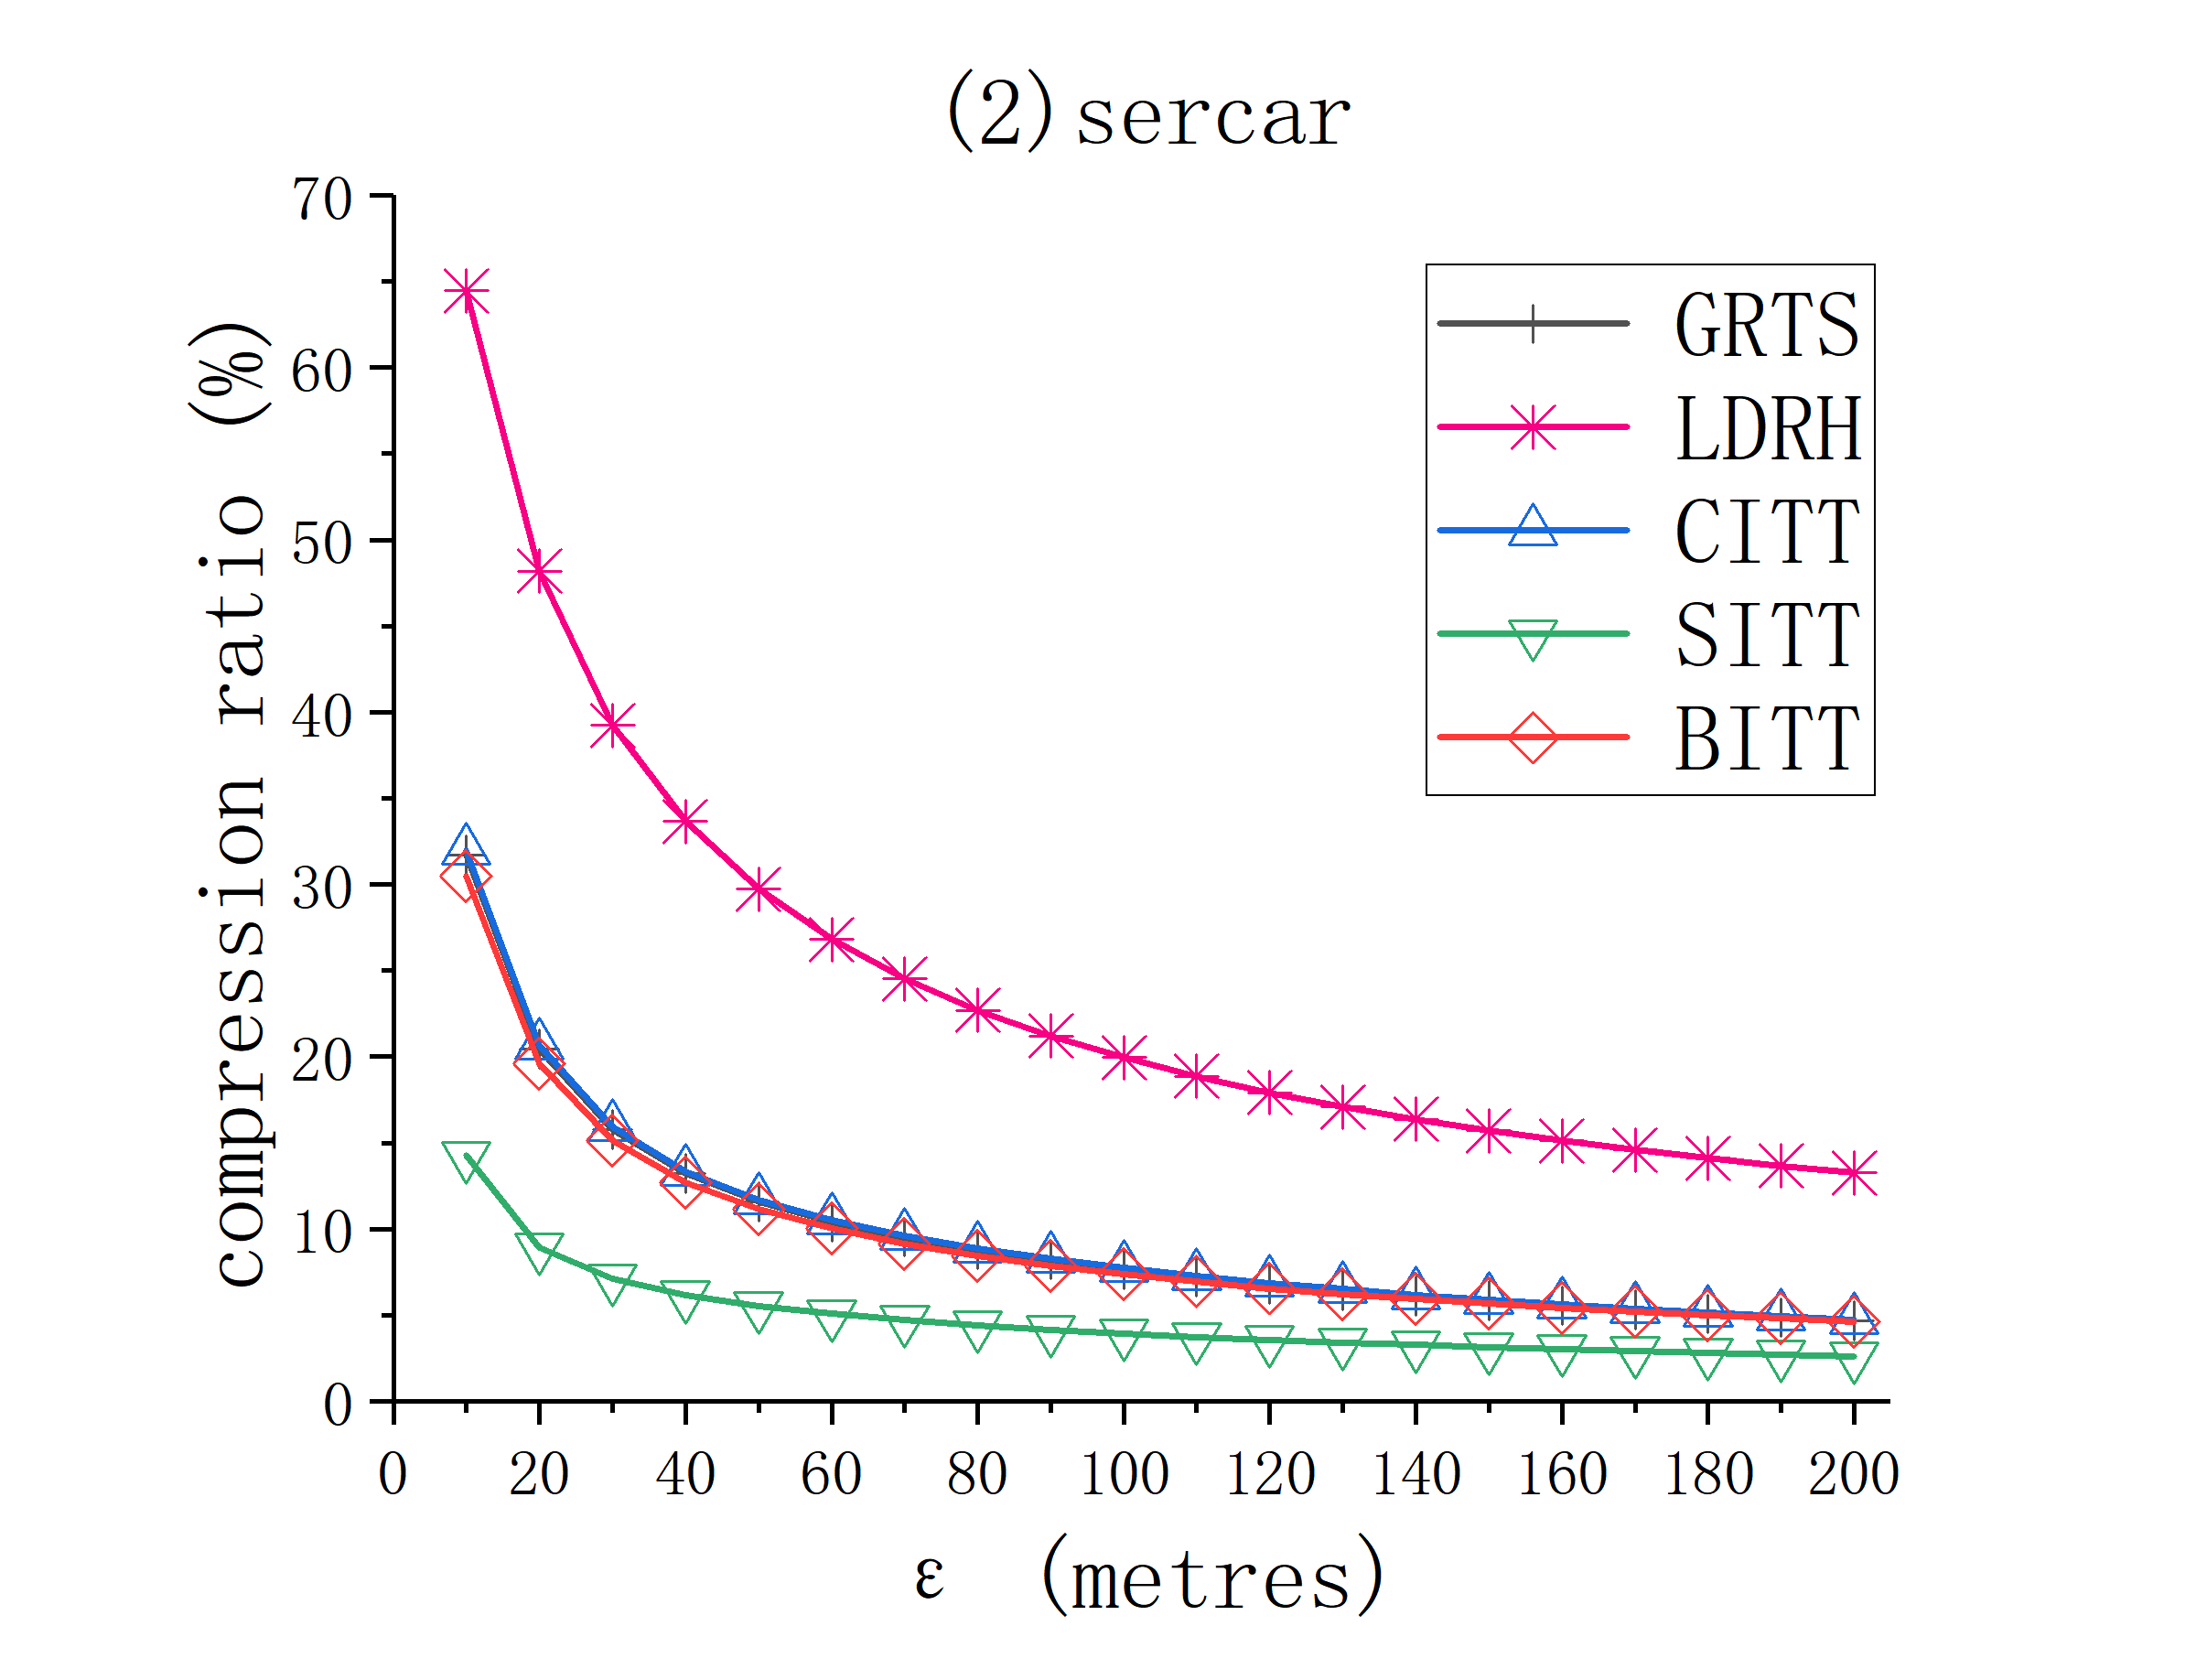
\includegraphics[scale = 0.210]{figures/Fig-sercar-compression-ratio.png}\hspace{1ex}
	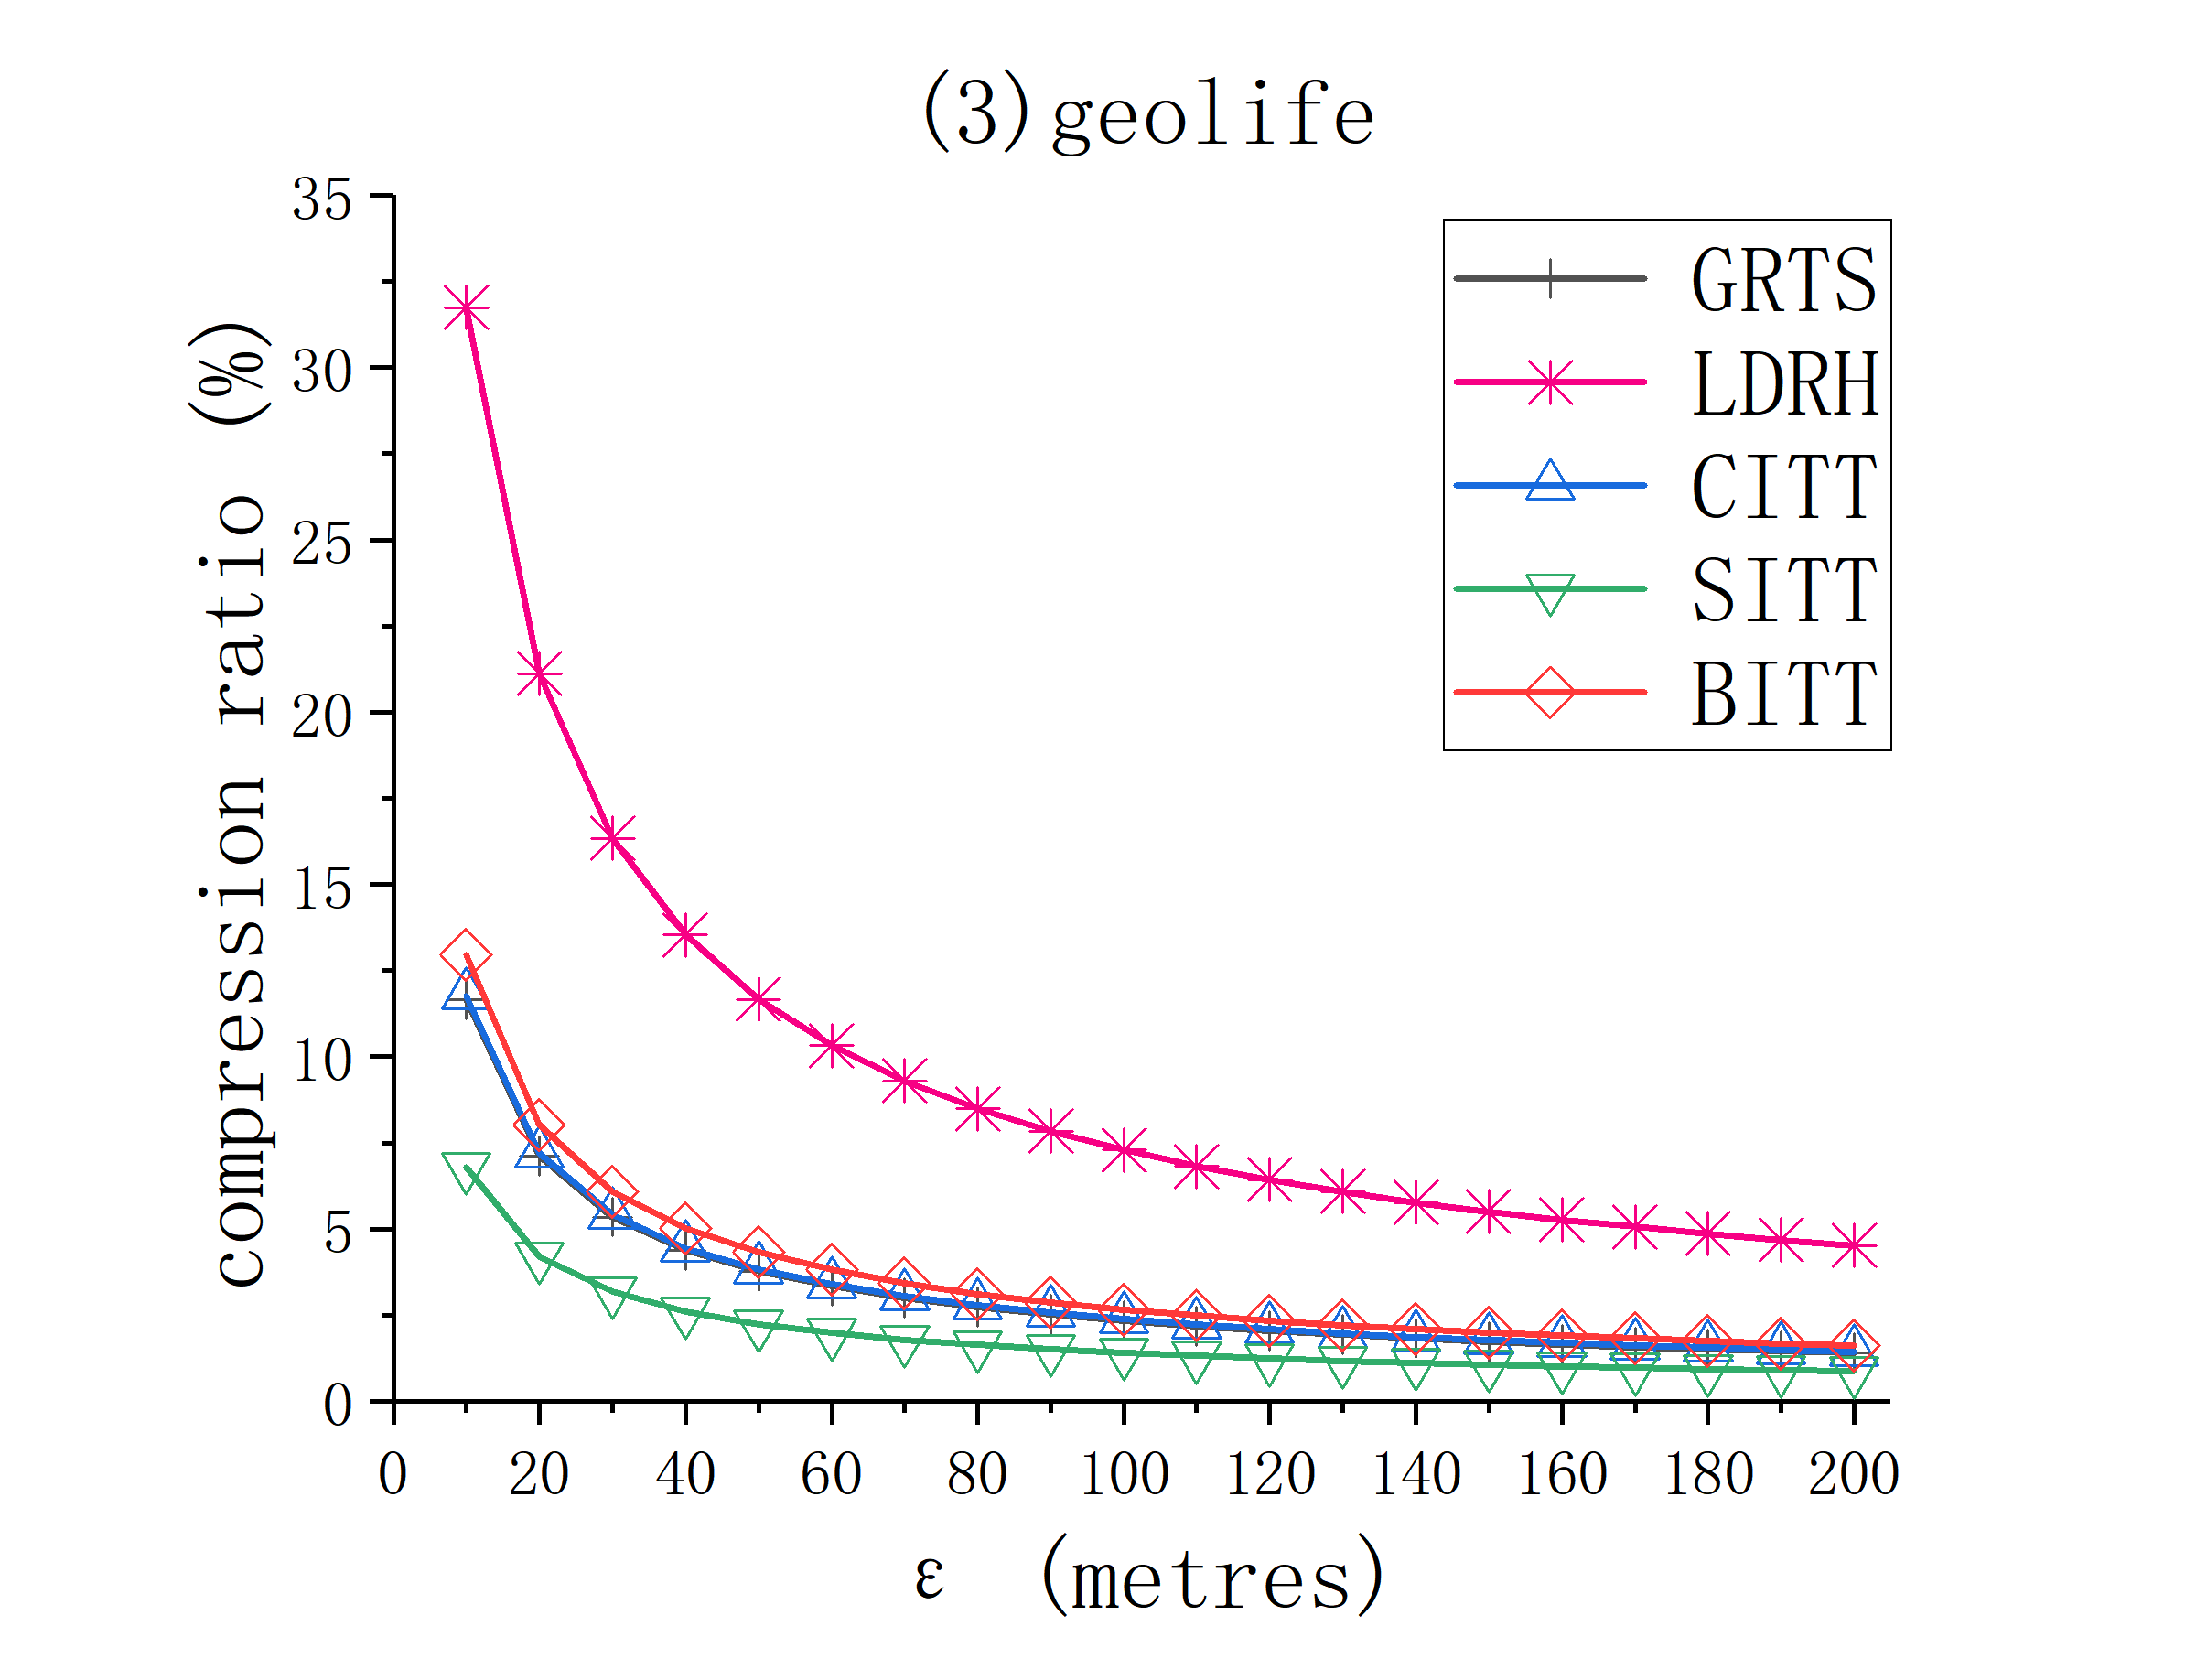
\includegraphics[scale = 0.210]{figures/Fig-geolife-compression-ratio.png}\hspace{1ex}
	%\vspace{-1ex}
	\caption{\small Evaluation of compression ratio: varying error bounds $\epsilon_{sed}$ and $\epsilon_{ped}$.}
	\label{fig:compression-ratio}
	%\vspace{-1ex}
\end{figure*}


\stitle{Compression ratios.}
\ni (1) When increasing $\epsilon_{sed}$ and $\epsilon_{ped}$, the compression ratios of all these algorithms decrease on all datasets.

\ni (2) Algorithm \citt is better than \ldrh {and comparable} with \grts on all datasets and for all $\epsilon$.
The compression ratios of \citt are on average {($29.0\%$, $40.4\%$, $33.5\%$) and ($101.0\%$, $100.9\%$, $101.6\%$)} of \ldrh and
\grts on {datasets (\mopsi, \sercar, \geolife)}, respectively.
For example, when $\epsilon$ = $40$ meters, the compression ratios of algorithms
\ldrh, \citt and \grts are
{($10.9\%$, $33.7\%$, $13.6\%$), ($3.0\%$, $13.3\%$, $4.5\%$) and ($3.0\%$, $13.2\%$, $4.4\%$)} on  {datasets (\mopsi, \sercar, \geolife)}, respectively.

\ni (3) Algorithm \sitt has better compression ratios than \ldrh, \citt and \grts on all datasets and for all $\epsilon$.
The compression ratios of \sitt are on average ($20.0\%$, $69.2\%$, $69.9\%$), ($19.6\%$, $48.4\%$, $48.9\%$) and {($19.7\%$, $58.7\%$, $59.6\%$) of algorithms
	\ldrh, \citt and \grts on {datasets (\mopsi, \sercar, \geolife)}, respectively.
	For example, when $\epsilon$ = $40$ meters, the compression ratios of algorithm
	\sitt are ($2.1\%$, $6.1\%$, $2.6\%$) on datasets (\mopsi, \sercar, \geolife), respectively.
	
	\ni (4) The compression ratios of algorithm \bitt are between \citt and \sitt.







\begin{figure*}[tb!]
	\centering
	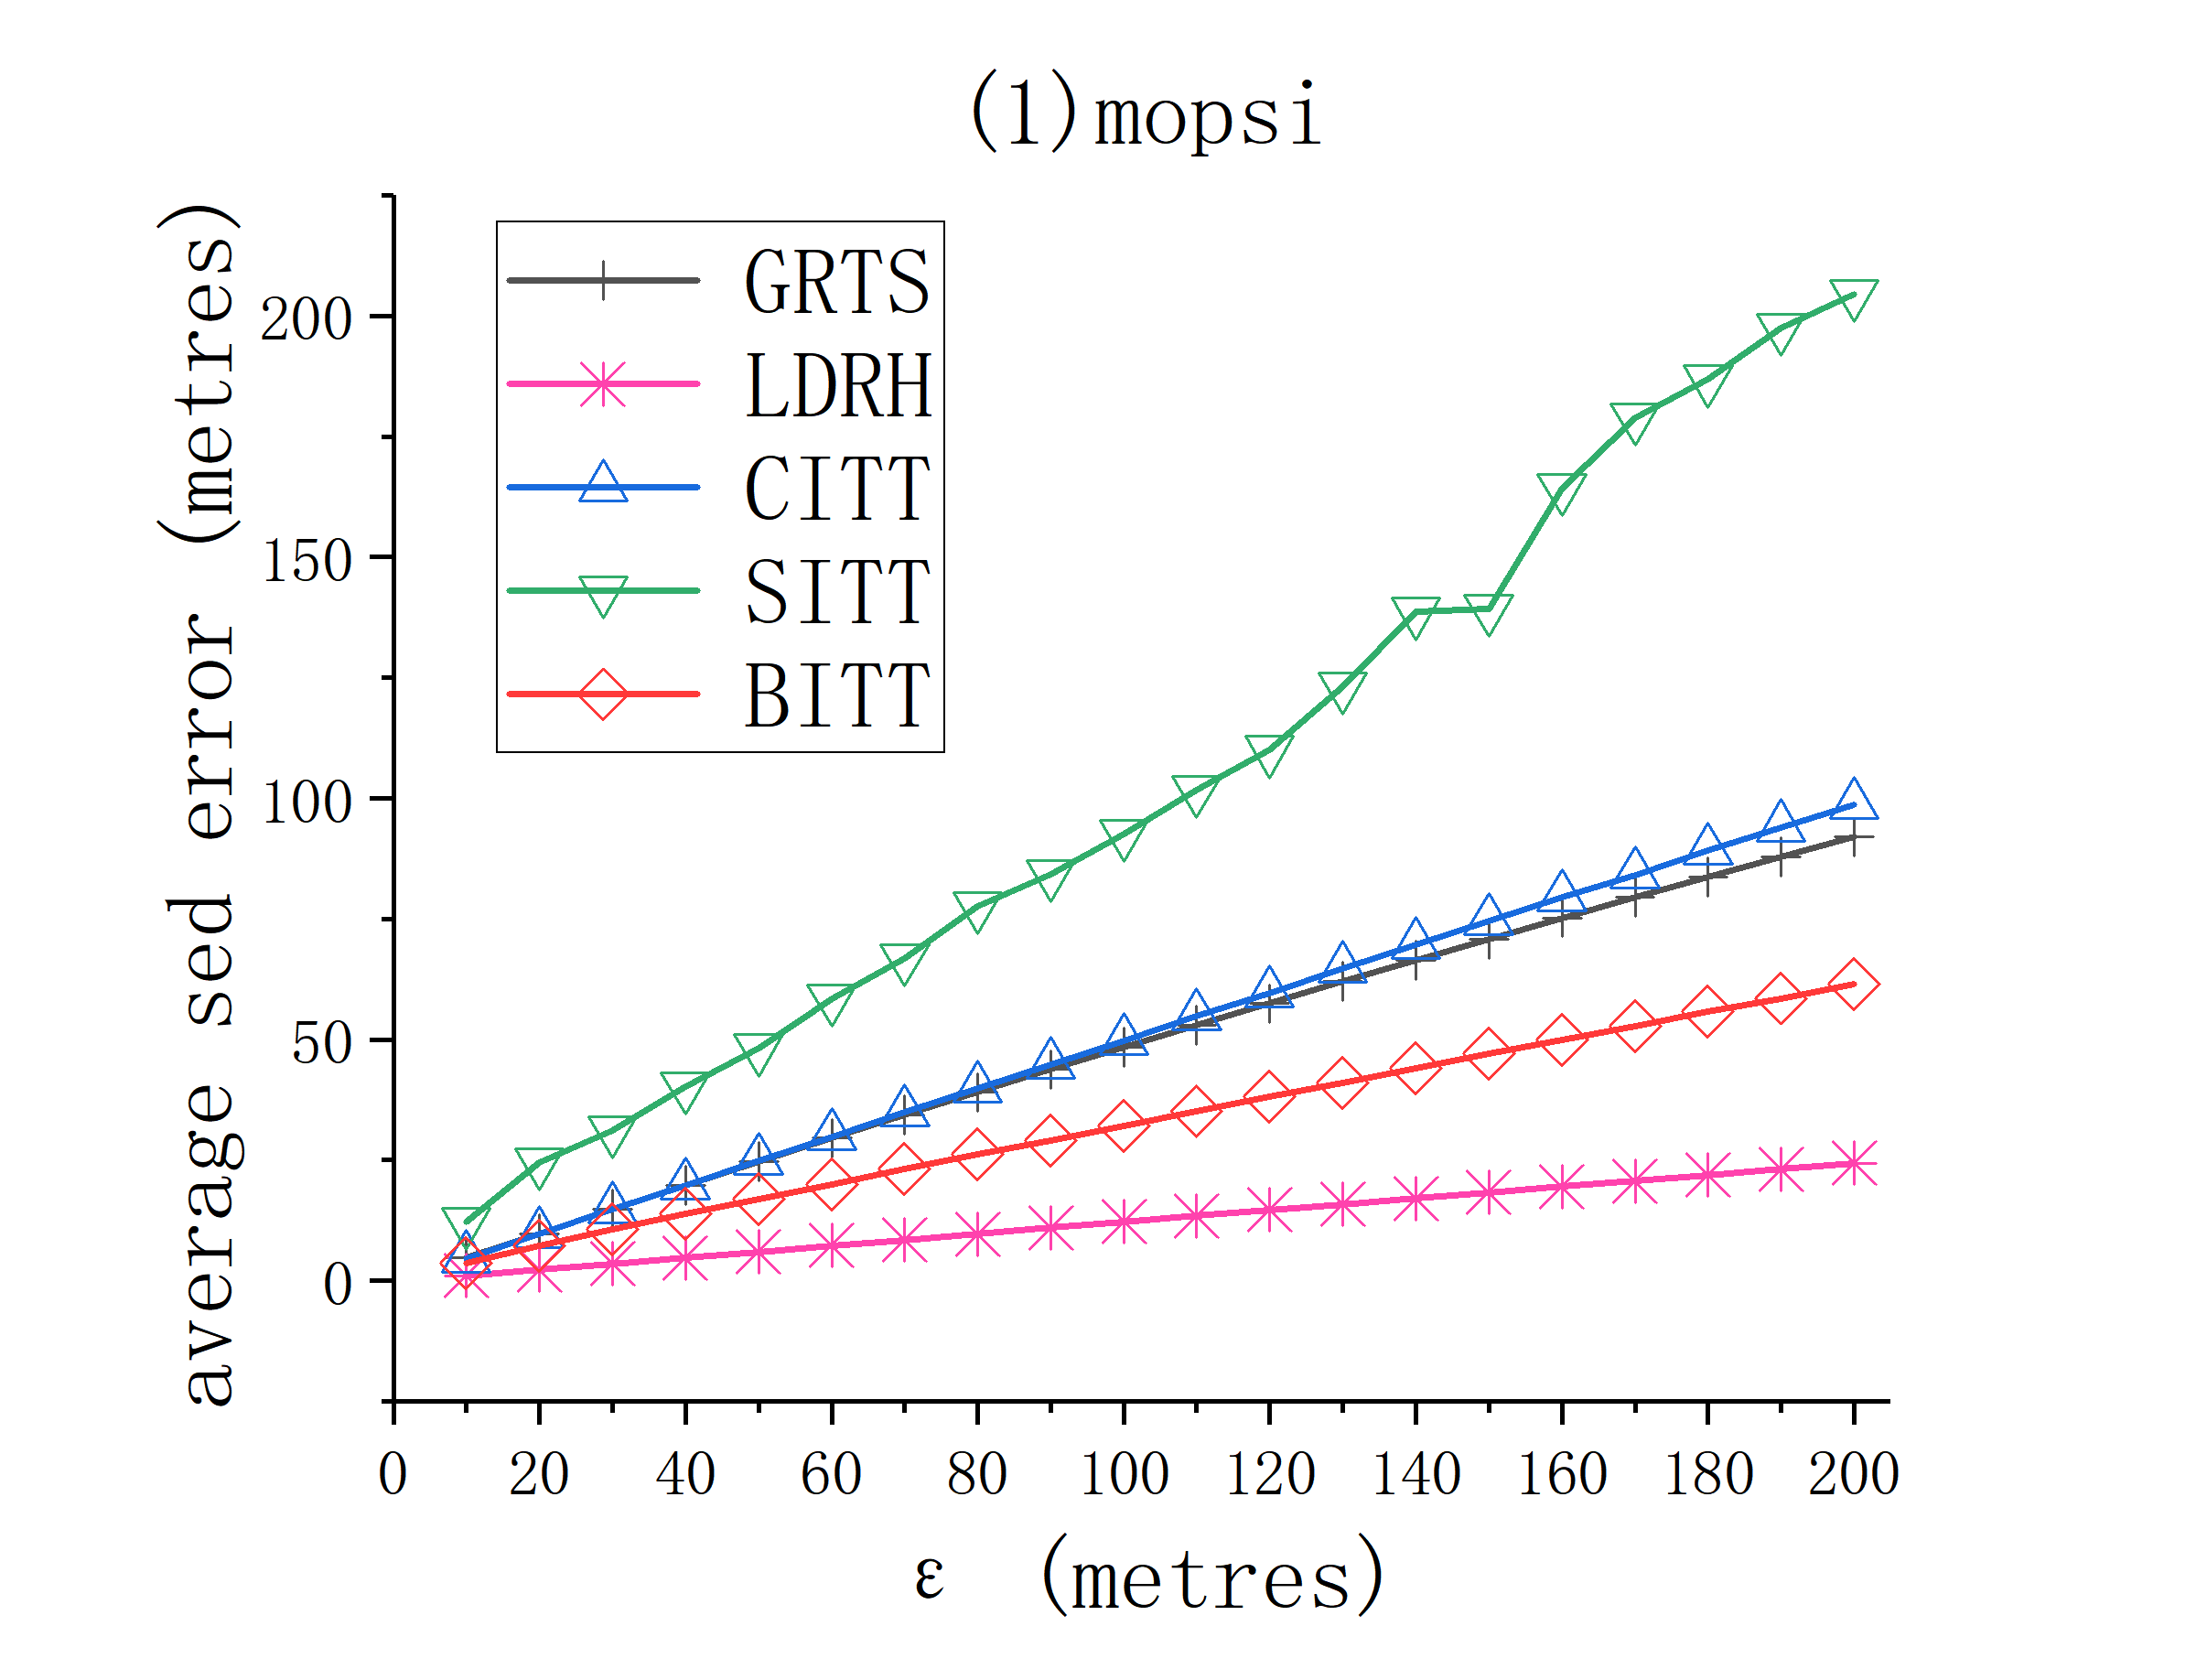
\includegraphics[scale = 0.210]{figures/Fig-mopsi-sed-error.png}\hspace{1ex}
	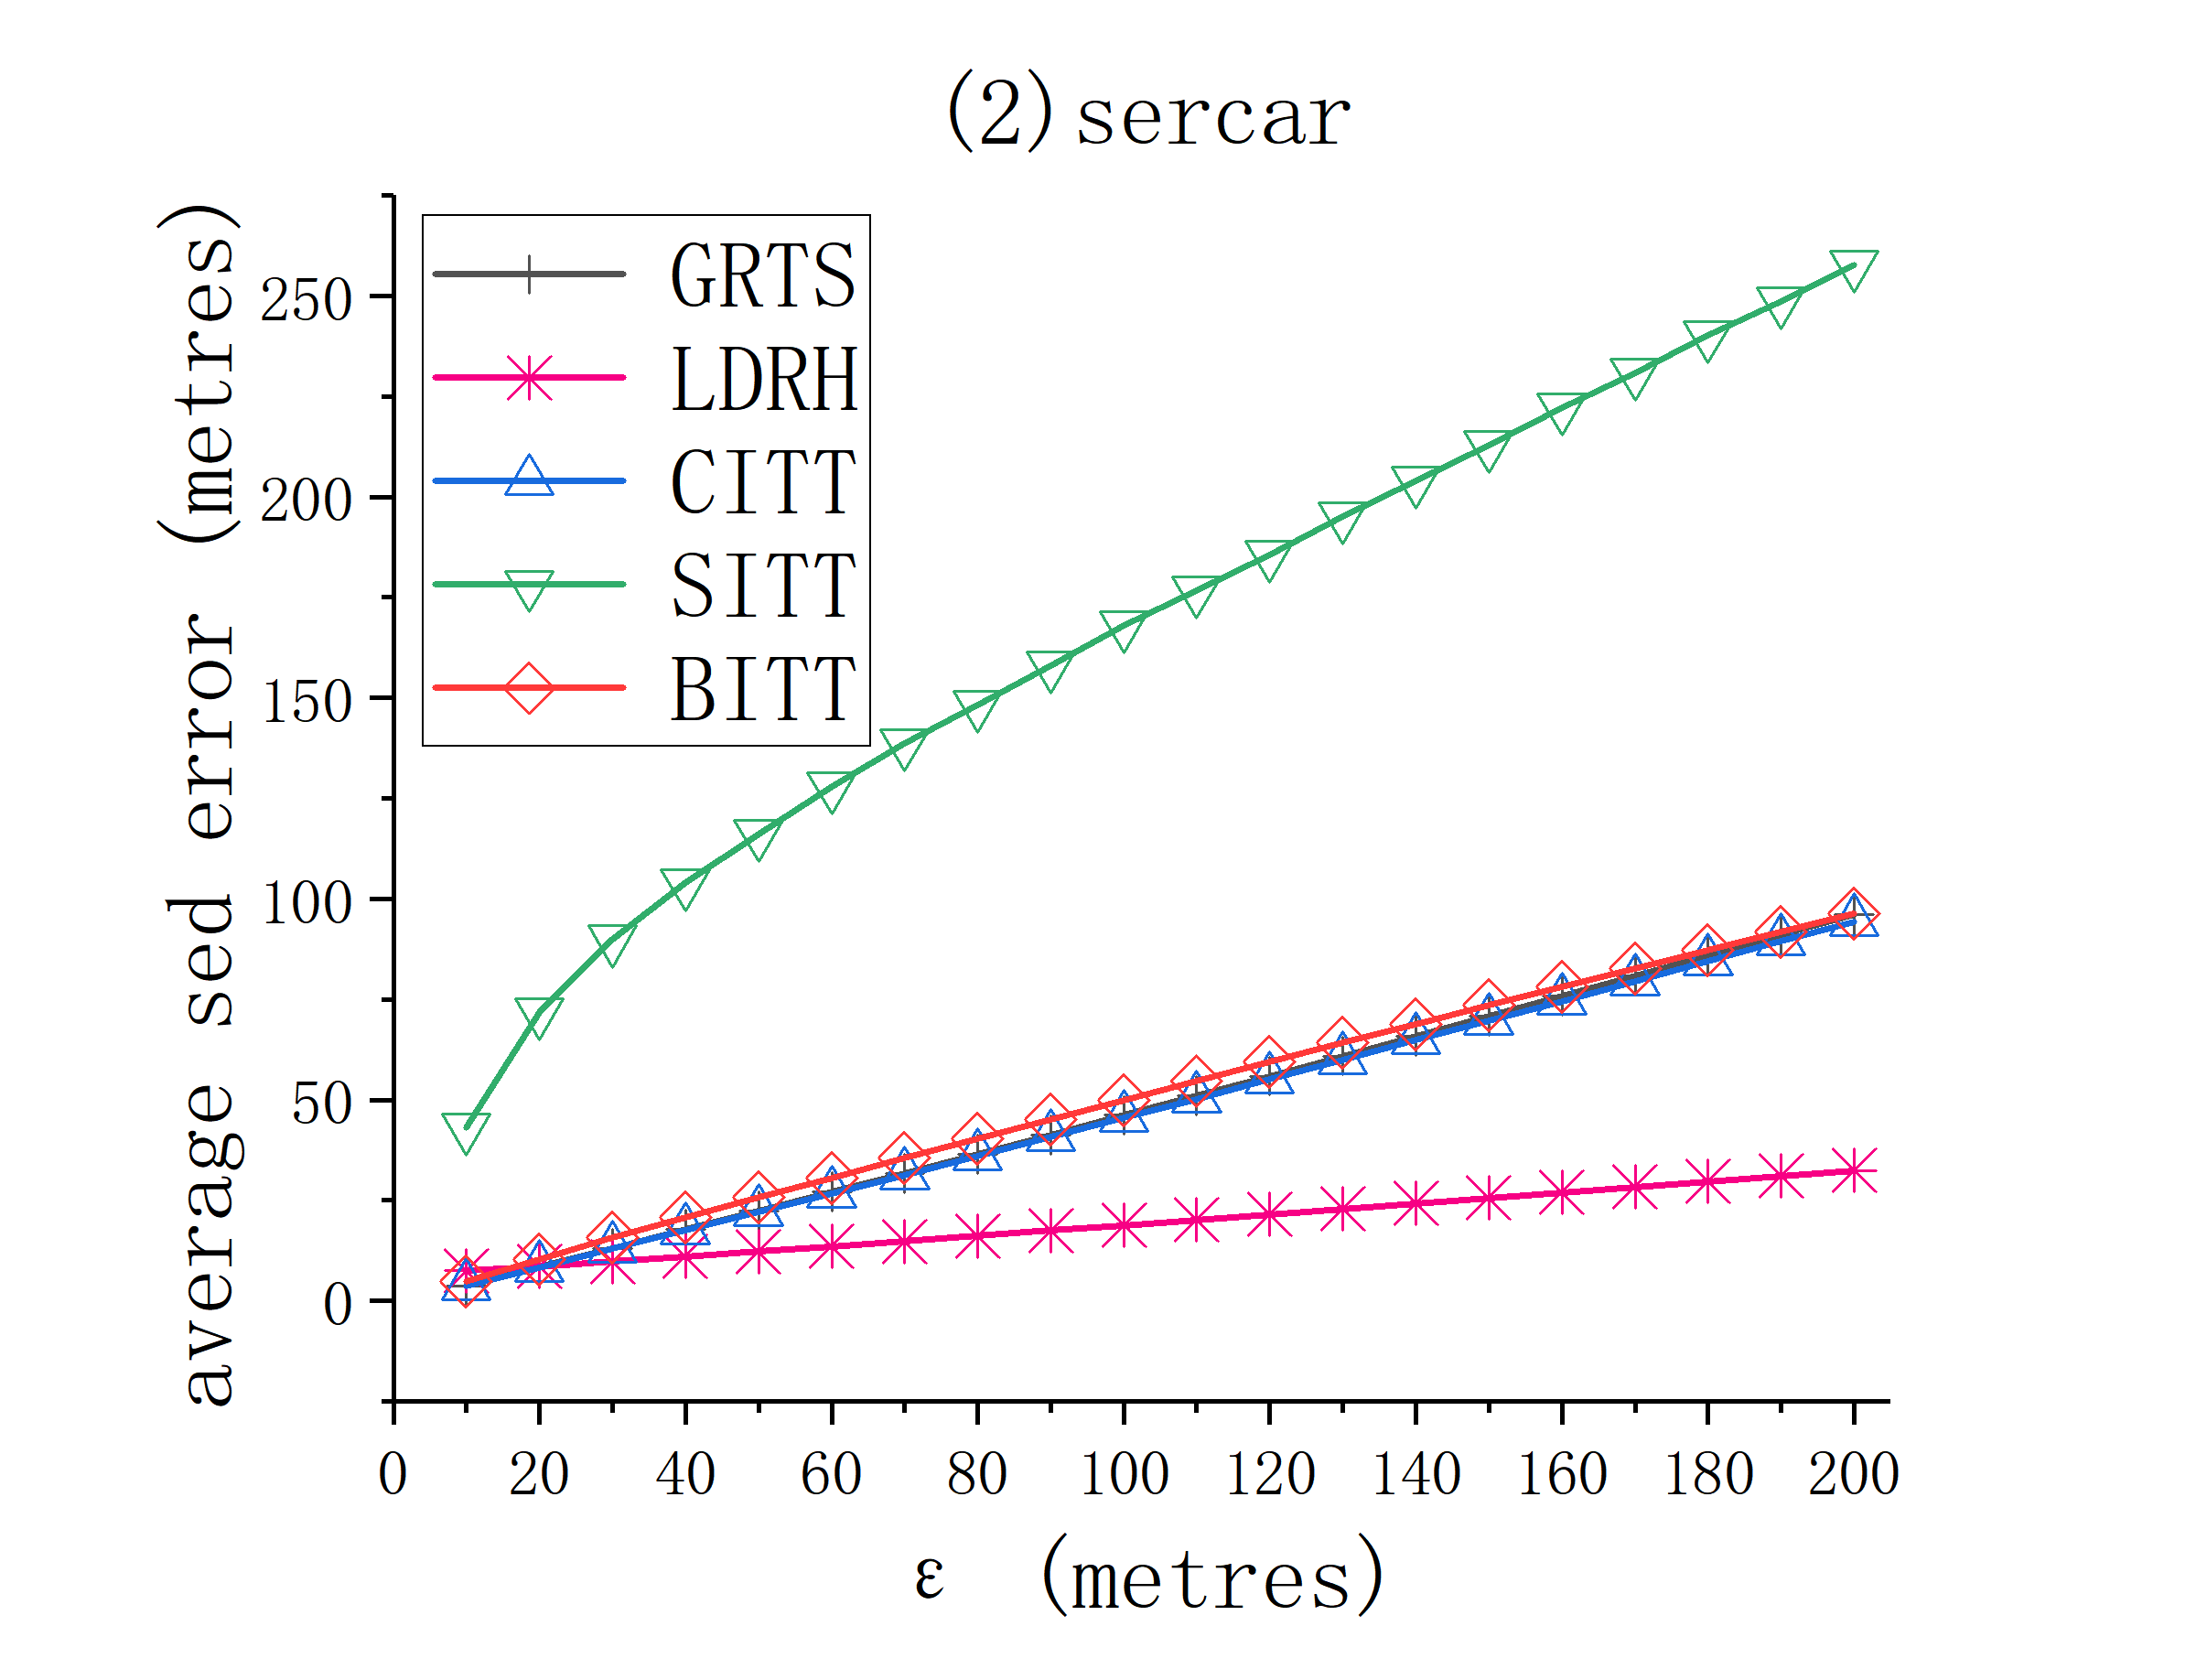
\includegraphics[scale = 0.210]{figures/Fig-sercar-sed-error.png}\hspace{1ex}
	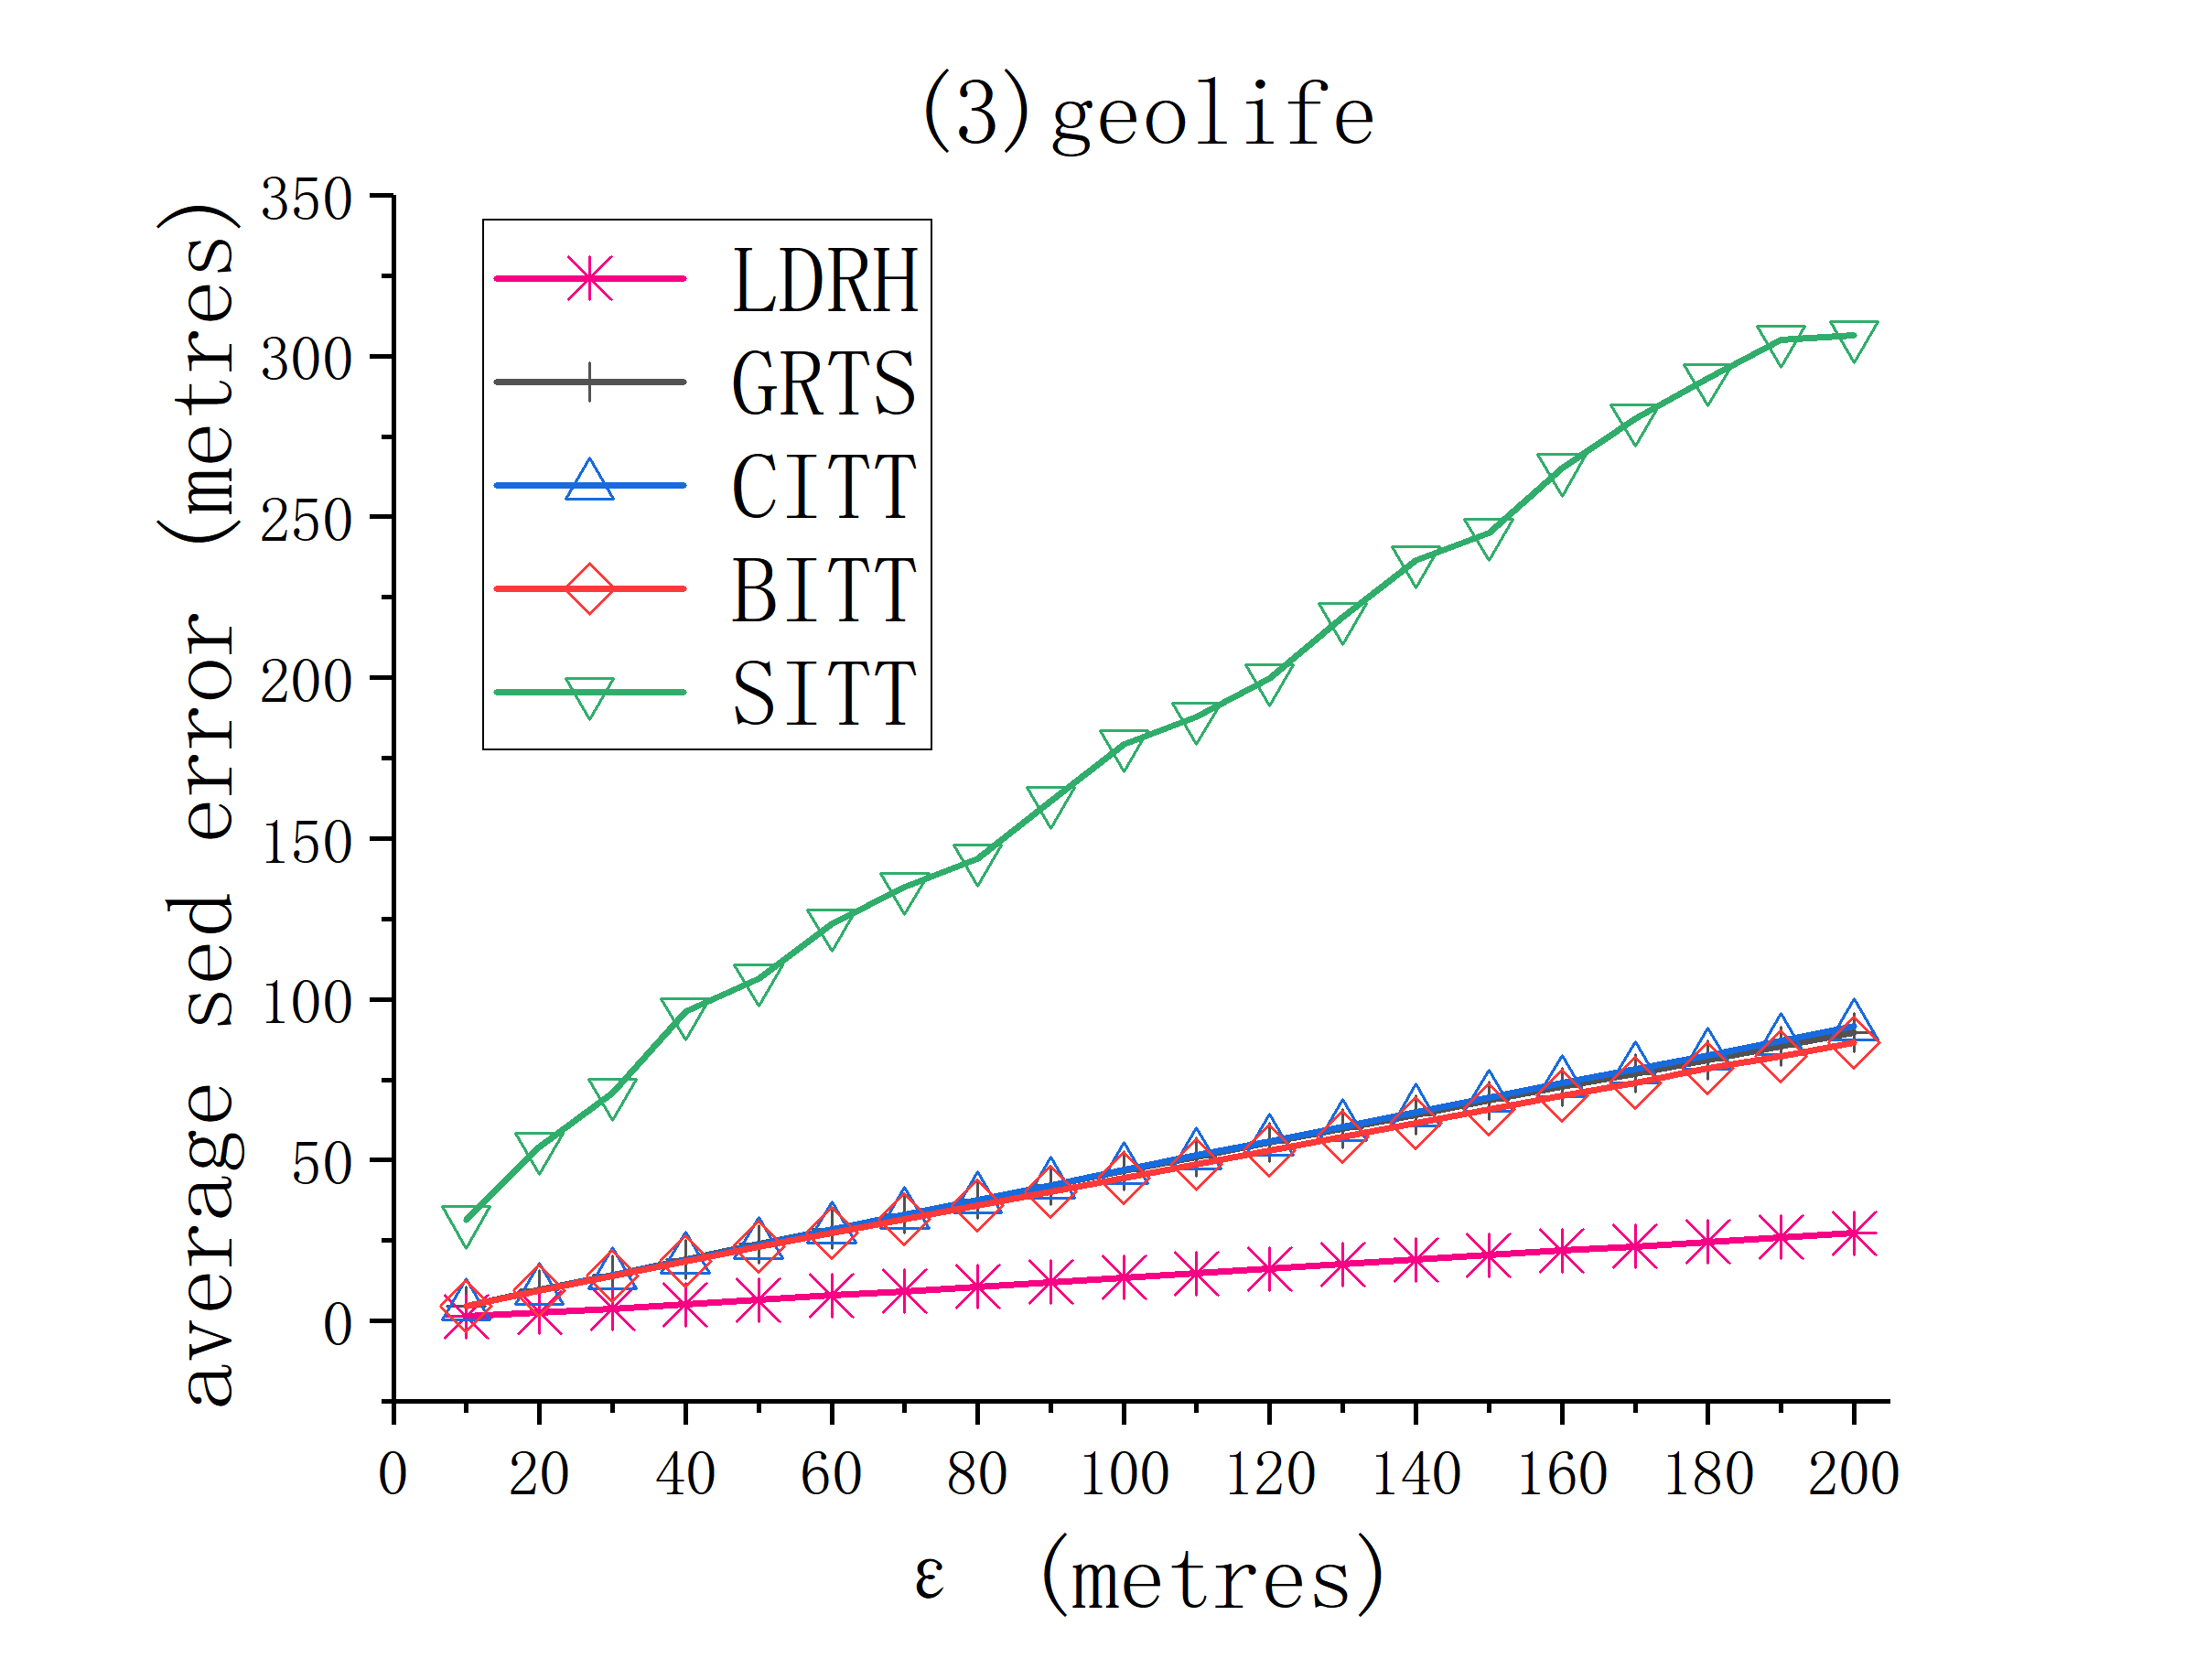
\includegraphics[scale = 0.210]{figures/Fig-geolife-sed-error.png}\hspace{1ex}
	%\vspace{-1ex}
	\caption{\small Evaluation of sed error: varying error bounds $\epsilon_{sed}$ and $\epsilon_{ped}$.}
	\label{fig:sed-error}
	%\vspace{-1ex}
\end{figure*}

\begin{figure*}[tb!]
	\centering
	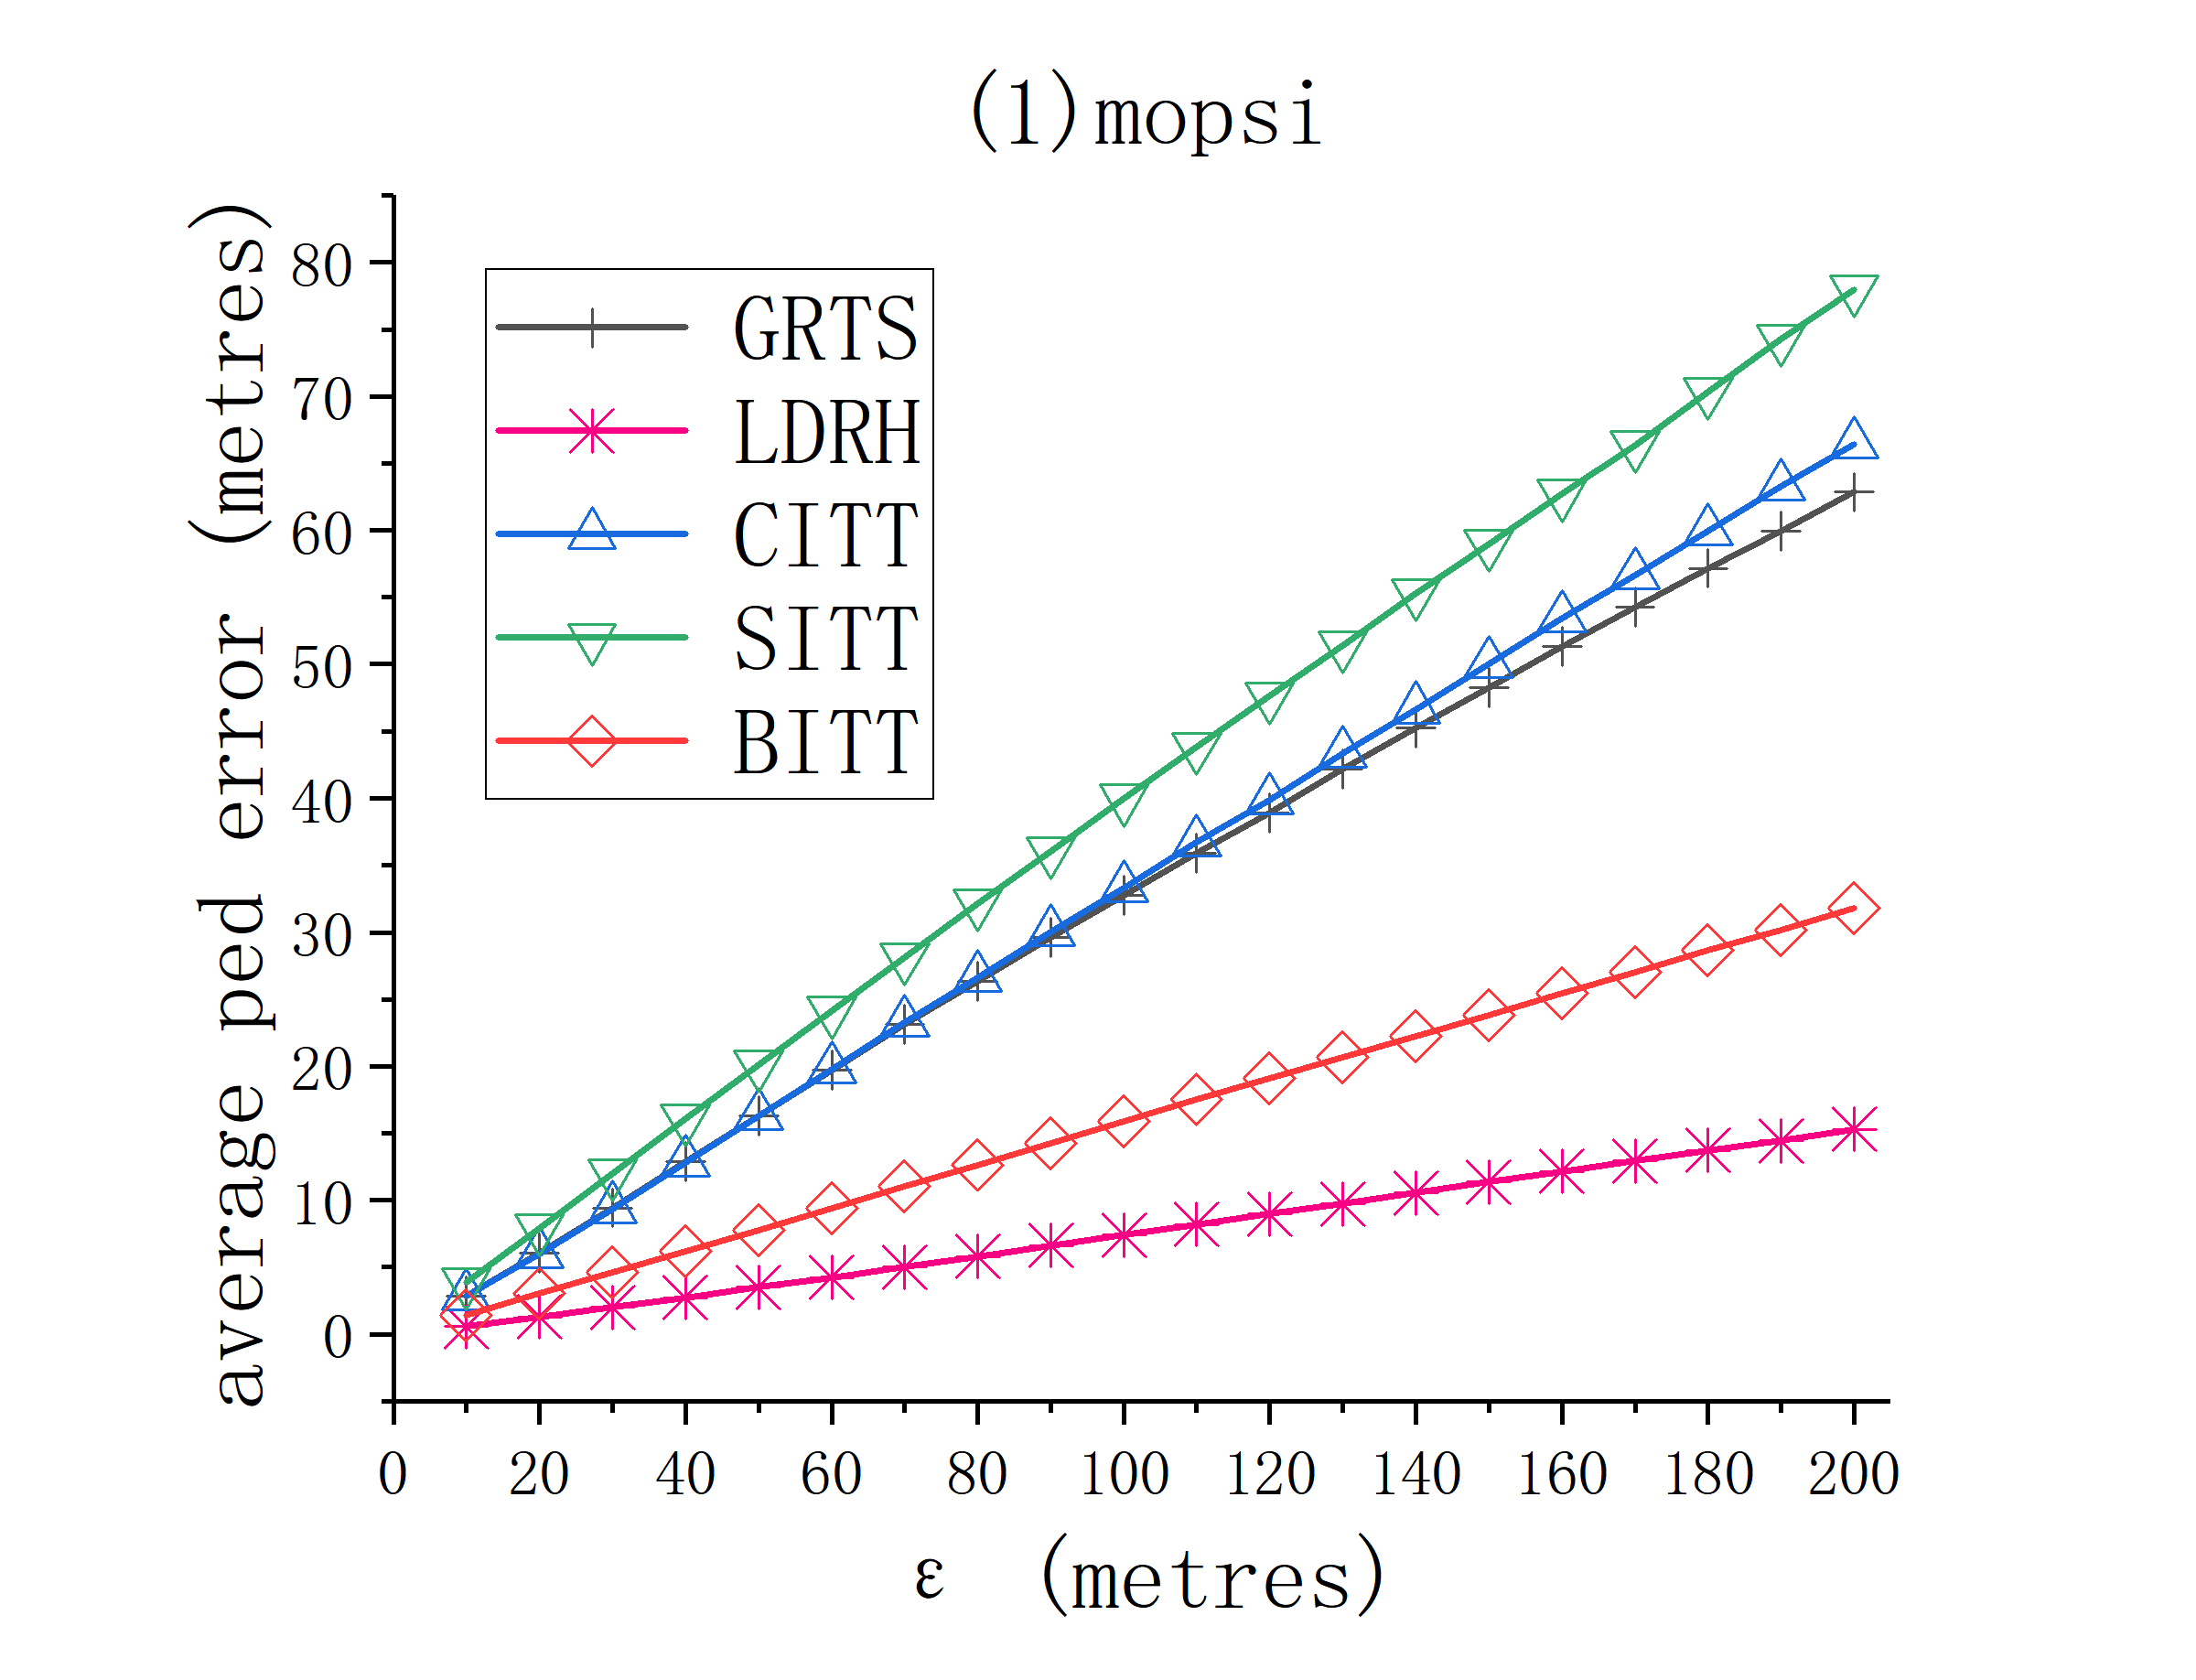
\includegraphics[scale = 0.210]{figures/Fig-mopsi-ped-error.png}\hspace{1ex}
	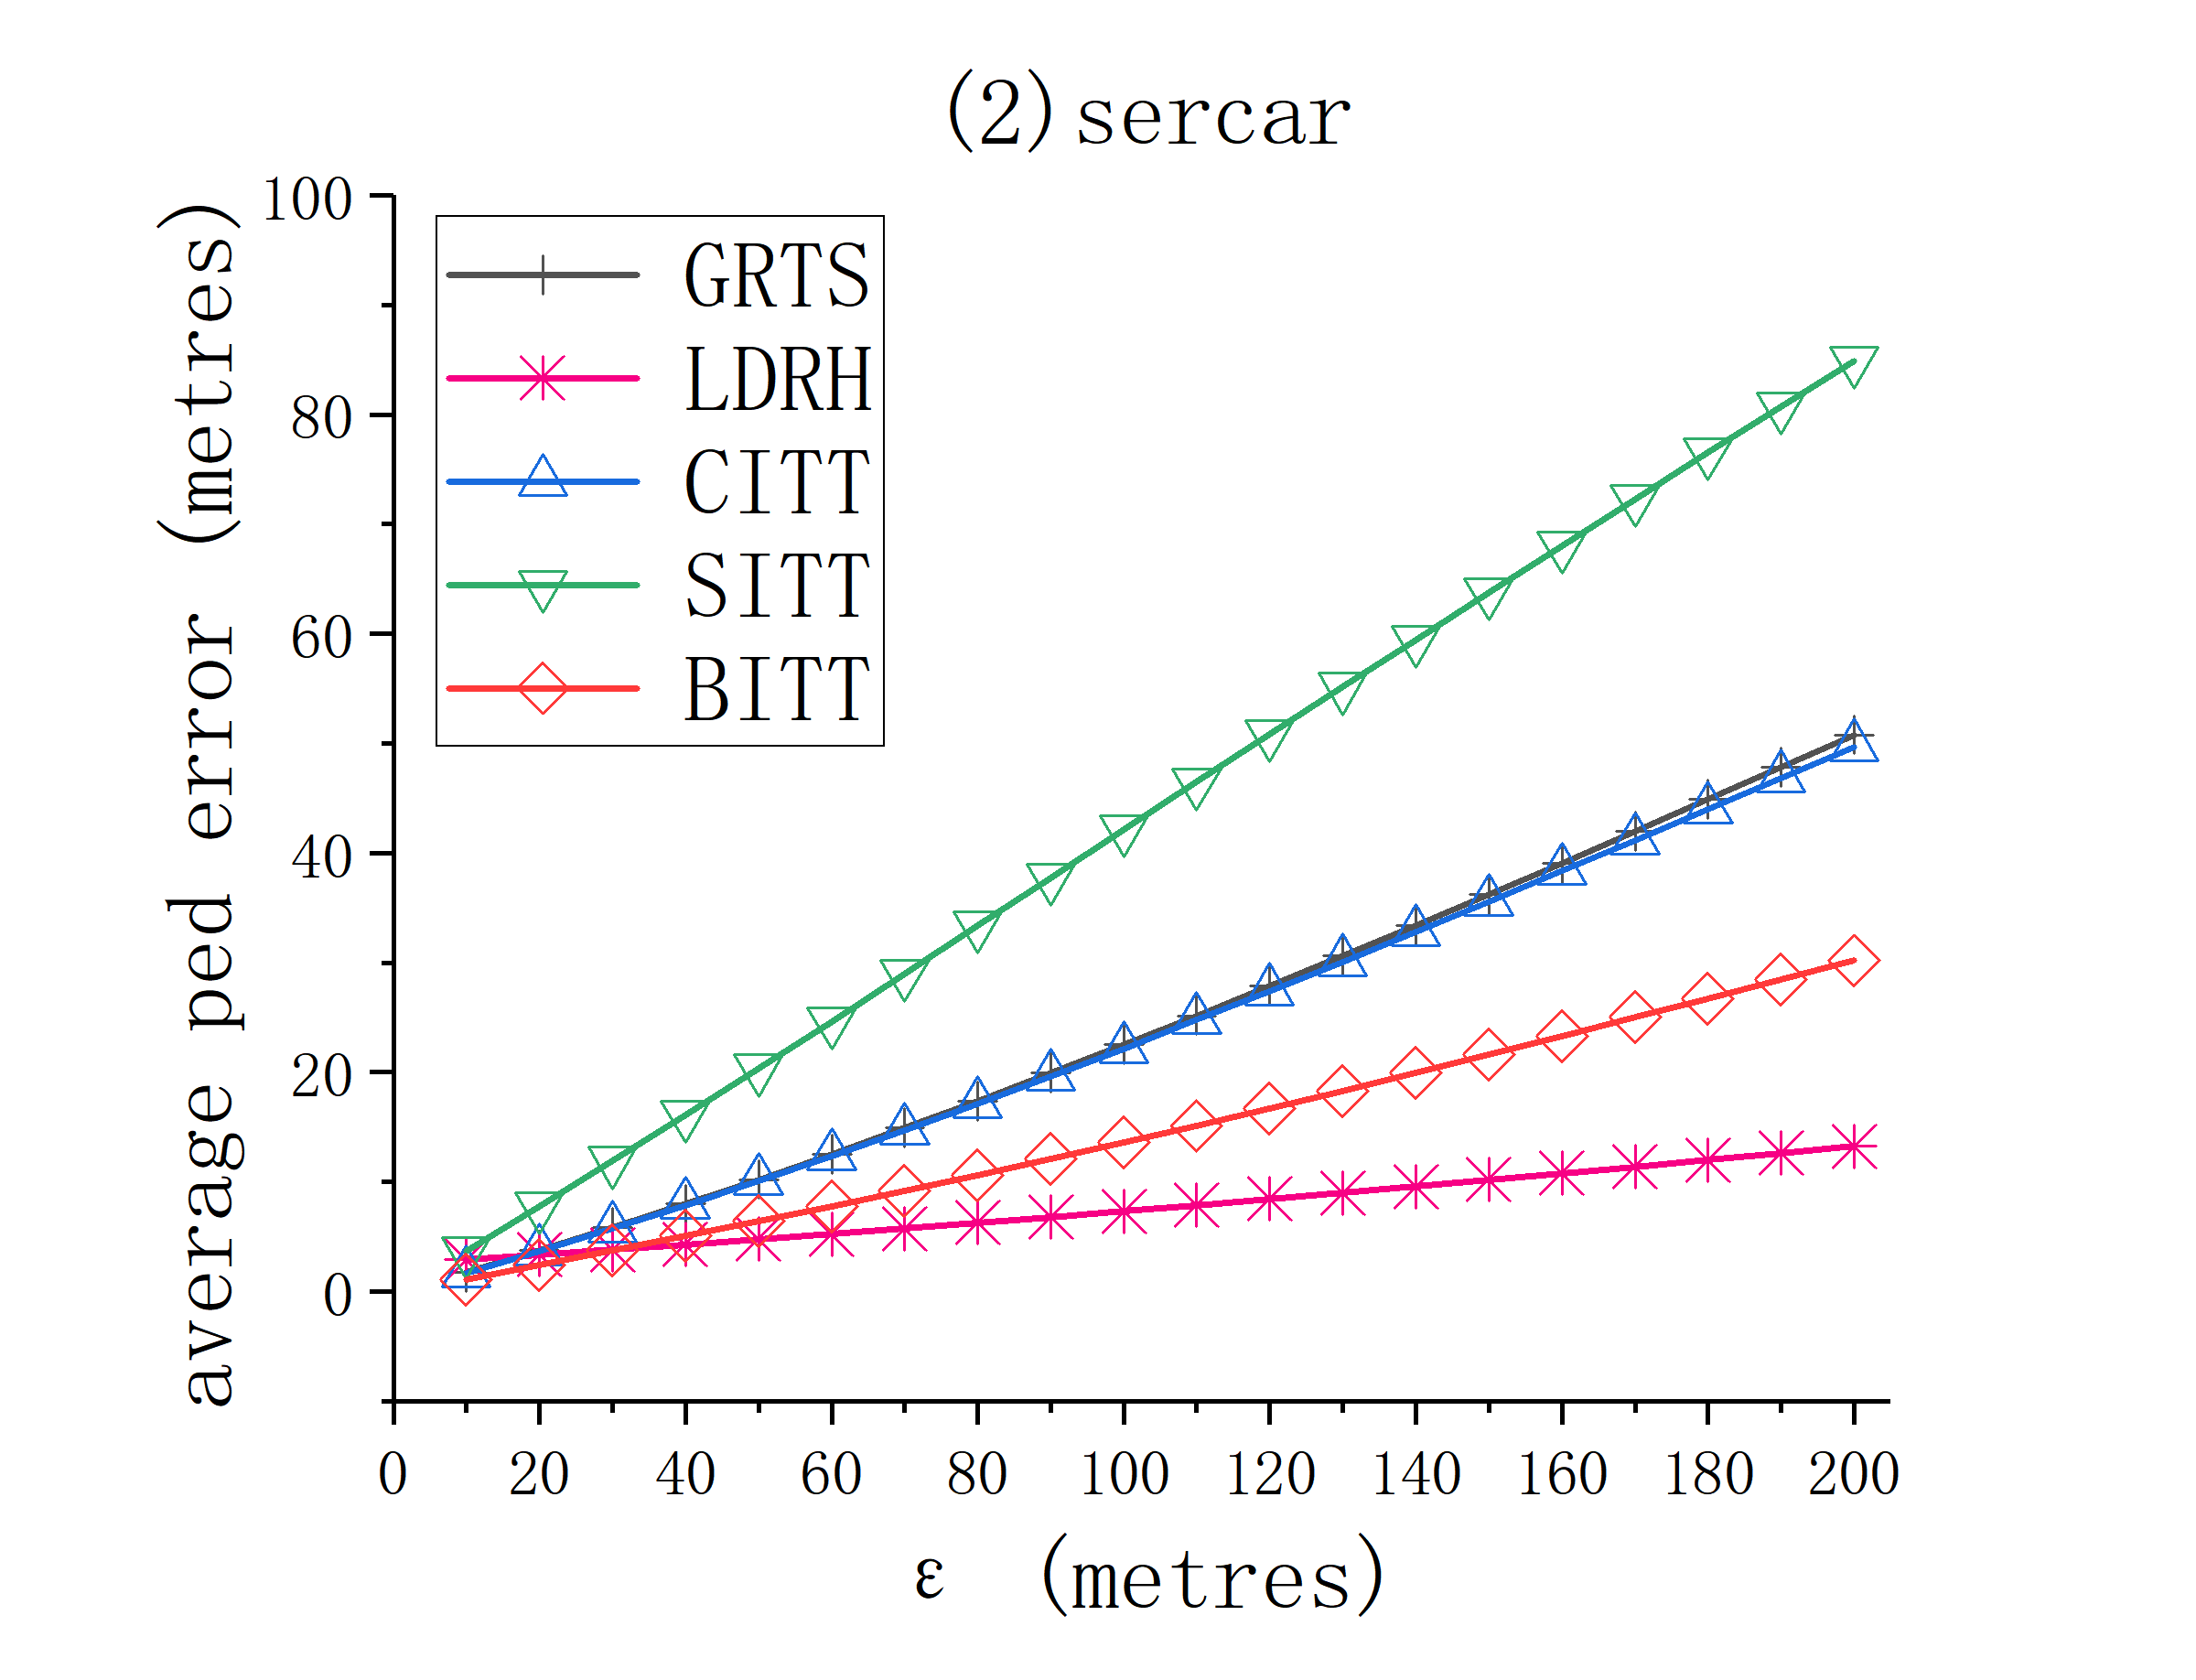
\includegraphics[scale = 0.210]{figures/Fig-sercar-ped-error.png}\hspace{1ex}
	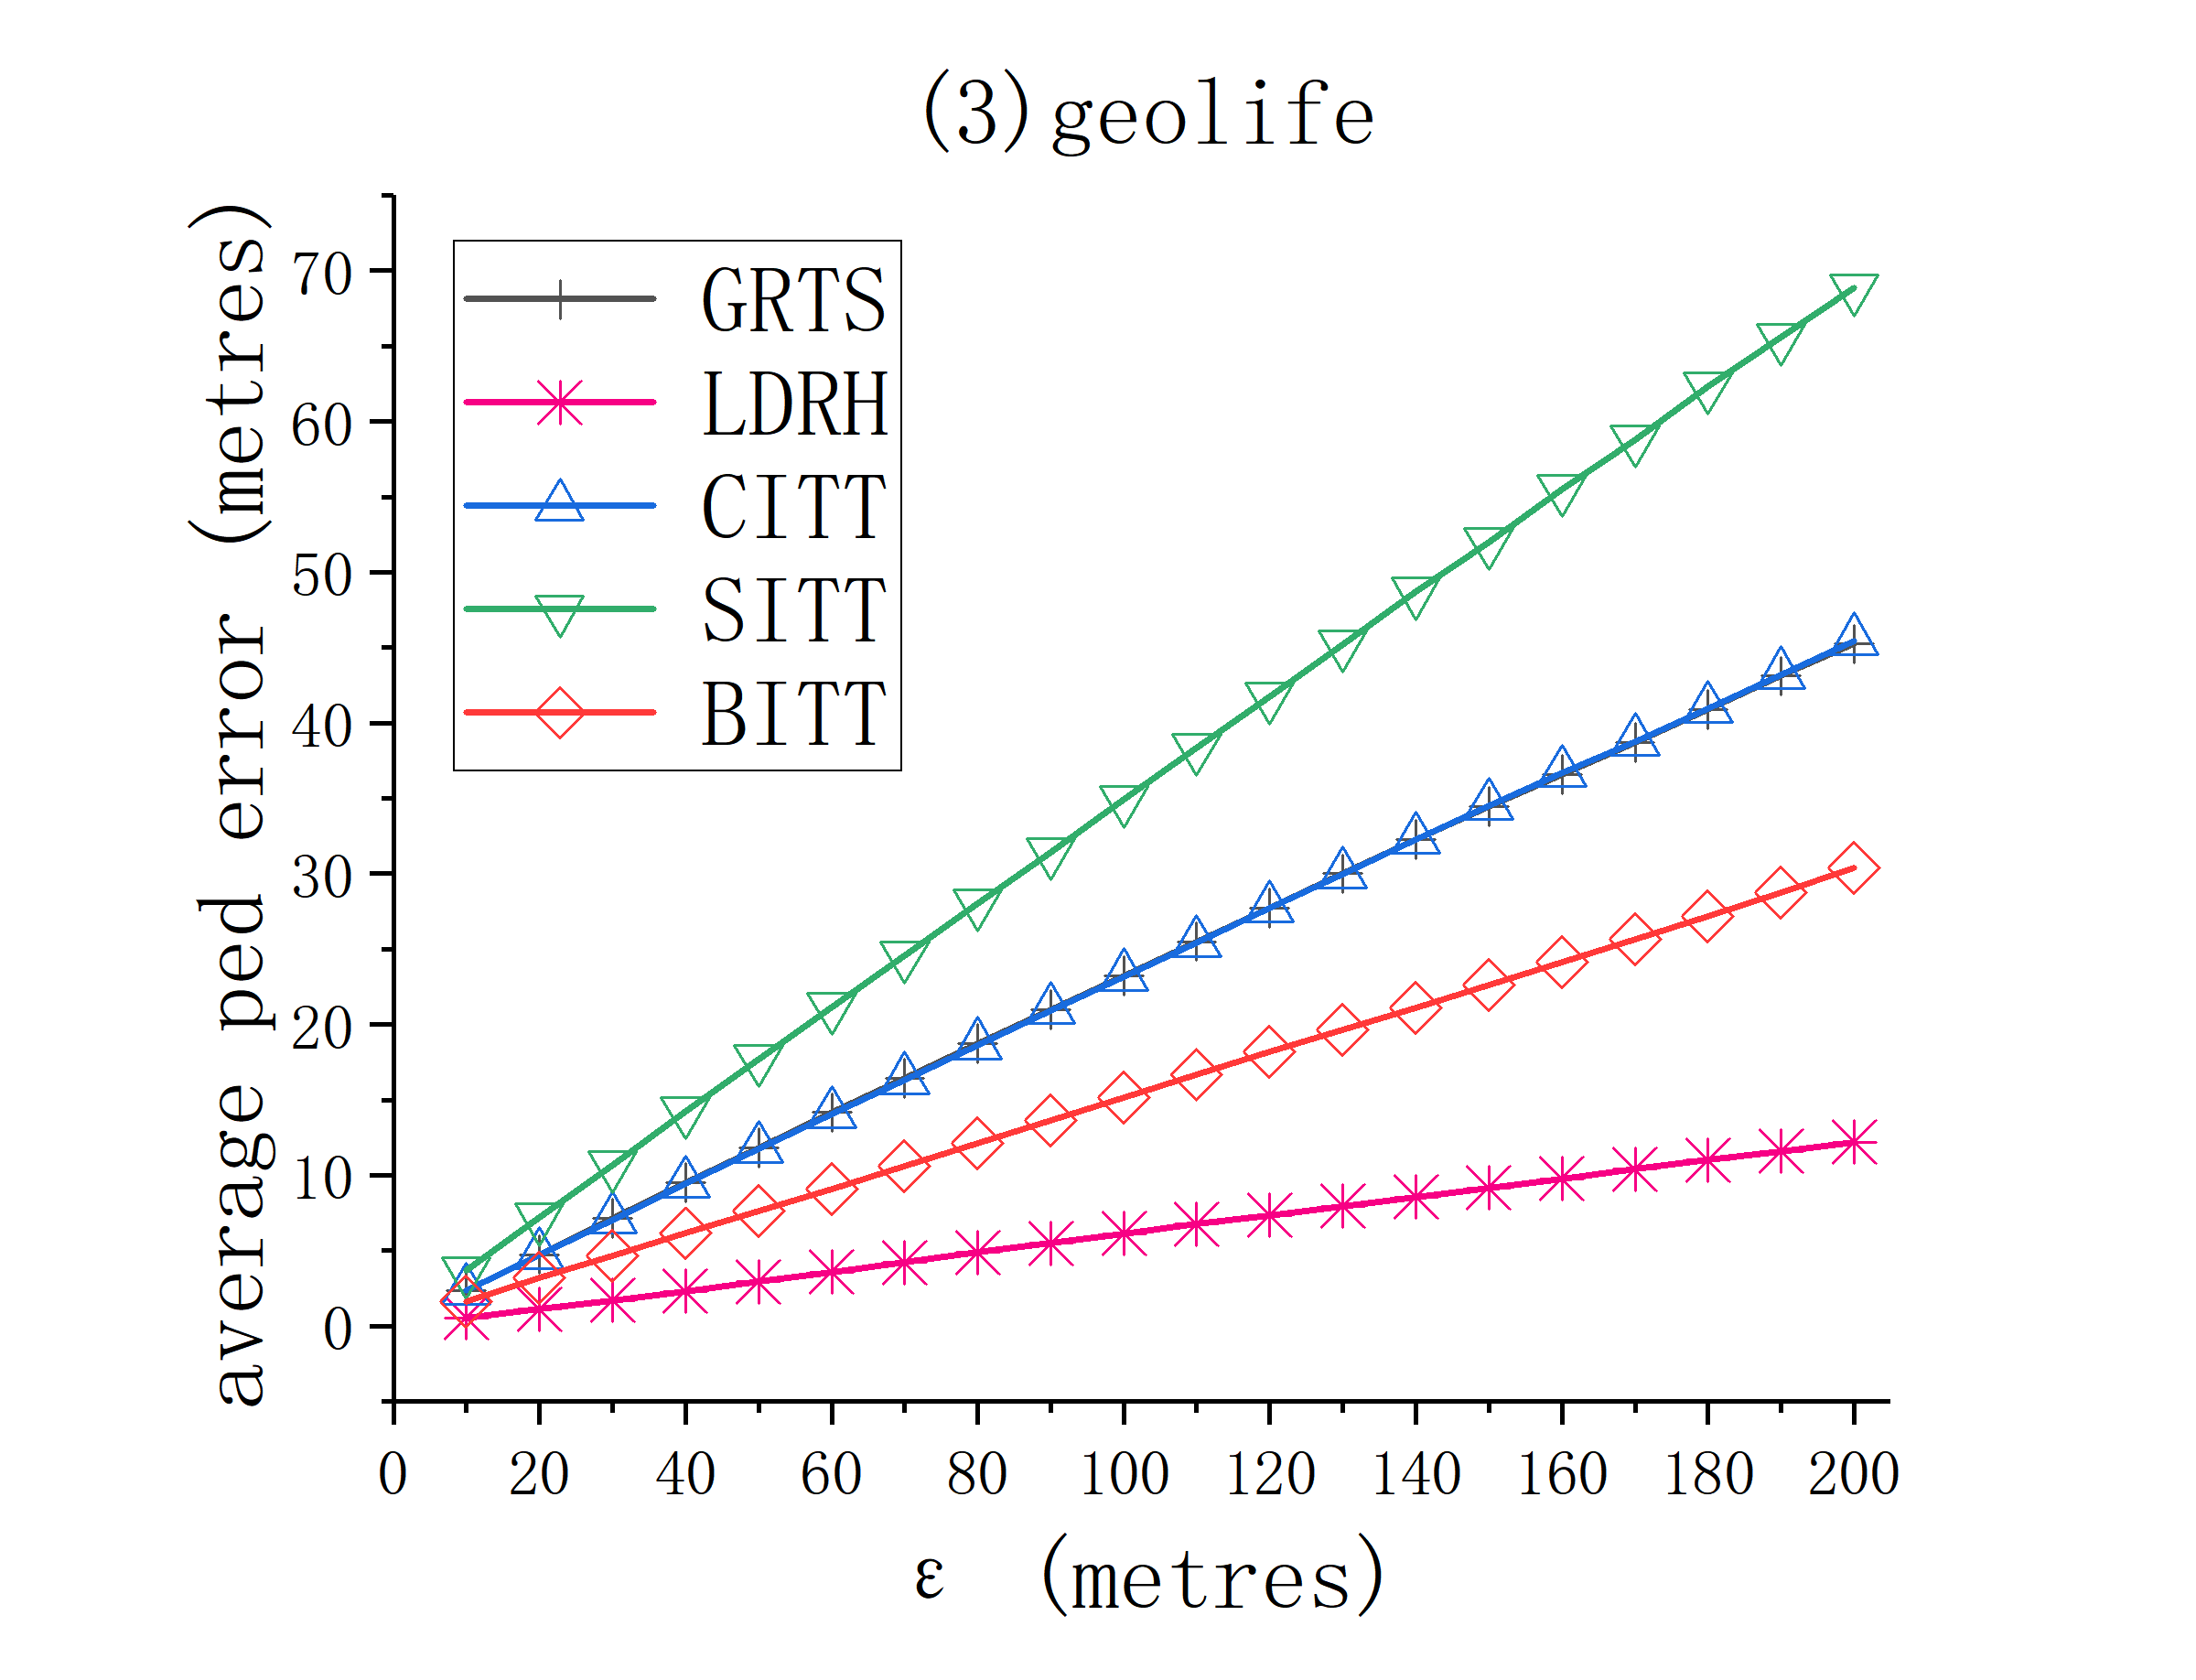
\includegraphics[scale = 0.210]{figures/Fig-geolife-ped-error.png}\hspace{1ex}
	%\vspace{-1ex}
	\caption{\small Evaluation of ped error: varying error bounds $\epsilon_{sed}$ and $\epsilon_{ped}$.}
	\label{fig:ped-error}
	%\vspace{-1ex}
\end{figure*}

\stitle{Average errors.}
%The results are reported in Figures~\ref{fig:sed-error} and Figure~\ref{fig:ped-error}.
\ni (1) Average errors increase with the increase of $\epsilon_{sed}$ and $\epsilon_{ped}$.

\ni (2) The average sed errors of these algorithms from the largest to the smallest are \sitt, \grts (\citt) and \ldrh. Among them, the average sed errors of \citt is very close to \grts.
The average sed errors of algorithms \citt and \sitt are on average
($412.7\%$, $222.8\%$, $350.1\%$)
and ($842.0\%$, $857.5\%$, $1452.5\%$)
of \ldrh and ($103.1\%$, $98.4\%$, $100.5\%$) and
($209.9\%$, $442.9\%$, $414.0\%$)
of \grts on datasets (\mopsi, \sercar, \geolife), respectively.

\ni (3) The average ped errors of these algorithms from the largest to the smallest are \sitt, \grts (\citt) and \ldrh. Among them, the average ped errors of \citt is very close to \grts.
The average ped errors of algorithms \citt and \sitt are on average
($452.2\%$, $278.1\%$, $388.9\%$)
and ($550.5\%$, $517.0\%$, $589.0\%$)
of \ldrh and ($102.0\%$, $98.3\%$, $99.7\%$) and
($123.9\%$, $187.0\%$, $150.9\%$)
of \grts on datasets (\mopsi, \sercar, \geolife), respectively.

\ni (4) The average sed errors and the average ped errors of algorithm \bitt are between \citt and \sitt.



\begin{figure*}[tb!]
	\centering
	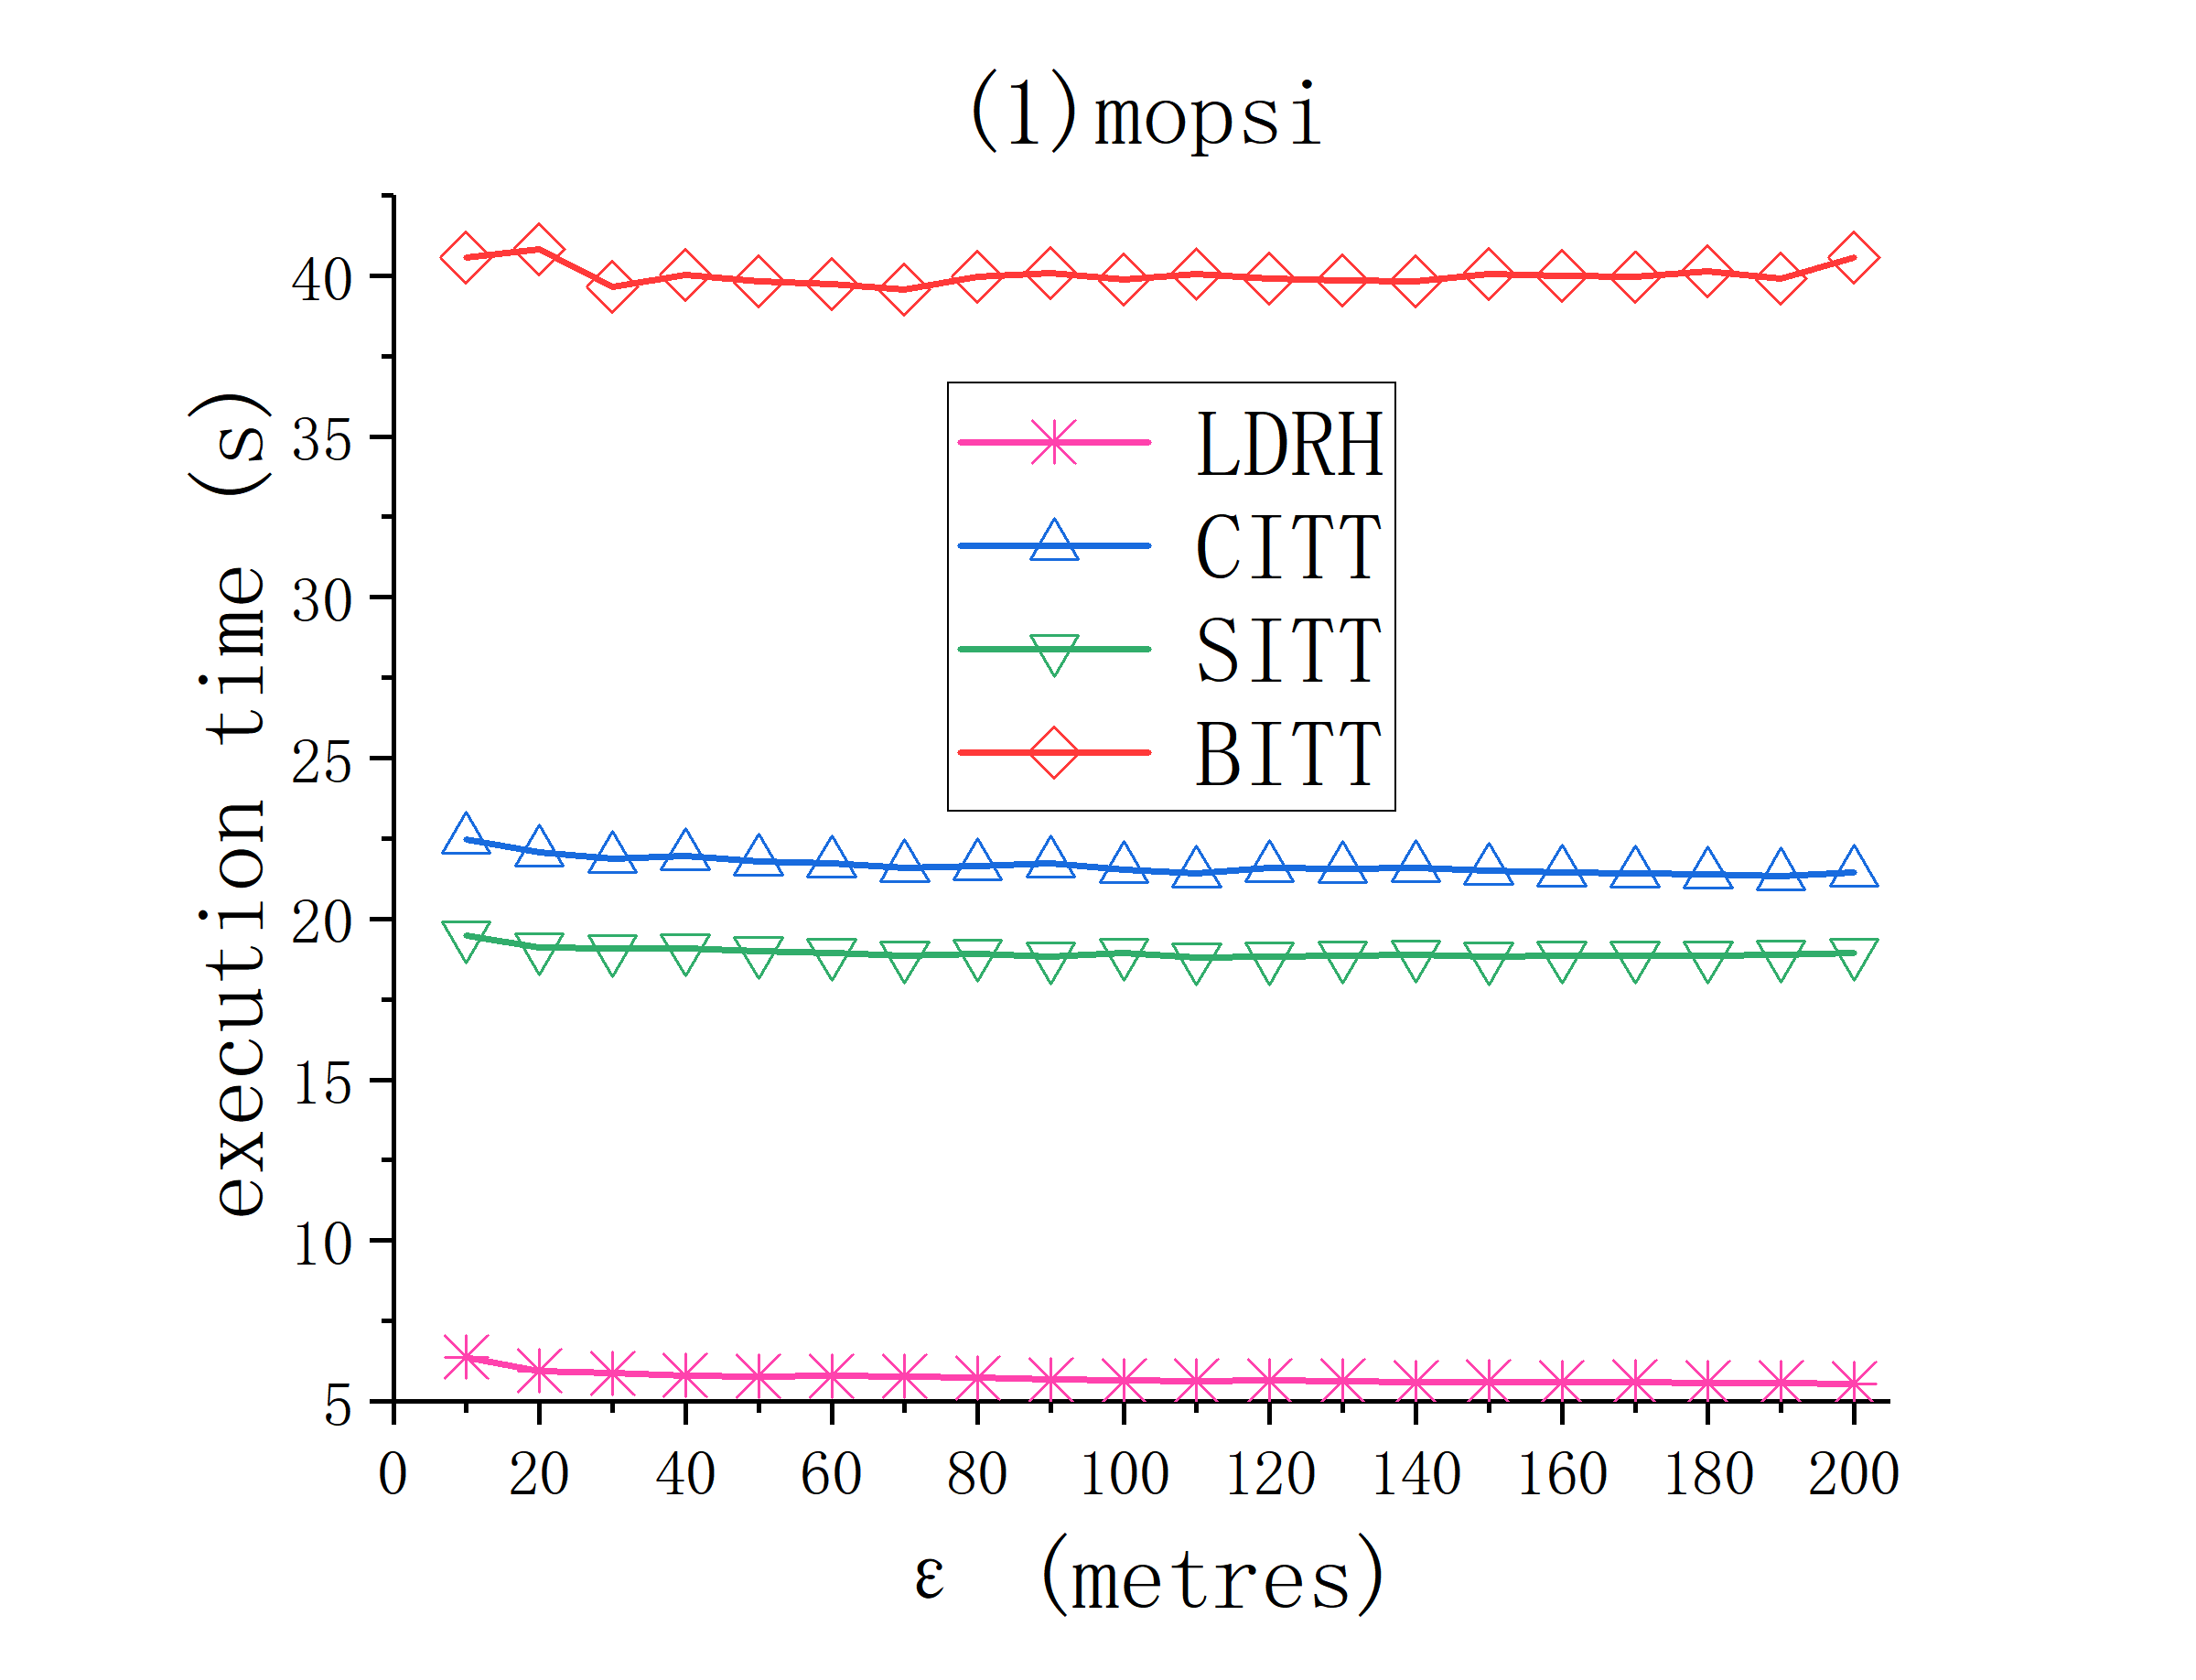
\includegraphics[scale = 0.210]{figures/Fig-mopsi-running-time.png}\hspace{1ex}
	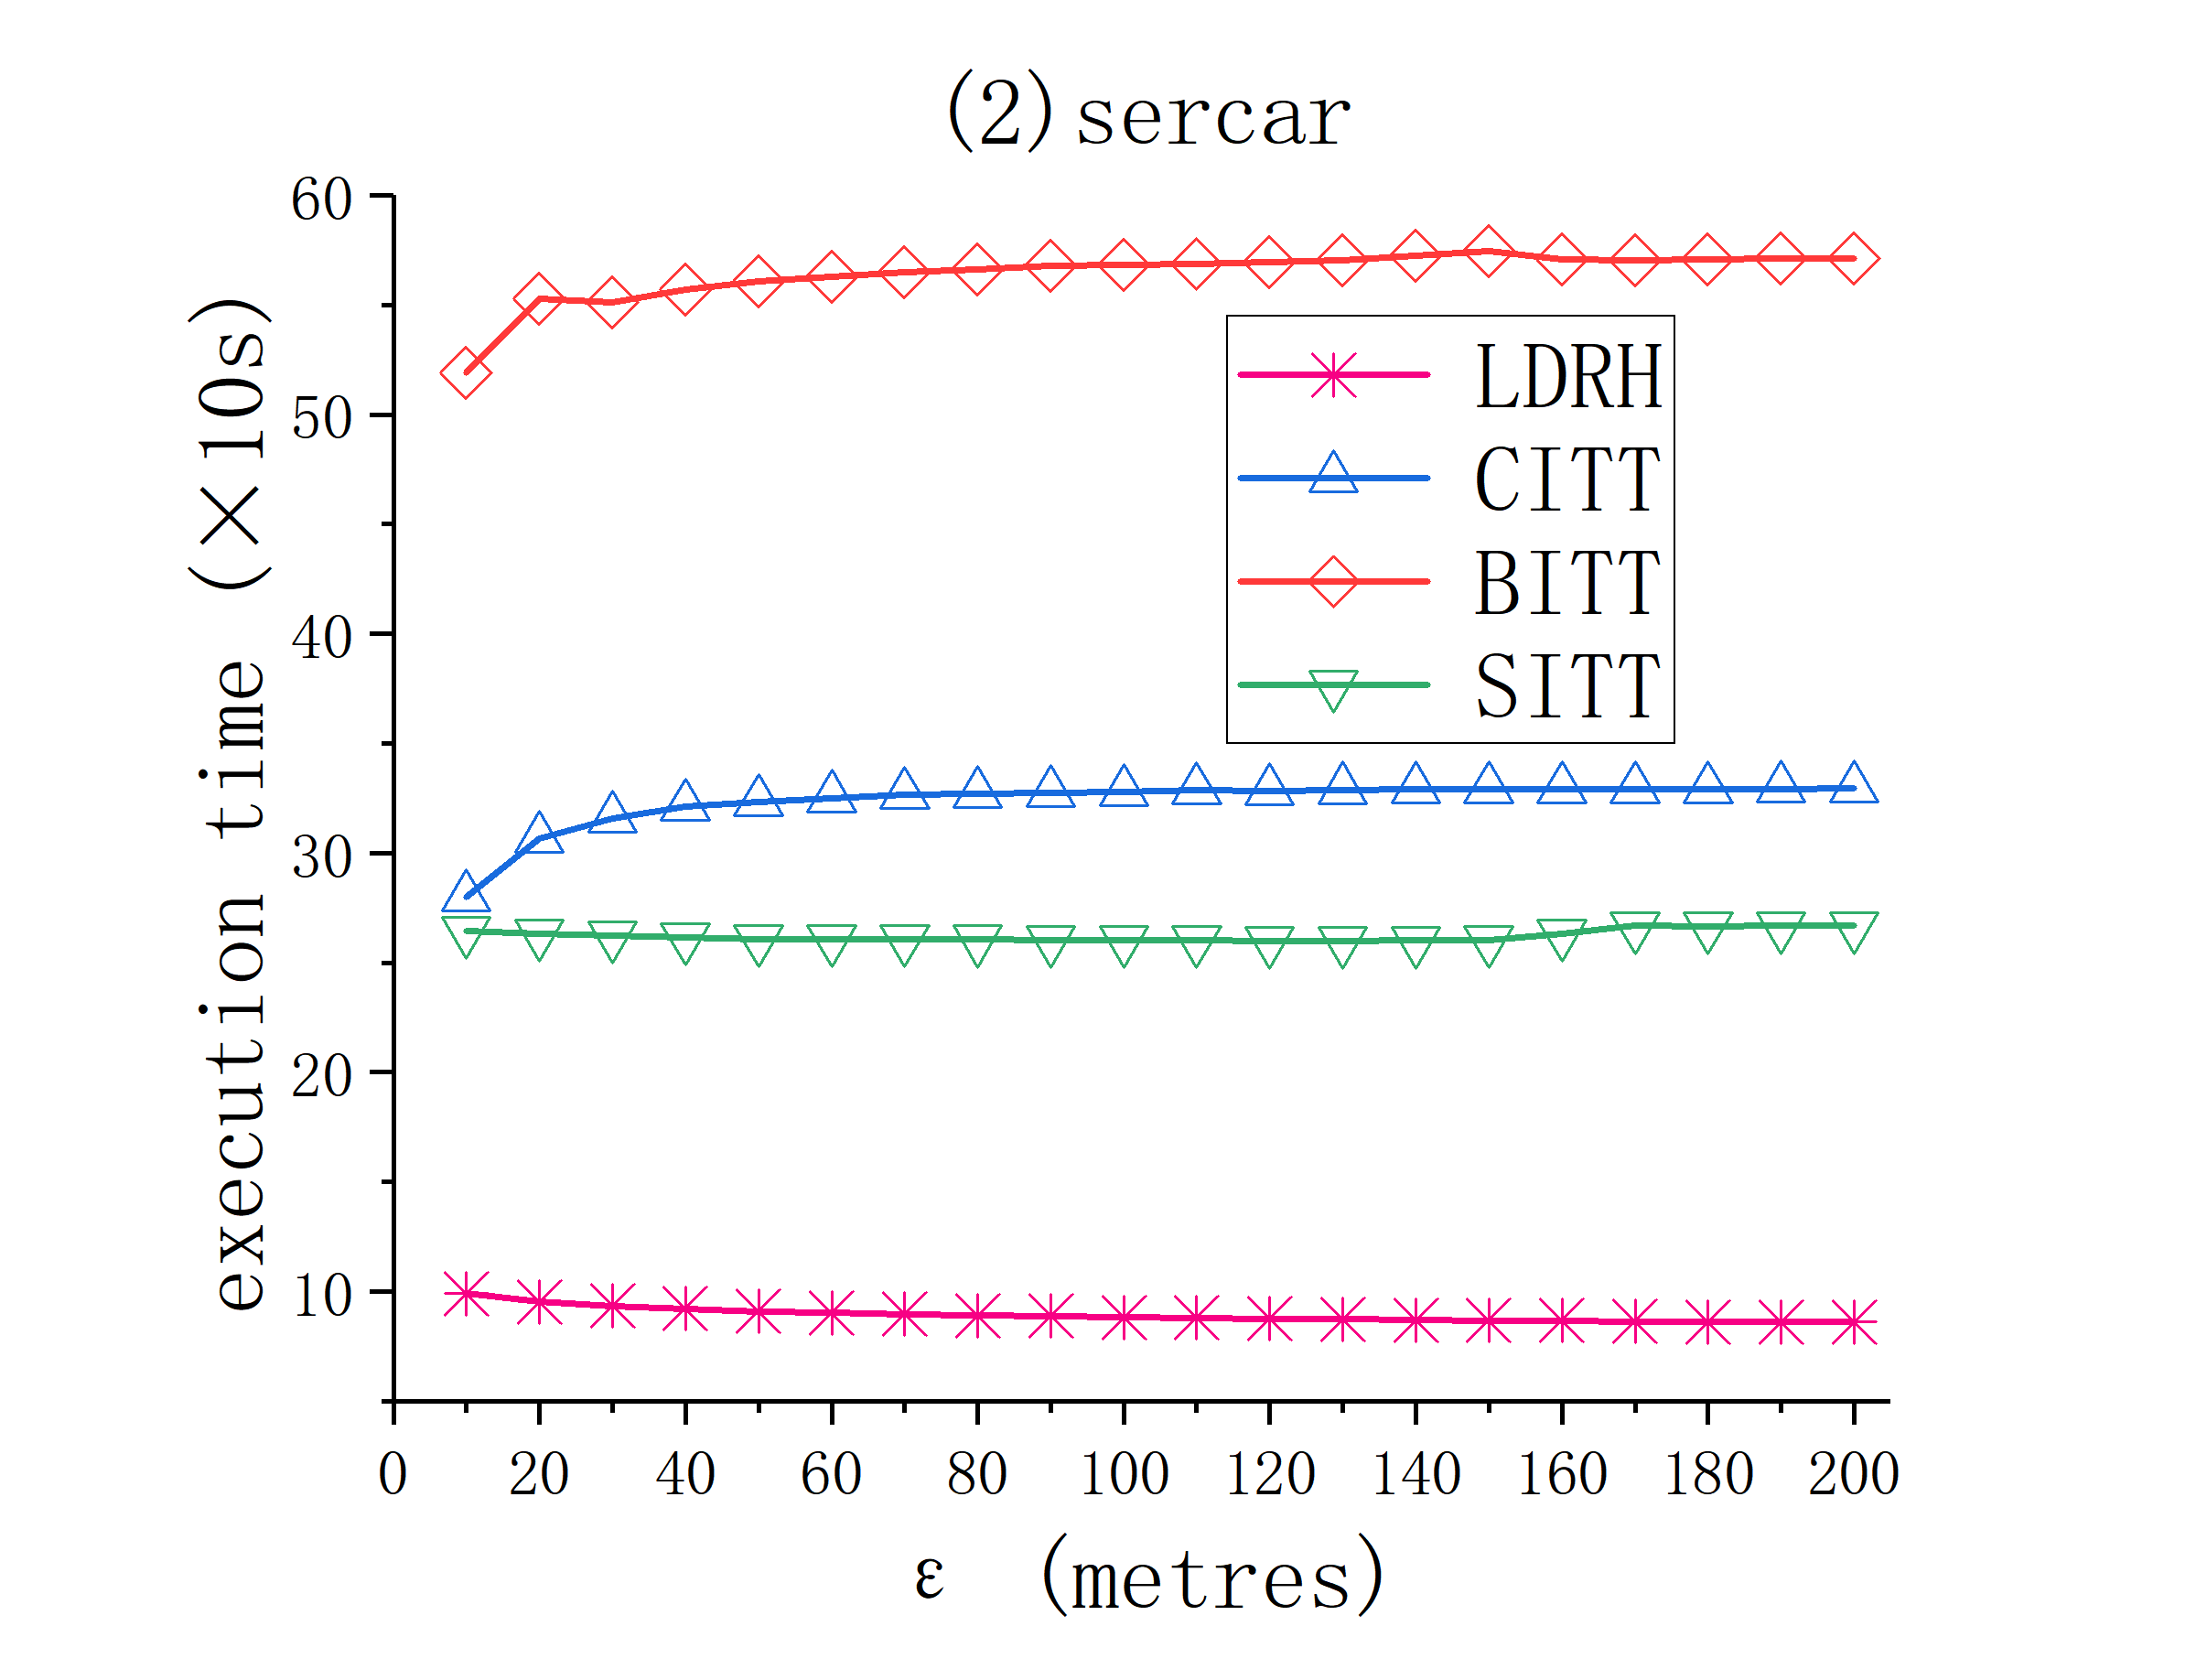
\includegraphics[scale = 0.210]{figures/Fig-sercar-running-time.png}\hspace{1ex}
	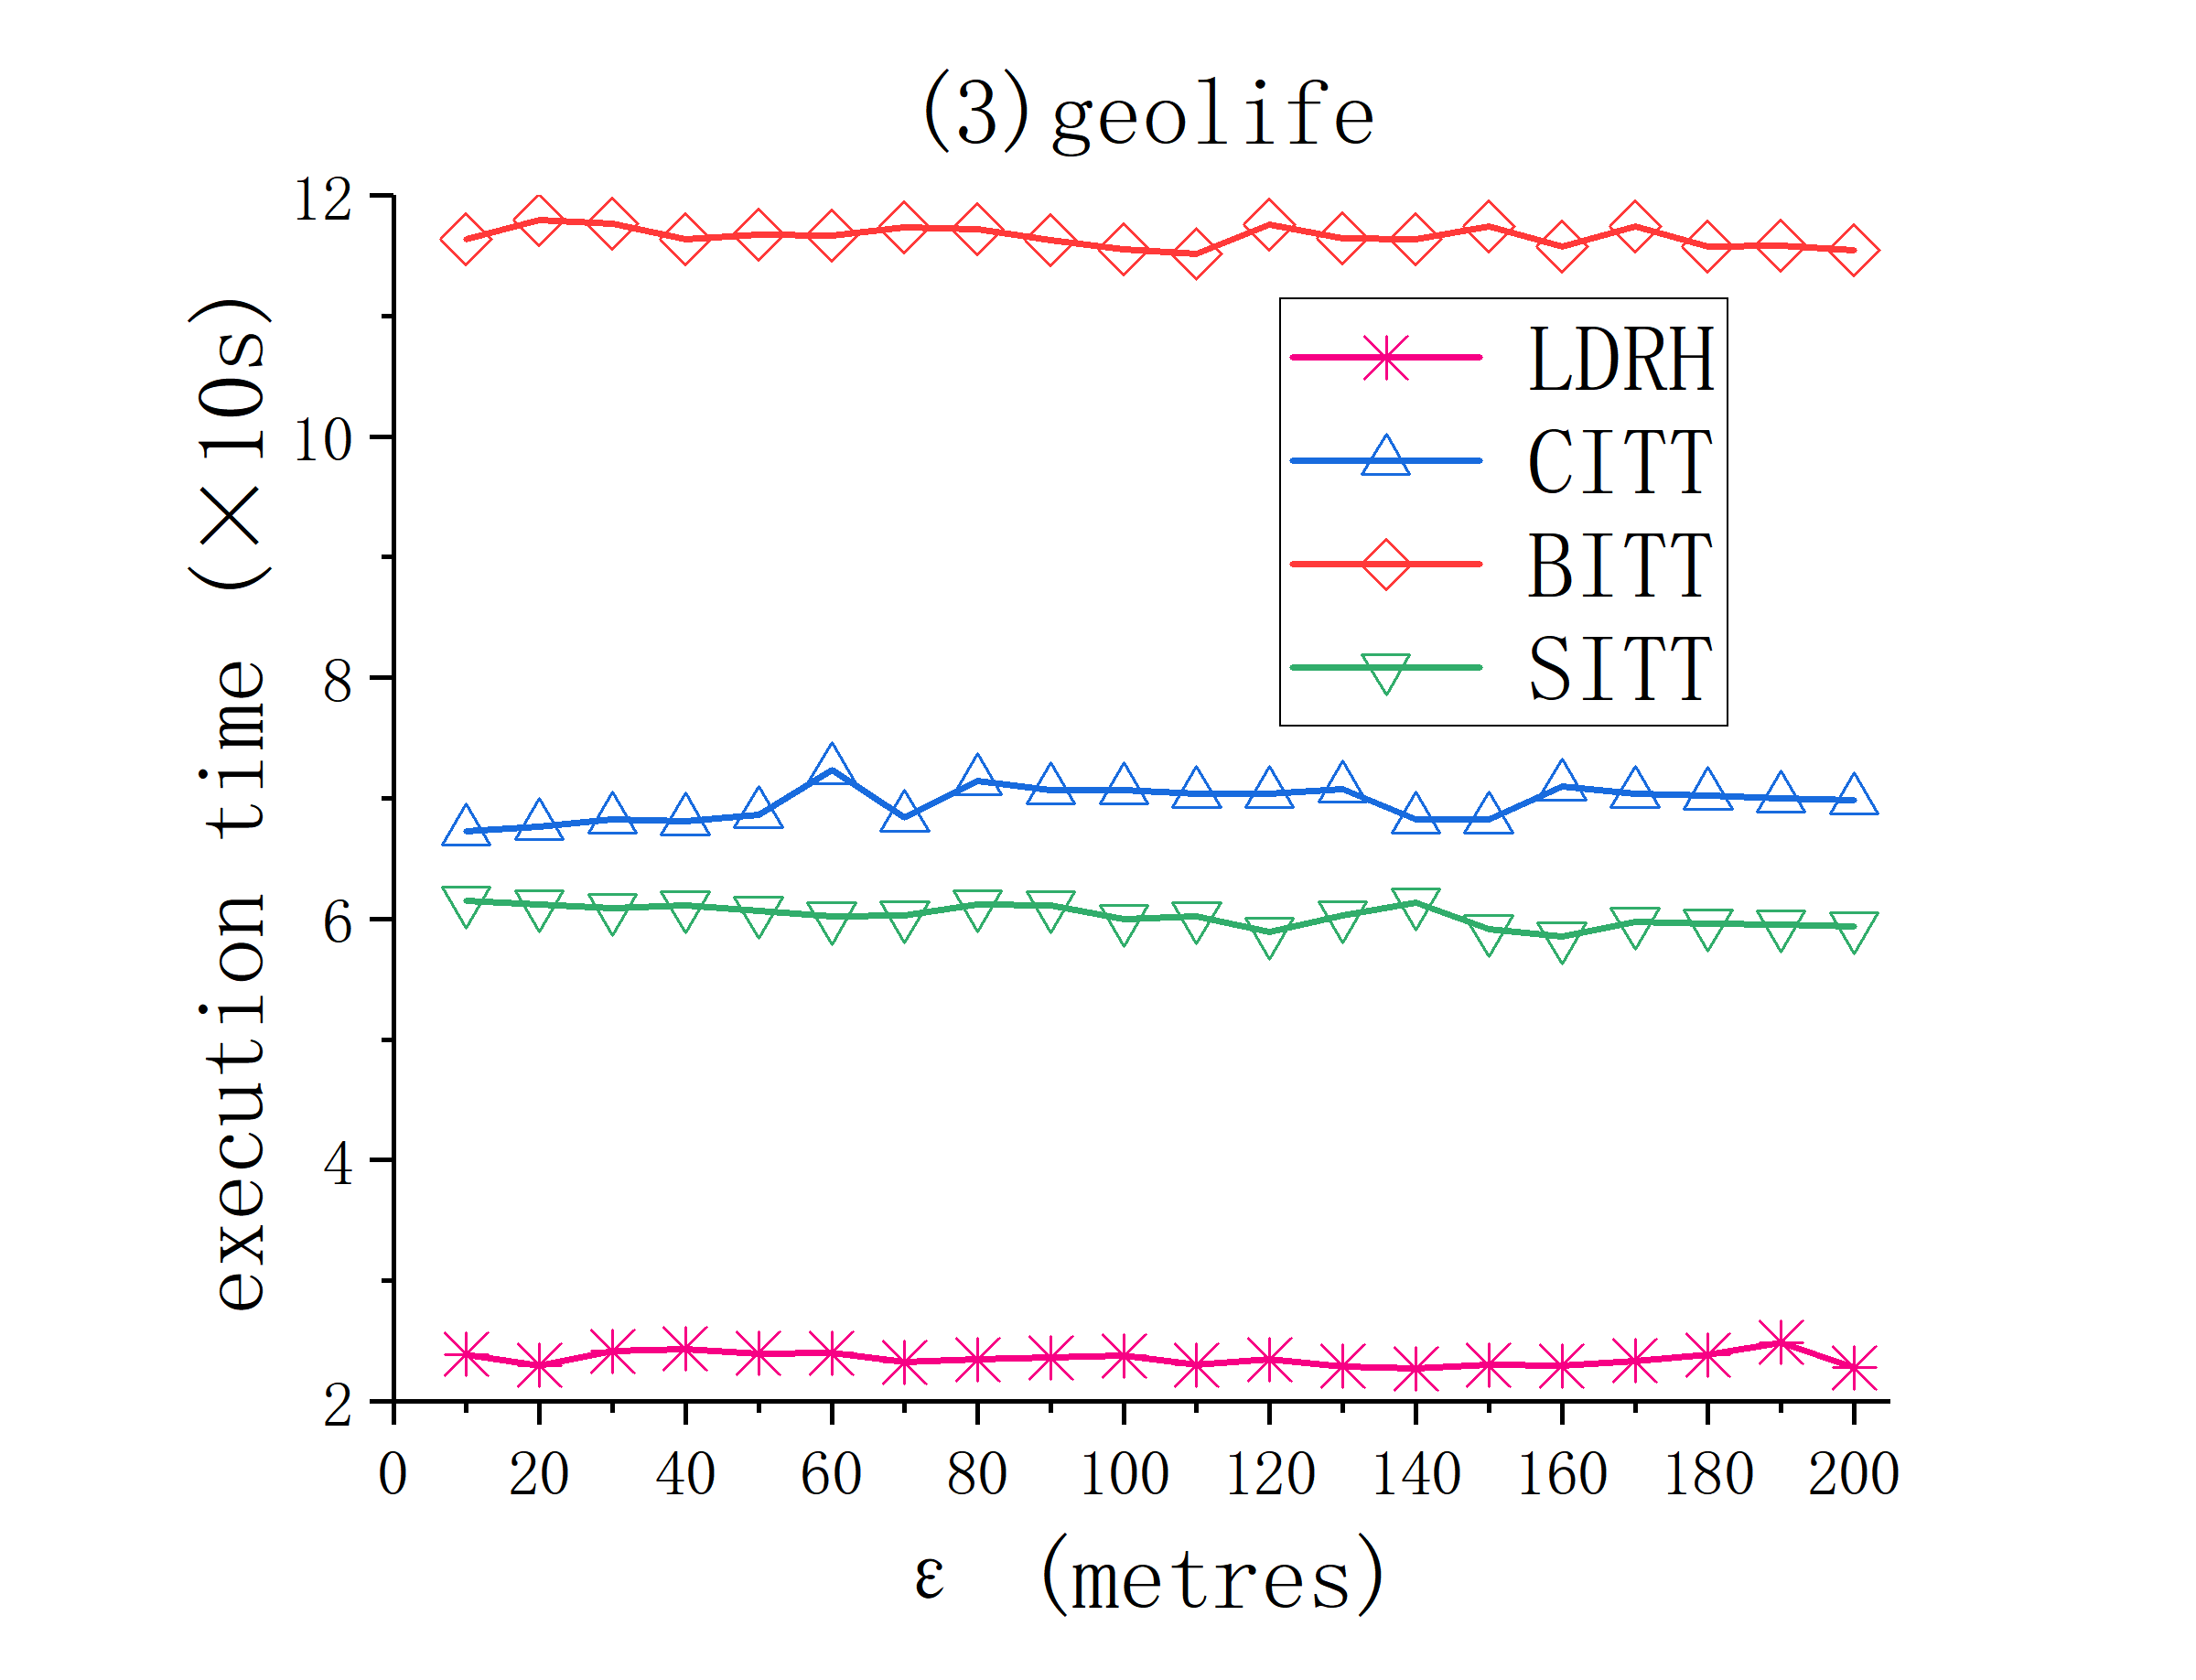
\includegraphics[scale = 0.210]{figures/Fig-geolife-running-time.png}\hspace{1ex}
	%\vspace{-1ex}
	\caption{\small Evaluation of running time: varying error bounds $\epsilon_{sed}$ and $\epsilon_{ped}$.}
	\label{fig:running-time}
	%\vspace{-1ex}
\end{figure*}

\stitle{Running time.}
%%%%%%%%%%%%%%%%% running time
%In this part of experiments, we compare the running time of our algorithms \citt, \sitt and \bitt with \ldrh and \grts.
%The results are reported in Figure~\ref{fig:running-time}. 
Since the running time of \grts is thousands of times slower than other algorithms, it is not shown in Figure~\ref{fig:running-time}.

\ni (1) The running times of these algorithms from the largest to the smallest are \grts, \bitt, \citt, \sitt and \ldrh, on all datasets.
The average running times of algorithms \citt and \sitt are on average
($378.8\%$, $363.2\%$, $296.4\%$)
and ($331.5\%$, $294.1\%$, $256.4\%$)
of \ldrh and ($0.607\%$, $21.7\%$, $0.704\%$) and
($0.529\%$, $18.1\%$, $0.623\%$)
of \grts on datasets (\mopsi, \sercar, \geolife), respectively.

\ni (2) The running time of \bitt is approximately the sum of \citt and \sitt. Because it contains the judgment conditions in \citt and \sitt.
